\newpage

\section*{Anhang}
  \addcontentsline{toc}
    {section}
    {Anhang}



\subsection*{Elektronischer Anhang}\label{elect-anhang}
\addcontentsline{toc}
{subsection}
{Elektronischer Anhang}

Diese Dokumentation wurde zusammen mit einem elektronischen Anhang in Form einer ZIP-Datei abgegeben. Darin befinden sich der Simulator Programmiercode inklusive dessen Ergebnisse und die erstellten CAD Dateien.

TODO LIST OF WHATS IN THERE

\newpage
\subfile{parts/x-projektplanung}
\newpage

%%%%%%%%%%%%%%%%%% Aufgabenstellung

\subsection*{Originale Aufgabenstellung}\label{aufgabenstellung}
\addcontentsline{toc}
{subsection}
{Originale Aufgabenstellung}

Nachfolgend ist die originale Aufgabenstellung angehängt.

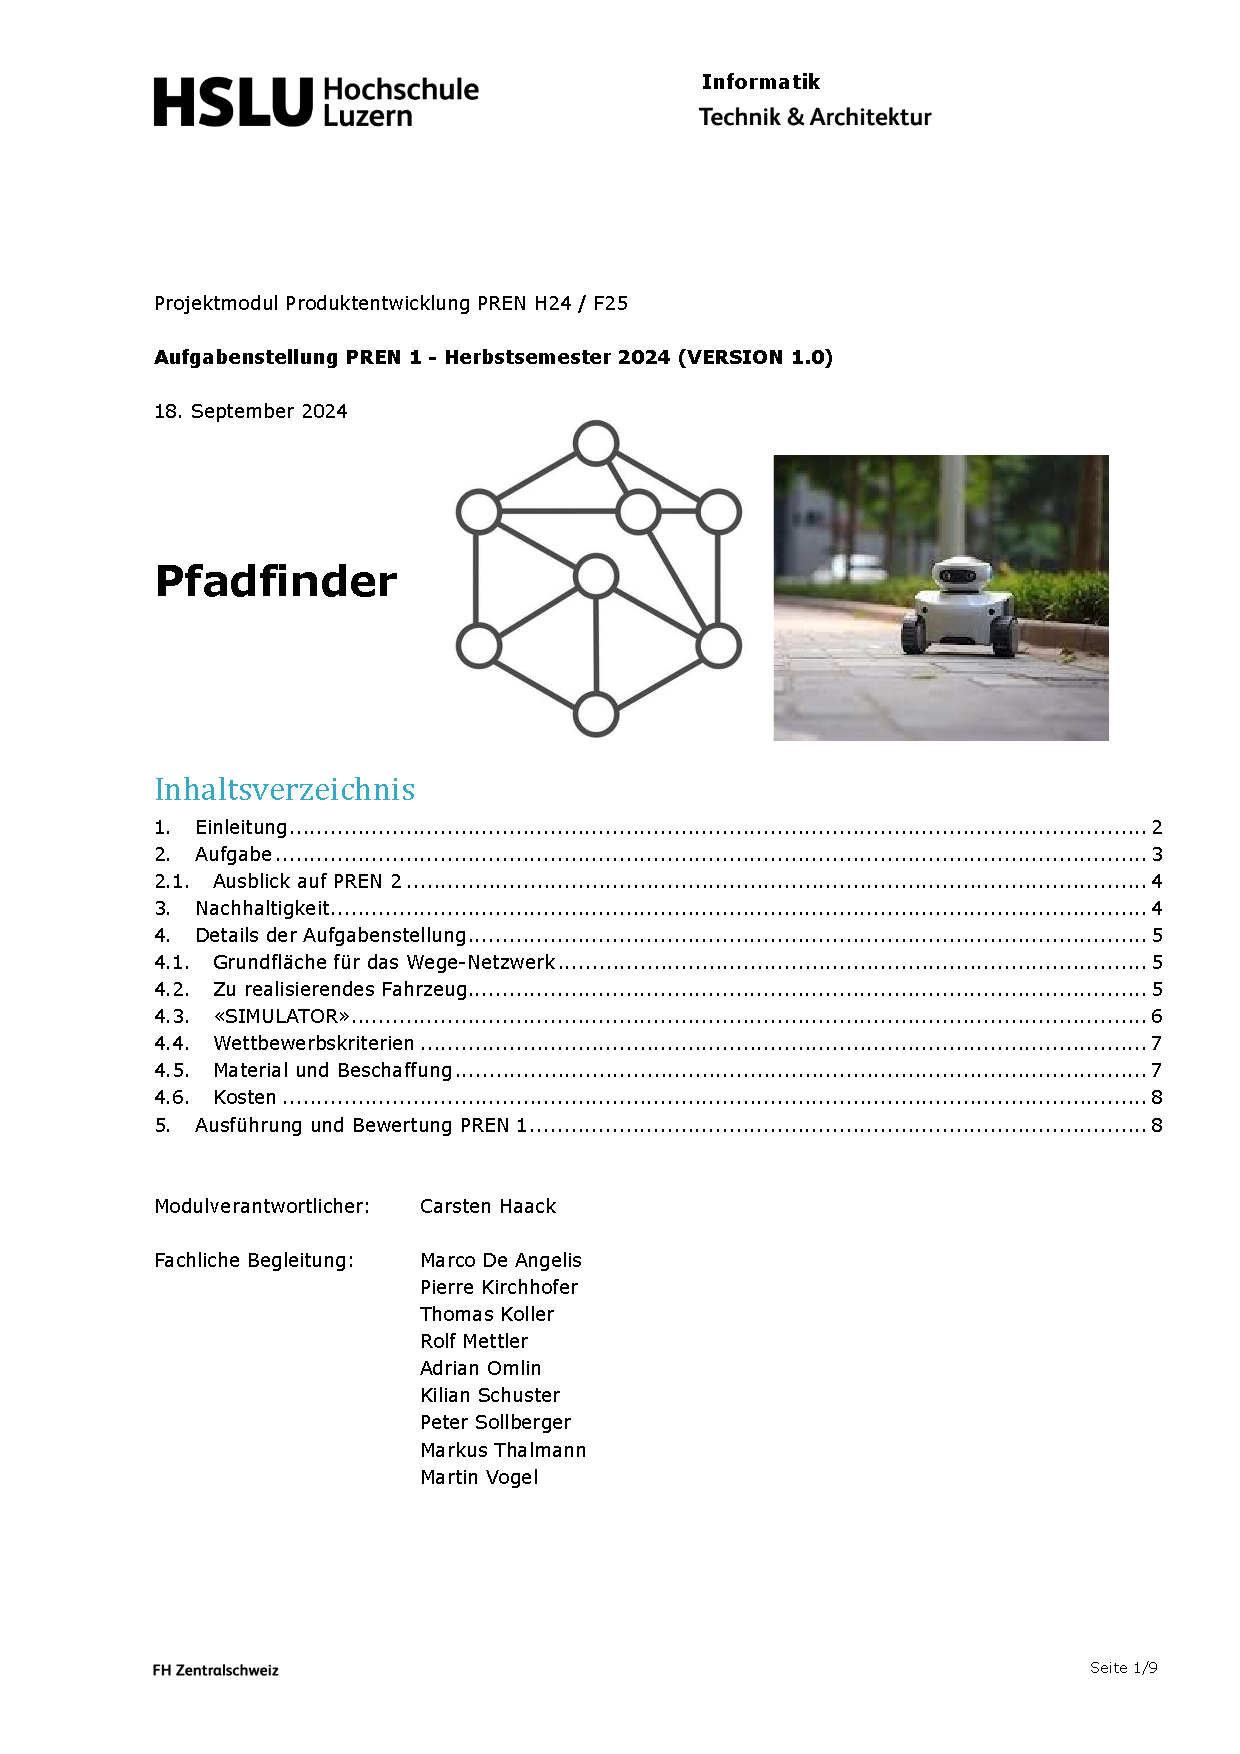
\includepdf[pages=-]{assets/projektmanagement/AufgabenstellungPREN1HS24.pdf}

%%%%%%%%%%%%%%% Anforderungsliste %%%%%%%%%%%%%%%%%%%%%%%%%

\subsection*{Anforderungsliste}\label{anforderungliste}
  \addcontentsline{toc}
    {subsection}
    {Anforderungsliste}
Die  Anforderungsliste ist ersichtlich in Tabellen \ref{table:anforderungsliste_page1} und \ref{table:anforderungsliste_page2}.

\begin{table}[H]
\centering
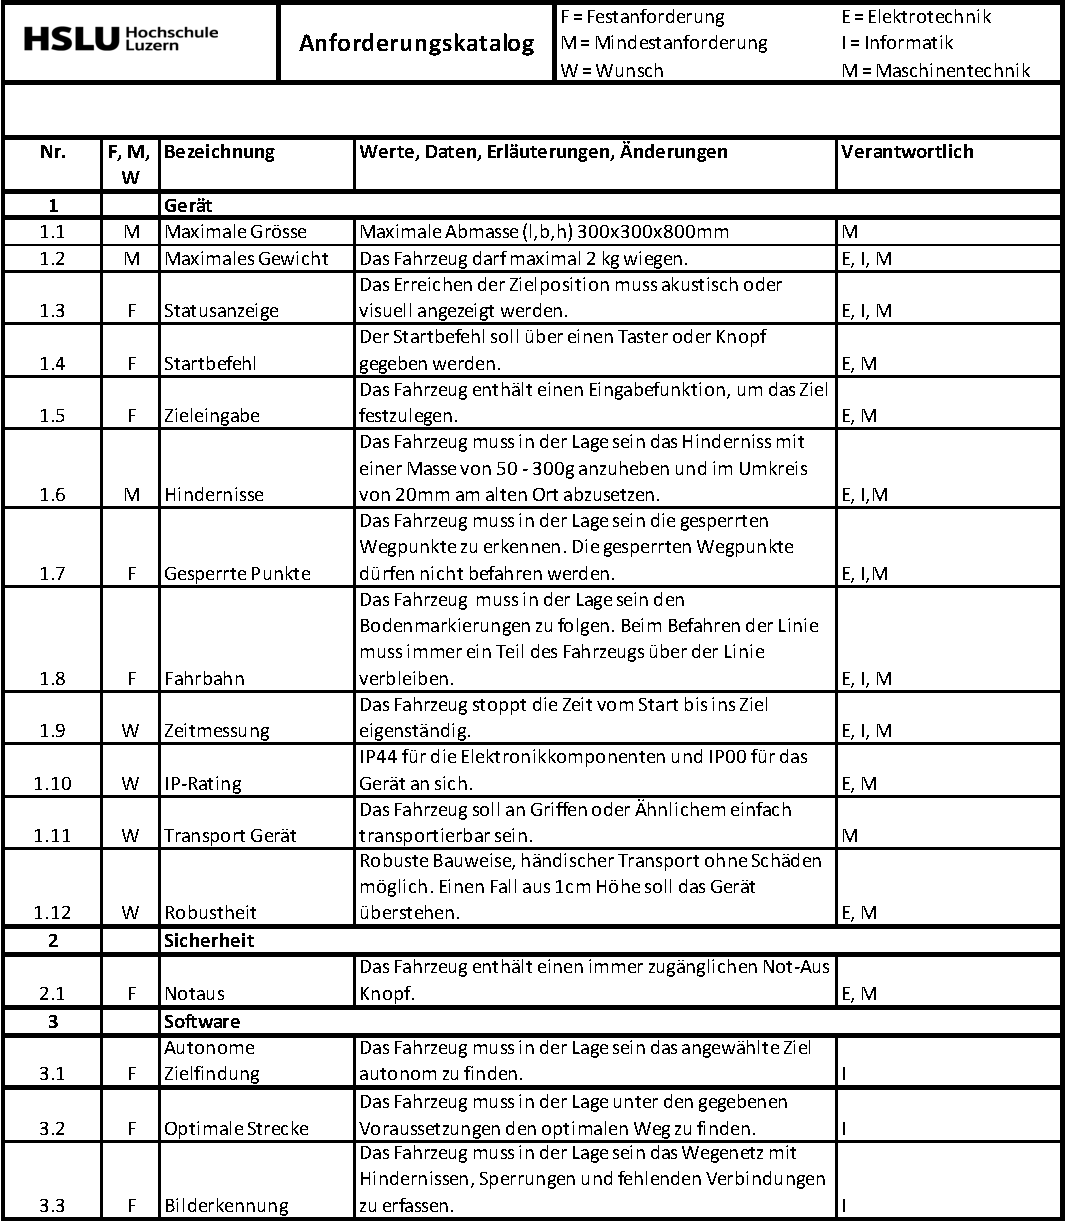
\includegraphics[width=\textwidth]{assets/projektmanagement/Anforderungsliste_V1.01_page1.pdf}
\caption{Anforderungsliste Teil 1}
\label{table:anforderungsliste_page1}
\end{table}
\newpage

\begin{table}[H]
\centering
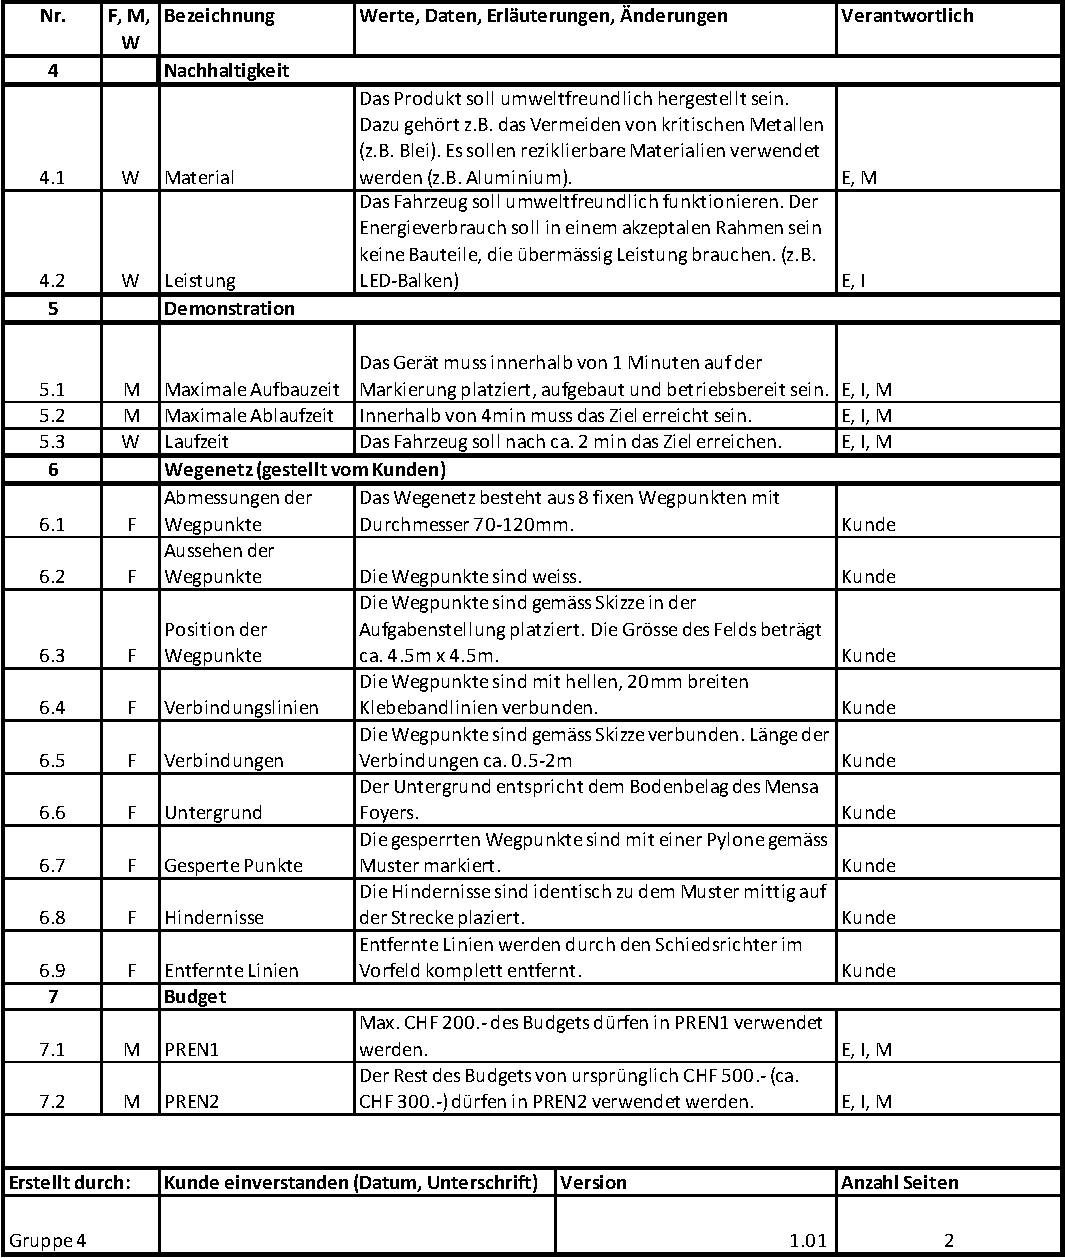
\includegraphics[width=\textwidth]{assets/projektmanagement/Anforderungsliste_V1.01_page2.pdf}
\caption{Anforderungsliste Teil 2}
\label{table:anforderungsliste_page2}
\end{table}
\newpage


%%%%%%%%%%%%%%%% Model Evaluation %%%%%%%%%%%%%%%%%%%%%%%%%5

\subsection*{YOLOv11 Model Evaluation}\label{model-evaluation}
  \addcontentsline{toc}
    {subsection}
    {YOLOv11 Model Evaluation}

Damit Pylonen, Barrieren und Knoten erkannt werden können, wird ein Model trainiert. Insgesamt wurden über 30 verschiedene YOLO Models trainiert. Viele davon wurden bereits in einem vorherigen Schritt aussortiert, da einige sehr offensichtlich schlechte Performance aufwiesen aufgrund davon, wie es die Objekte erkannt, beziehungsweise nicht erkannt hat. Auf der folgenden Seite ist eine Tabelle angehängt, in der die relevanten Models miteinander verglichen werden und das beste Model gewählt wurde.

Die Model Performance wird an folgenden Parametern gemessen:\cite{model-performance}

\begin{itemize}
    \item Confusion Matrix: Zeigt was das Model vorhergesagt hat und was tatsächlich zu sehen war. Je 'diagonaler' die Matrix, desto besser.
    \item F1-Confidence: Zeigt die Balance zwischen Confidence (Wahrscheinlichkeit, dass Vorrausgesagtes stimmt) und F1 Score (Harmonischer Durchschnitt von Recall und Precision). Je höher der F1 Wert, desto besser.
    \item Precision-Confidence: Zeigt die Balance zwischen Precision (Anteil von 'True Positives'; wenn Model sagt, es gibt einen Knoten, wie akkurat ist diese Deutung?) und Confidence. Je tiefer die Confidence, desto besser, da dadurch der hoechste Praezisionswert bereits bei einer tieferen Confidence erreicht wird.
    \item Precision-Recall: Zeigt die Balance zwischen Precision und Recall (Faehigkeit, alle Instanzen zu erkennen). Je hoeher die Precision, desto besser.
    \item Recall-Confidence: Zeigt die Balance zwischen Recall und Confidence. Je höher der Recall, desto besser.
    \item Lernverlauf: Zeigt inwiefern der Verlust (Unterschied zwischen Vorhergesagtem und Realität) sinkt bei den Trainingsdaten und den Validationsdaten. Beginnt der Verlust bei der Validation zu steigen, deutet dies auf Overfitting hin\footnote{https://developers.google.com/machine-learning/crash-course/overfitting/overfitting}. Sollte exponentiell sinken. Zeigt, wie das Model und Wissen gewinnt. Sollte exponentiell steigen.
\end{itemize}


Der Vergleich zwischen mehreren potentiellen Modellen ist in folgendem Dokument ersichtlich. Zwei Modelle wurden jeweils verglichen aufgrund von mehreren Werten. Ist der jeweilige Wert des einen Models besser, wird diese Zelle grün eingefärbt.

Es wurde untersucht, ob das Modell bessere Ergebnisse bringt, wenn die beiden Barrieren pro Farbe in einzelnen Klassen aufgeteilt werden oder nicht und verschiedene Augmentationen wurden verglichen. Augmentationen werden auf die Trainingsbilder angewandt, damit diese diverser sind und zum einen mehr der Realitaet entsprechen und auch um mehr Trainingsmaterial zu haben. Ebenfalls wurde experimentiert mit unterschiedlichen Grössen der Bilder. 

\includepdf[pages=-]{assets/IT/testing/yolo/ModelComparison.pdf}


%%%%%%%%%%%%%%%%%%%%%%%%%%%target node%%%%%%%%%%%%%%%%%%%%%%%%%%%%%

\subsection*{Zielknotenerkennung}\label{target-node-unittests}
  \addcontentsline{toc}
    {subsection}
    {Zielknotenerkennung}

Die Tests der Zielknotenerkennung haben zwei Ziele:

\begin{enumerate}
    \item Parameter tunen.
    \item Funktionalitaet testen.
\end{enumerate}

\textbf{Parameter tunen}

Die Zielknotenerkennung hat folgende Parameter, deren Werte durch Tests optimiert wurden. Ein Match bezeichnet einen gefundenen Erkennungspunkt des Buchstabens. Auf dem folgenden Bild \ref{img:orb-example} gibt es beispielsweise 14 Matches (Linien), deren Durchschnittliche Distanz 0 ist, da es sich um das selbe Bild handelt. Die Erkennungspunkte sind im Bild links gleich weit voneinander entfernt wie im rechten.

\begin{figure}[H]
\centering
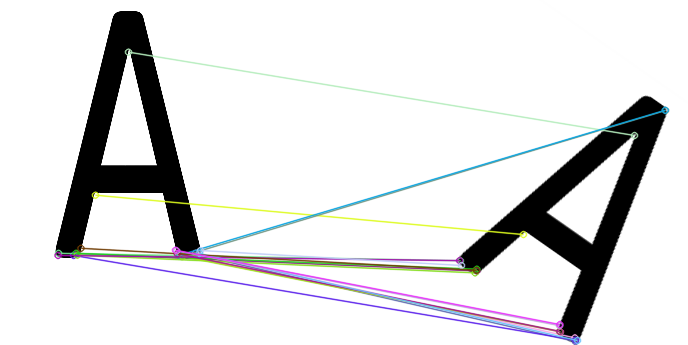
\includegraphics[width=5cm]{assets/IT/testing/target_node/orb-a.png}
\caption{Beispielbild mit Erkennungspunkten 'Matches'}
\label{img:orb-example}
\end{figure}

\begin{enumerate}
    \item MIN\_MATCHES\_REQUIRED = 10: Wie viele Matches muss es geben?
    \item MAX\_DISTANCE\_ALLOWED = 50: Wie ungenau dürfen die Matches maximal sein?
    \item Differenz Messpunkte < 5: Differenz der Anzahl Matches für jeden Buchstaben, um die Buchstaben mit den zwei meisten Matches vergleichen zu müssen, anstatt direkt den Buchstaben mit den meisten Matches zu nehmen.
    \item Distanz der Distanz > 5: Differenz in der durchschnittlichen Distanz der Matches der zwei Buchstaben mit den meisten Matches. Hat der Buchstaben mit weniger Matches eine Distanz, die mindestens 6 kleiner ist, passt dieser besser.
\end{enumerate}

Die finalen Werte wurden mithilfe von diesen Testresultaten in Tabelle \ref{letter-matches-orb} ermittelt. Ist die Anzahl Match Differenz grösser als 5, wird die Distanz von zwei Buchstaben gemessen.  Ist die Differenz der Distanzen grösser als 5, wird der zweite Buchstabe genommen. Werden benötigte Anzahl Matches nicht erreicht oder wird die maximale Distanz überschritten, wird kein Buchstabe erkannt.

\begin{table}[H]
\centering
\small
\begin{tabularx}{\textwidth}{|c|X|X|c|X|c|}
\hline
\textbf{Buchstabe} & \textbf{Anzahl Matches pro Buchstabe} & \textbf{Anzahl Match Differenz} & \textbf{Distanz} & \textbf{Differenz Distanz} \\
\hline
None & {'A': 5, 'B': 5, 'C': 5} & 0 &  &  \\
\hline
A & {'A': 135, 'B': 42, 'C': 22} & 93 & A: 0.00 &  \\
\hline
B & {'B': 221, 'C': 51, 'A': 42} & 170 & B: 0.00 &  \\
\hline
C & {'C': 173, 'B': 51, 'A': 22} & 122 & C: 0.00 &  \\
\hline
None & {'B': 11, 'A': 10, 'C': 10} & 1 & B: 72.45, A: 63.30 & \textit{Distanzen > 50}\\
\hline
A & {'A': 21, 'B': 11, 'C': 9} & 10 & A: 18.80 &  \\
\hline
B & {'B': 25, 'A': 12, 'C': 10} & 13 & B: 13.80 &  \\
\hline
B & {'B': 28, 'A': 21, 'C': 15} & 7 & B: 15.70 &  \\
\hline
C & {'A': 24, 'C': 23, 'B': 18} & 1 & A: 45.58, C: 32.61 & 12.97 \\
\hline
C & {'B': 22, 'C': 22, 'A': 13} & 0 & B: 35.41, C: 29.77 & 5.64 \\
\hline
C & {'B': 19, 'C': 15, 'A': 13} & 4 & B: 23.30, c: 29.01 & 5.71 \\
\hline
A & {'A': 26, 'C': 14, 'B': 12} & 12 & A: 22.30 &  \\
\hline
A & {'A': 20, 'B': 13, 'C': 9} & 7 & A: 16.30 &  \\
\hline
A & {'A': 24, 'B': 12, 'C': 10} & 12 & A: 16.10 &  \\
\hline
B & {'B': 28, 'A': 22, 'C': 15} & 6 & B: 15.80 &  \\
\hline
\end{tabularx}
\caption{Analyse der Buchstaben-Matches mit Distanzen}
\label{letter-matches-orb}
\end{table}

\textbf{Funktionalität testen}

Die Logik, um den richtigen Buchstaben zu erkennen beschränkt sich nicht nur auf den \acrshort{orb} Algorithmus. Es wurde selber noch ein Algorithmus implementiert. Grundsätzlich wird der Buchstabe, für den die meisten Matches gefunden wurden, zurückgeben. Jedoch ist es vor allem bei dem Buchstaben C so, dass es relativ wenige Messpunkte gibt, da der Buchstaben sehr simpel ist. Das heisst, wenn C erkannt werden soll, gibt es oft falsche Buchstaben, mit mehr Messpunkten. Falls die Buchstaben mit den meisten und den zweit meisten Messpunkten nur 5 Messpunkte auseinander liegen, werden die Distanzen der Messpunkte verglichen. Wenn der Buchstaben, der maximal 5 Messpunkte weniger hat, eine durchschnittliche Distanz von mehr als 5 hat, wird der Buchstaben zurückgegeben, mit den wenigeren Messpunkten. Diese Logik wird in den Unittests getestet.

Die folgenden Fälle wurden getestet:

\begin{enumerate}
    \item Buchstabe A ist ersichtlich (verschiedene Rotationen): Optimale Verhältnisse \& realistische Verhältnisse.
    \item Buchstabe B ist ersichtlich (verschiedene Rotationen): Optimale Verhältnisse \& realistische Verhältnisse.
    \item Buchstabe C ist ersichtlich (verschiedene Rotationen): Optimale Verhältnisse \& realistische Verhältnisse.
    \item Kein Buchstabe ist ersichtlich: Optimale Verhältnisse \& realistische Verhältnisse.
\end{enumerate}

\begin{table}[H]
\centering
\small
\begin{tabularx}\textwidth{ |c |X |  X | c | }
\hline
 \textbf{Bild} & \textbf{Soll} & \textbf{Ist} & \textbf{Resultat} \\
  
  \hline

       
\begin{minipage}{.1\textwidth}

\includegraphics[width=\linewidth]{assets/IT/testing/target_node/empty-node.png}
\end{minipage}
        &Kein Buchstabe erkannt.&Kein Buchstabe erkannt.&Erfüllt\\

        \hline

        
       
\begin{minipage}{.1\textwidth}

\includegraphics[width=\linewidth]{assets/IT/testing/target_node/letter-A.png}
\end{minipage}
        &Buchstabe A erkannt.&Buchstabe A erkannt.&Erfüllt\\

        \hline


        
       
\begin{minipage}{.1\textwidth}

\includegraphics[width=\linewidth]{assets/IT/testing/target_node/letter-B.png}
\end{minipage}
        &Buchstabe B erkannt.&Buchstabe B erkannt.&Erfüllt\\

        \hline

        
       
\begin{minipage}{.1\textwidth}

\includegraphics[width=\linewidth]{assets/IT/testing/target_node/letter-C.png}
\end{minipage}
        &Buchstabe C erkannt.&Buchstabe C erkannt.&Erfüllt\\

        \hline

\begin{minipage}{.1\textwidth}
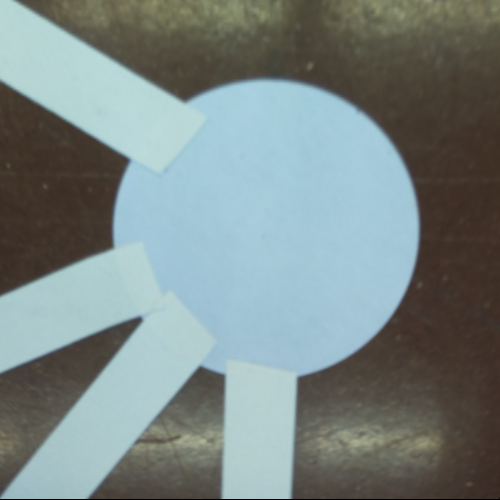
\includegraphics[width=\linewidth]{assets/IT/testing/target_node/node_after_transformation.png}
\end{minipage}
        &Kein Buchstabe erkannt.&Kein Buchstabe erkannt.&Erfüllt\\
        \hline
\begin{minipage}{.1\textwidth}
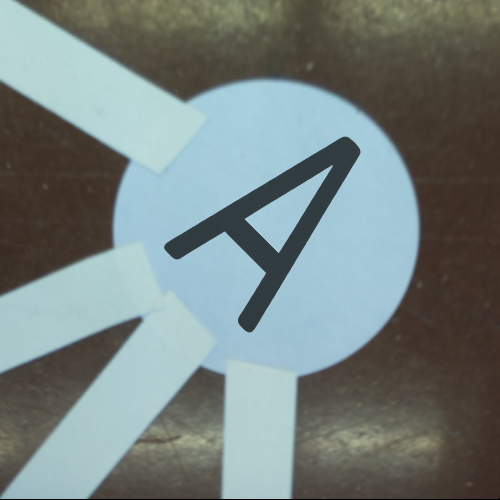
\includegraphics[width=\linewidth]{assets/IT/testing/target_node/real-a.png}
\end{minipage}
        &Buchstabe A erkannt.&Buchstabe A erkannt.&Erfüllt\\

  \hline
\begin{minipage}{.1\textwidth}
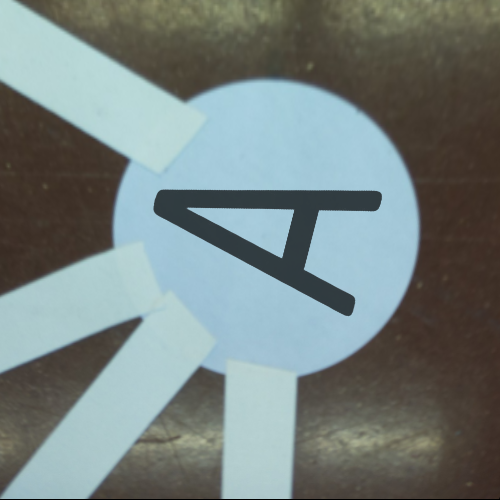
\includegraphics[width=\linewidth]{assets/IT/testing/target_node/real-a2.png}
\end{minipage}
        &Buchstabe A erkannt.&Buchstabe A erkannt.&Erfüllt\\

  \hline
\begin{minipage}{.1\textwidth}
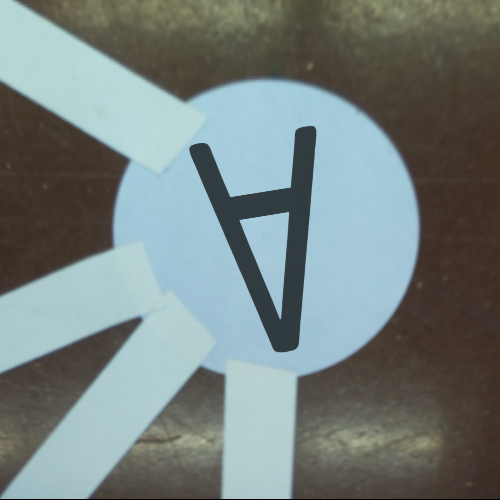
\includegraphics[width=\linewidth]{assets/IT/testing/target_node/real-a3.png}
\end{minipage}
        &Buchstabe A erkannt.&Buchstabe A erkannt.&Erfüllt\\

  \hline

  \begin{minipage}{.1\textwidth}
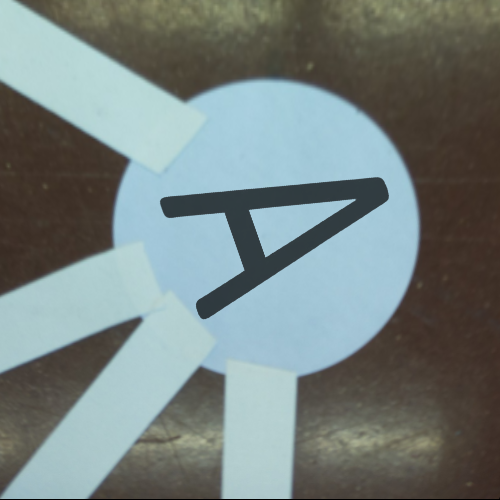
\includegraphics[width=\linewidth]{assets/IT/testing/target_node/real-a4.png}
\end{minipage}
        &Buchstabe A erkannt.&Buchstabe A erkannt.&Erfüllt\\
        \hline

  \begin{minipage}{.1\textwidth}
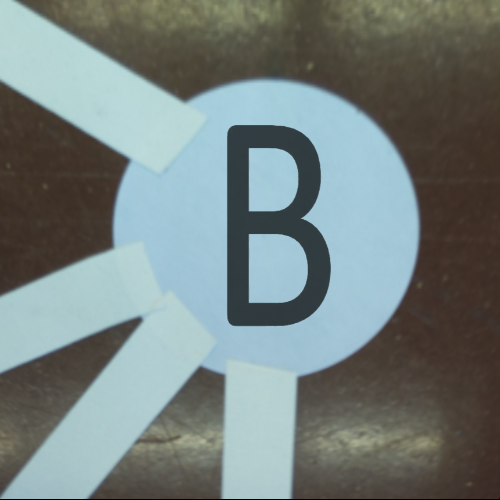
\includegraphics[width=\linewidth]{assets/IT/testing/target_node/real-b.png}
\end{minipage}
        &Buchstabe B erkannt.&Buchstabe B erkannt.&Erfüllt\\
        \hline
          \begin{minipage}{.1\textwidth}
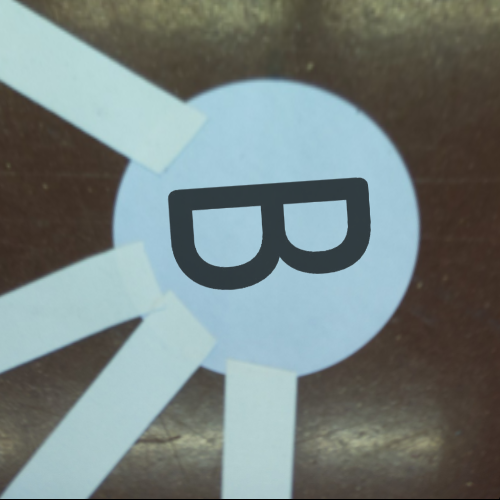
\includegraphics[width=\linewidth]{assets/IT/testing/target_node/real-b2.png}
\end{minipage}
        &Buchstabe B erkannt.&Buchstabe B erkannt.&Erfüllt\\
        \hline
          \begin{minipage}{.1\textwidth}
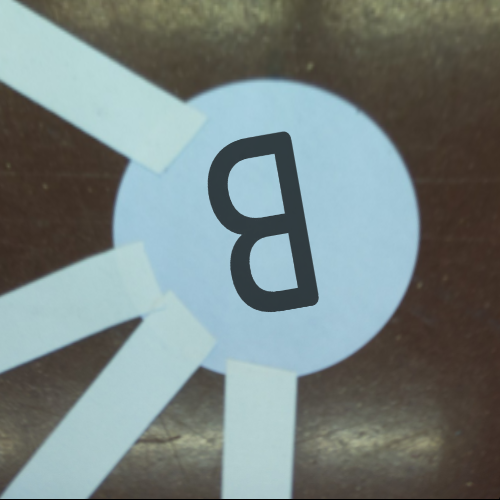
\includegraphics[width=\linewidth]{assets/IT/testing/target_node/real-b3.png}
\end{minipage}
        &Buchstabe B erkannt.&Buchstabe B erkannt.&Erfüllt\\
        \hline
         \end{tabularx}
\end{table}

\newpage

\begin{table}[H]
\centering
\small
\begin{tabularx}\textwidth{| c |X | X | c | }
\hline
 \textbf{Bild} & \textbf{Soll} & \textbf{Ist} & \textbf{Resultat} \\
  
  \hline
          \begin{minipage}{.1\textwidth}
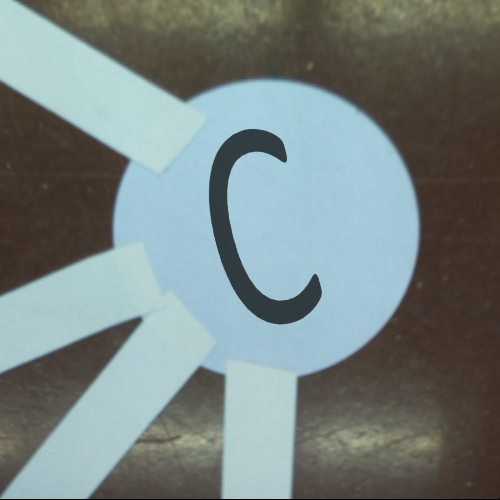
\includegraphics[width=\linewidth]{assets/IT/testing/target_node/real-c.png}
\end{minipage}
        &Buchstabe C erkannt.&Buchstabe C erkannt.&Erfüllt\\

  \hline

            \begin{minipage}{.1\textwidth}
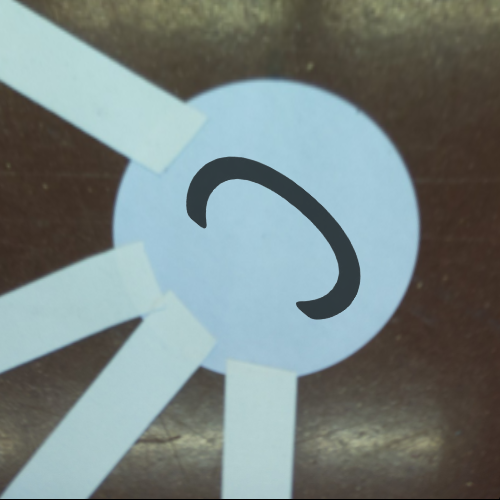
\includegraphics[width=\linewidth]{assets/IT/testing/target_node/real-c2.png}
\end{minipage}
        &Buchstabe C erkannt.&Buchstabe C erkannt.&Erfüllt\\

  \hline

            \begin{minipage}{.1\textwidth}
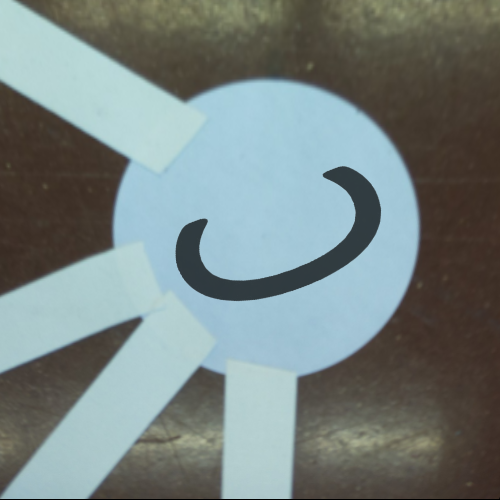
\includegraphics[width=\linewidth]{assets/IT/testing/target_node/real-c3.png}
\end{minipage}
        &Buchstabe C erkannt.&Buchstabe C erkannt.&Erfüllt\\

  \hline
\end{tabularx}
\caption{Target Node Recognition Testprotokoll}
\label{table:target-node-test}
\end{table}



Auf dem folgenden Bild \ref{img:target_node_unittests} sind alle Unittests ersichtlich, die alle erfolgreich waren.

\begin{figure}[H]
\centering
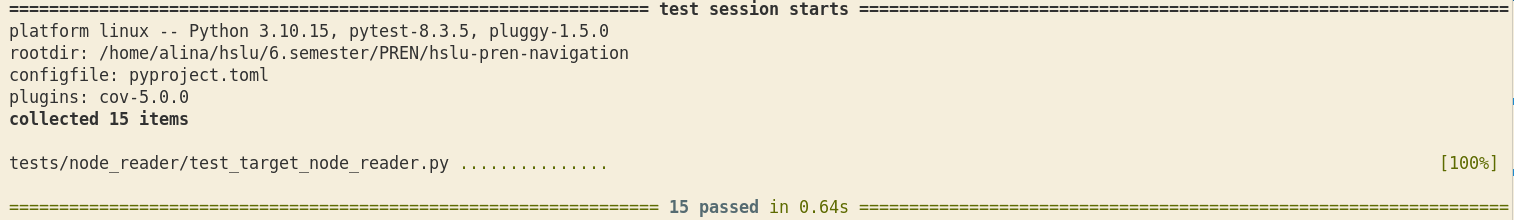
\includegraphics[width=\textwidth]{assets/IT/testing/target_node/target_node_reader_unittests.png}
\caption{Alle Target Node Unittests}
\label{img:target_node_unittests}
\end{figure}

%%%%%%%%%%%%%%%%%%%%%%%%%%%% Unittests %%%%%%%%%%%%%%%%%%%%%%%%%%%
\newpage
\subsection*{Navigation automatisierte Unittests}\label{nav-unittests}
  \addcontentsline{toc}
    {subsection}
    {Navigation automatisierte Unittests}

\subsubsection*{Angle Reader}\label{angle-reader-unittests}
\addcontentsline{toc}{subsubsection}{Angle Reader}

Der Angle Reader wird verwendet, um aus Kamerabildern Winkel zu erkennen, die den Positionen und Verbindungen im Basisgraphen entsprechen. Er nutzt dazu Bildverarbeitung, um Knoten zu maskieren, Konturen zu analysieren, Winkel zu berechnen und diese anschliessend den Verbindungen zuzuordnen. Die folgenden Unittests prüfen das Verhalten einzelner Teilfunktionen unabhängig vom realen Bildinput.

Folgende Szenarien wurden getestet:

\begin{enumerate}
\item Maske korrekt vorbereiten aus RGB-Bild (HSV-Filterung).
\item Knotenmaskierung mit Morphologie und Kreiszeichnung.
\item Winkelberechnung aus erkannter Kontur.
\item Ergebnisbild speichern, wenn Winkel vorhanden sind.
\item Fehler beim Speichern ohne berechnete Winkel.
\item Für jedes gültige Knotenpaar: Korrekte relative Winkelberechnung.
\item Für jede Verbindung: Zuordnung eines einzelnen Winkels zu einem Nachbarknoten.
\item Für jeden Knoten: Positionsbasierte Winkelzuordnung bei unsortierter Eingabe.
\end{enumerate}

Die Abbildung \ref{fig:angle-reader-unittests} dokumentiert das Resultat der Unittest Session.

\begin{figure}[H]
\centering
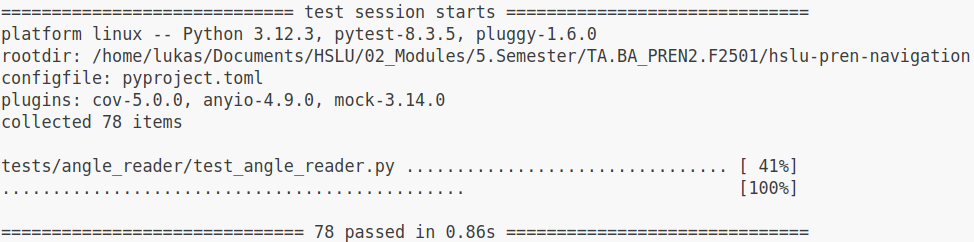
\includegraphics[width=\textwidth]{assets/IT/testing/unittests/angle_reader_unittests_result.png}
\caption{Alle Angle Reader Unittests}
\label{fig:angle-reader-unittests}
\end{figure}


\newpage
\subsubsection*{UART Connector}\label{uart-connector-unittests}
\addcontentsline{toc}{subsubsection}{UART Connector}

Der UART Connector abstrahiert die Kommunikation mit dem Mikrocontroller über eine serielle Schnittstelle. Dabei werden Fahr- und Drehbefehle sowie Signalisierungen wie Hindernismeldungen kodiert und gesendet. Die Rückmeldung erfolgt durch interpretierte Statusbits. Die Unittests überprüfen die korrekte Zusammensetzung der Nachrichten und das Verhalten bei spezifischen Rückgabewerten.

Folgende Szenarien wurden getestet:

\begin{enumerate}
\item Fahrt vorwärts mit Hindernis im Weg (unerwartetes Objekt).
\item Rückwärtsfahrt wird korrekt übermittelt.
\item Drehung nach rechts mit Summenkontrolle der Winkelteile.
\item Drehung nach links und Zuordnung des Richtungsbits.
\item Meldung eines Hindernisses via UART.
\end{enumerate}

Die Abbildung \ref{fig:uart-connector-unittests} zeigt das Resultat der Unittest Session.

\begin{figure}[H]
\centering
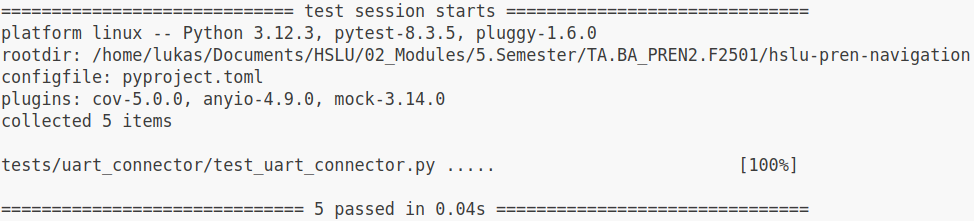
\includegraphics[width=\textwidth]{assets/IT/testing/unittests/uart_connector_unittests_result.png}
\caption{Alle UART Connector Unittests}
\label{fig:uart-connector-unittests}
\end{figure}


\newpage
\subsubsection*{Object Detector}\label{object-detector-unittests}
\addcontentsline{toc}
{subsubsection}
{Object Detector}

Der Object Detector erhaelt Bilder und detektiert, welche Objekte sich darauf befinden mit dem YOLO Model. Dann wird ein Algorithmus angewandt, um sicherzustellen, dass nur das Objekt direkt vor dem Roboter beachtet wird, ausser hinter dem Hindernis befindet sich eine Pylone, dann soll die Pylone beachtet werden.
Die Unittests des Object Detectors sollen nicht primär das Modell testen, sondern den Algorithmus, der das relevante Objekt findet. Folgende Szenarien wurden getestet:

\begin{enumerate}
    \item Eine Barriere befindet sich vor dem Roboter, dahinter ein Knoten.
    \item Nur ein Knoten befindet sich vor dem Roboter.
    \item Nur eine Pylone befindet sich vor dem Roboter (auf dem nächsten Knoten).
    \item Eine Barriere befindet sich vor dem Roboter, dahinter eine Pylone.
    \item Eine Barriere befindet sich vor dem Roboter, dahinter ein Knoten. Ebenfalls ist auf dem Bild eine Barriere, die nicht direkt vor dem Roboter ist.
    \item Ein Knoten befindet sich vor dem Roboter. Auf der Linie zu der Seite, befindet sich eine Barriere, die nicht vor dem Roboter ist.
\end{enumerate}

\textit{Die annotierten Bilder in der folgenden Tabelle \ref{table:object-det-test}, wurden von dem Object Detector selber annotiert in dem jeweiligen Testfall.}

\begin{table}[H]
\centering
\small
\begin{tabularx}\textwidth{|c | X |X | X | X | c | }
\hline
  \textbf{Nr} & \textbf{Bild} & \textbf{Annotiertes Bild} &\textbf{Soll} & \textbf{Ist} & \textbf{Resultat} \\
  
  \hline

        1&
\begin{minipage}{.18\textwidth}
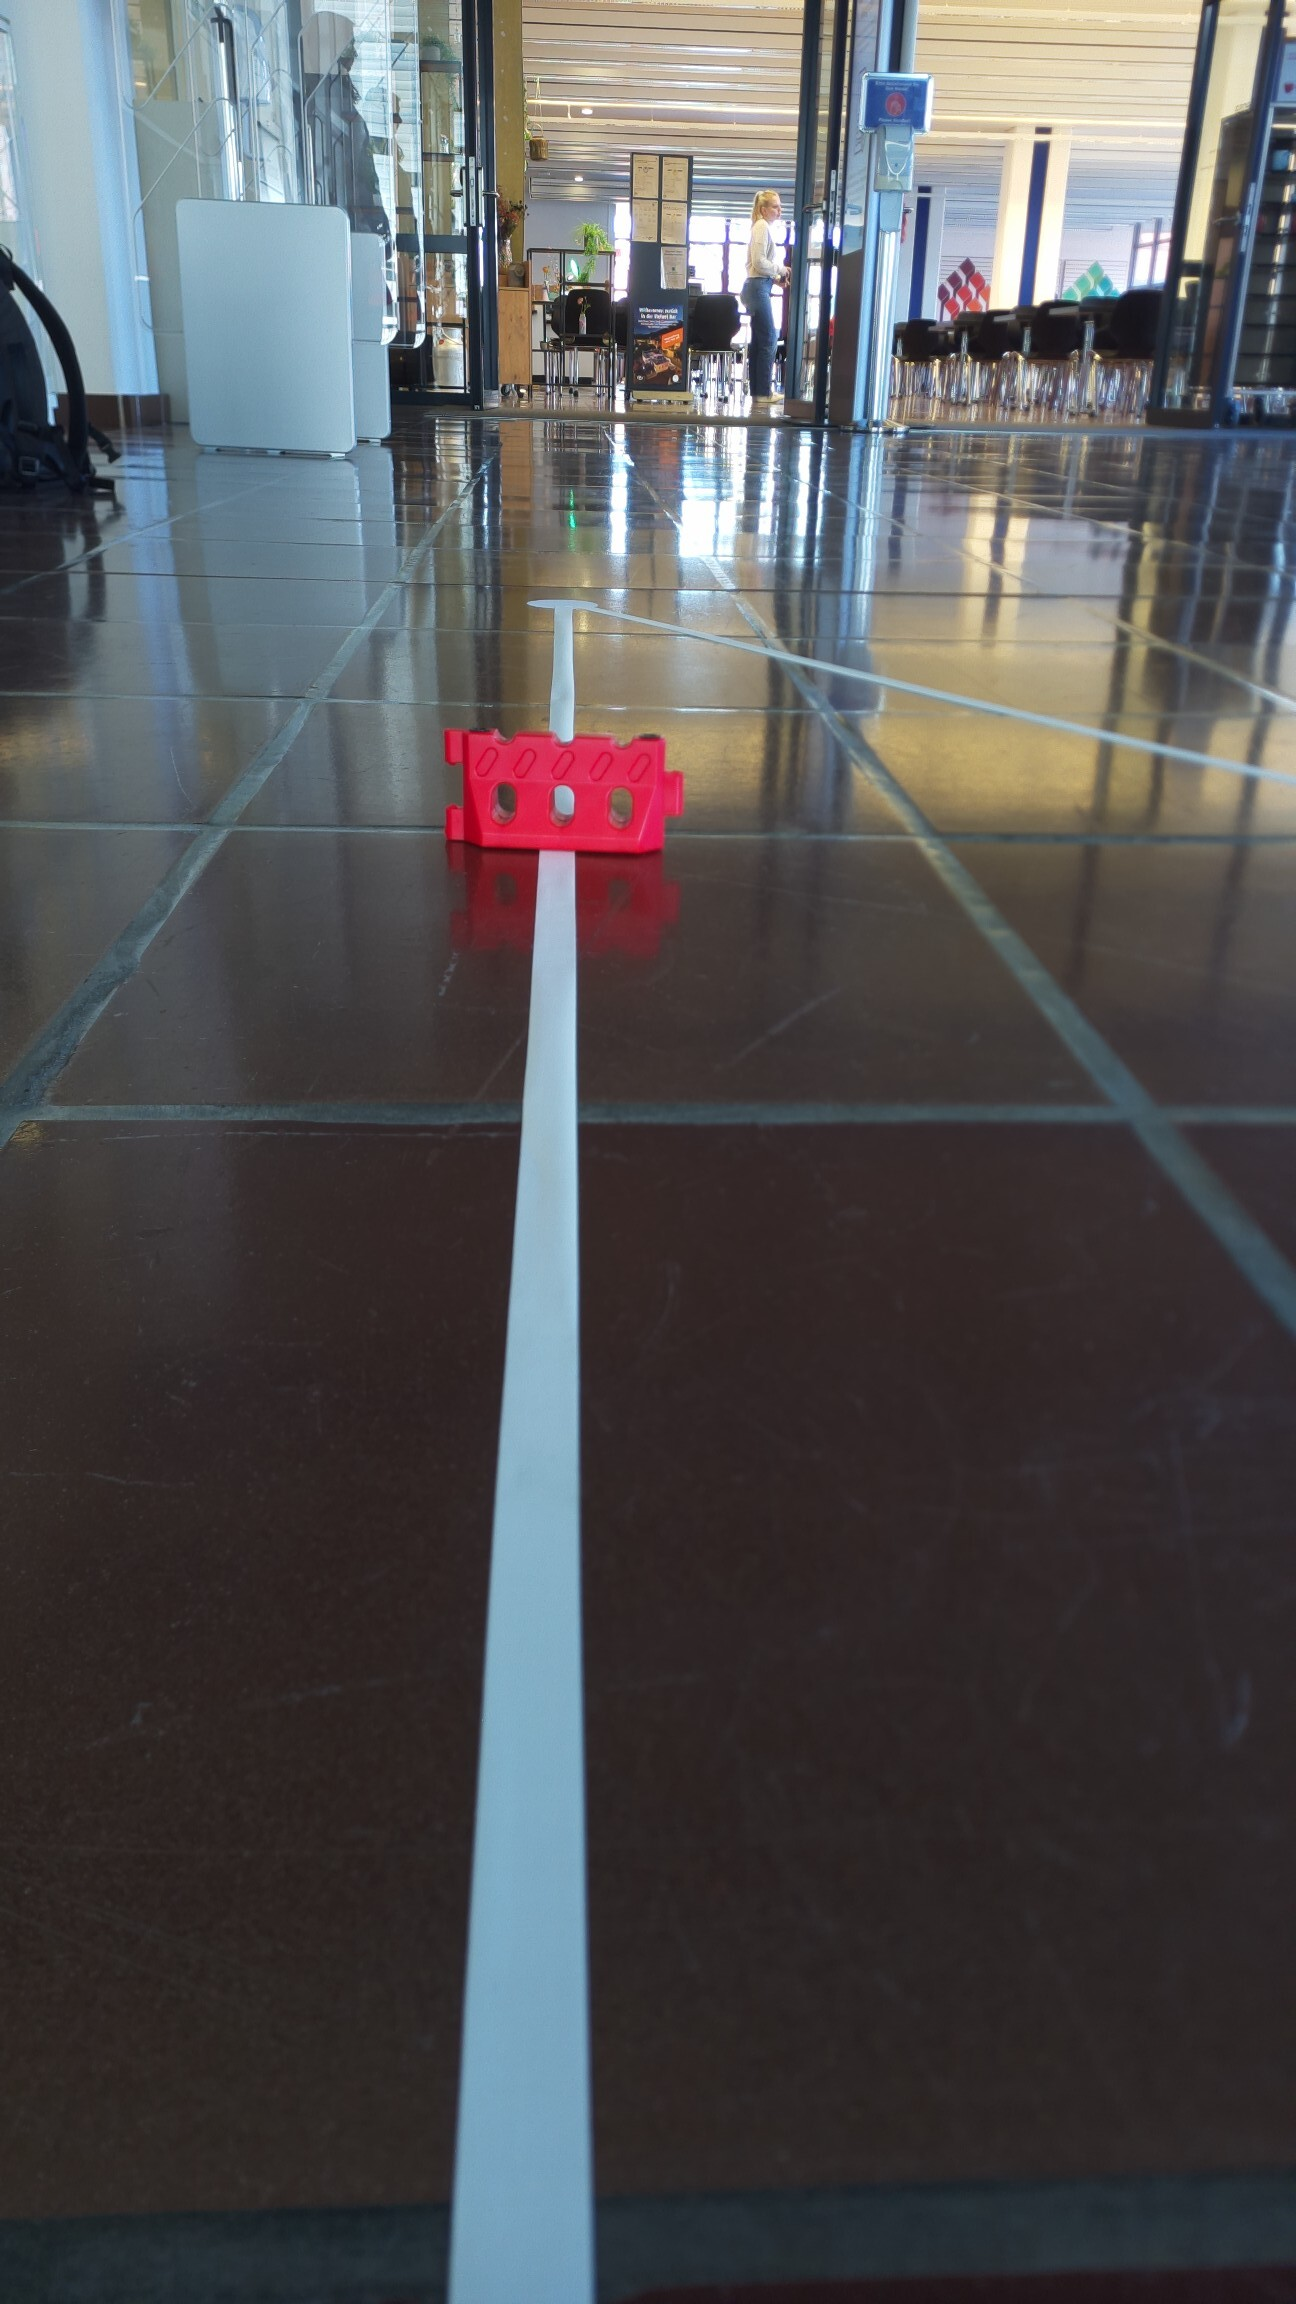
\includegraphics[width=\linewidth]{assets/IT/testing/yolo/barrier.jpg}
\end{minipage}
        &
\begin{minipage}{.18\textwidth}
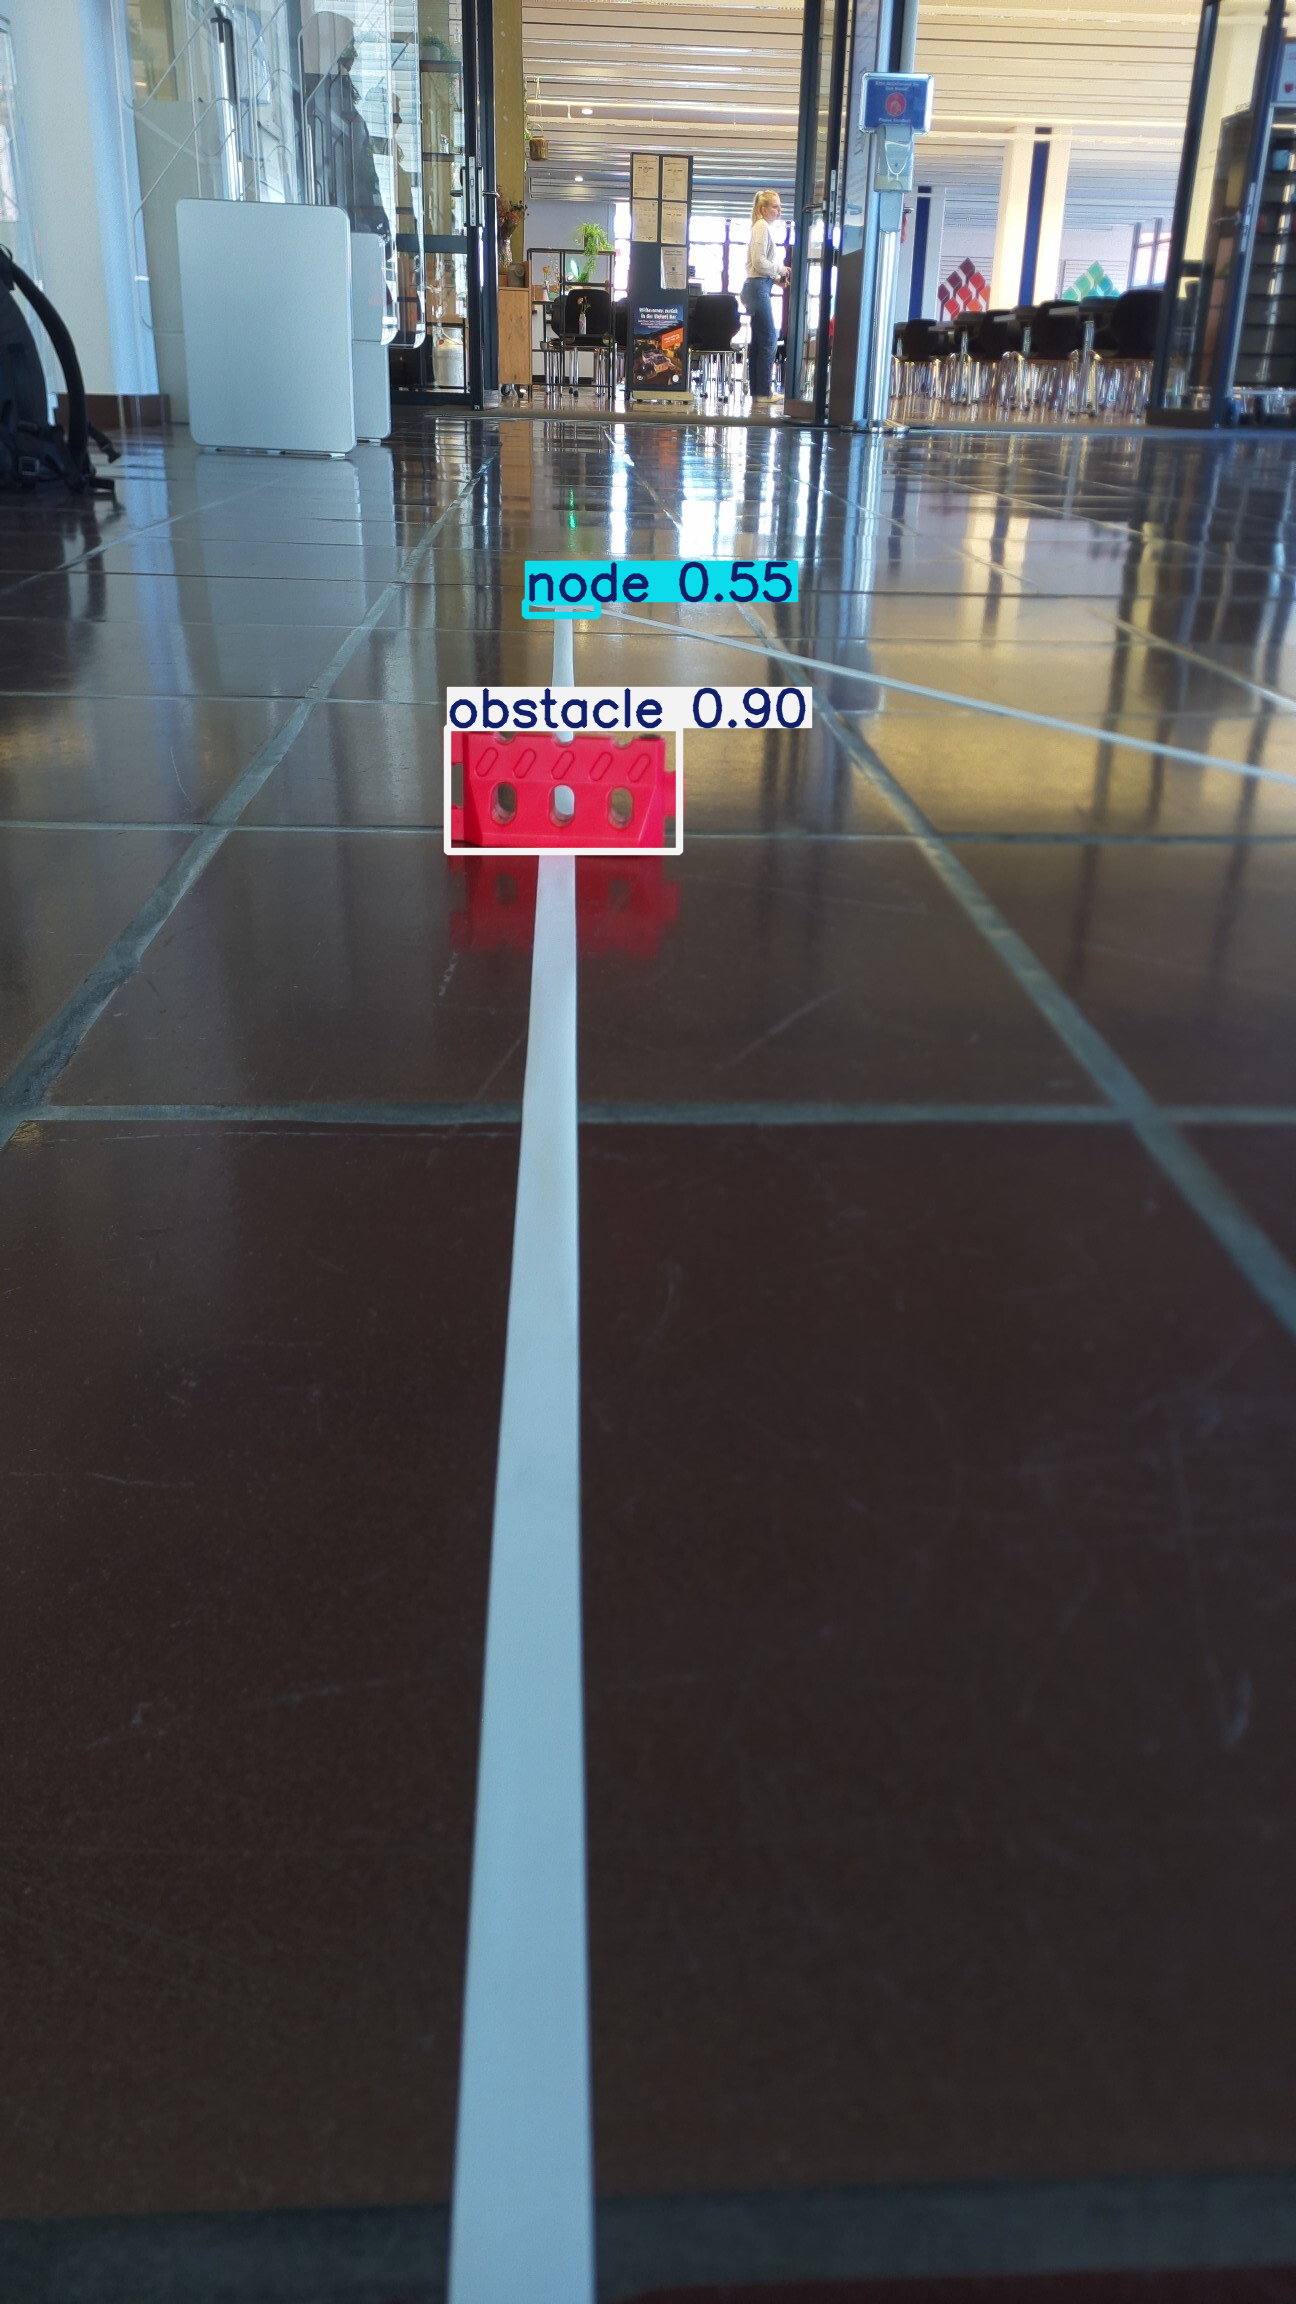
\includegraphics[width=\linewidth]{assets/IT/testing/yolo/barrier_annot.png}
\end{minipage}        
        &Barriere erkannt.&Barriere erkannt.& Erfüllt\\
        \hline
        2&
\begin{minipage}{.18\textwidth}
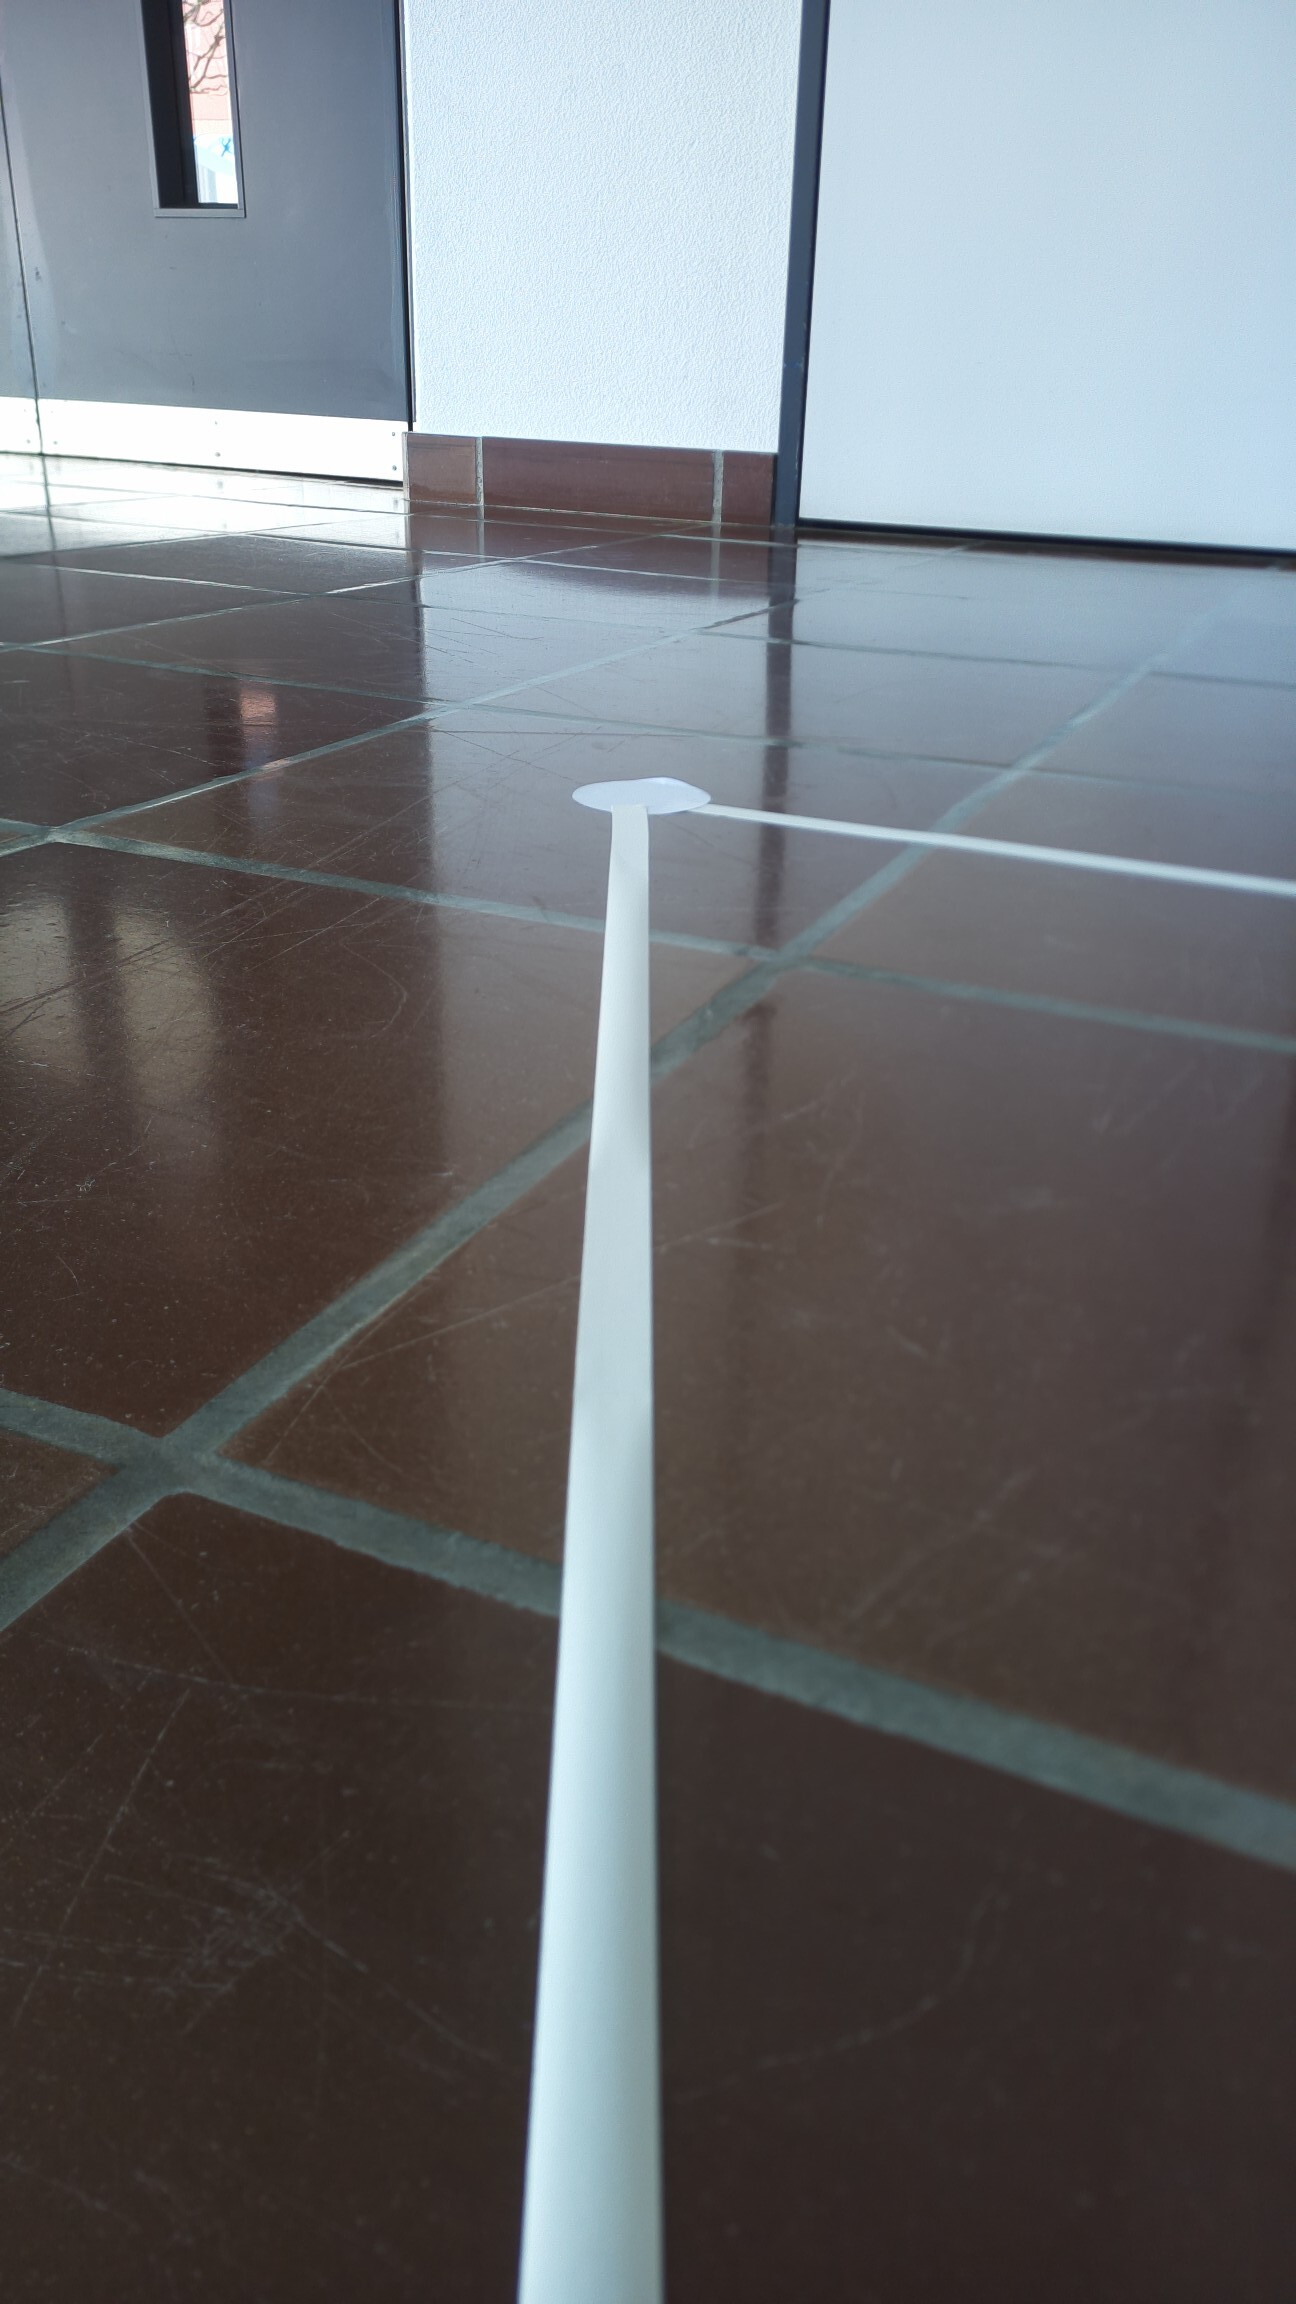
\includegraphics[width=\linewidth]{assets/IT/testing/yolo/node.jpg}
\end{minipage}
        &
\begin{minipage}{.18\textwidth}
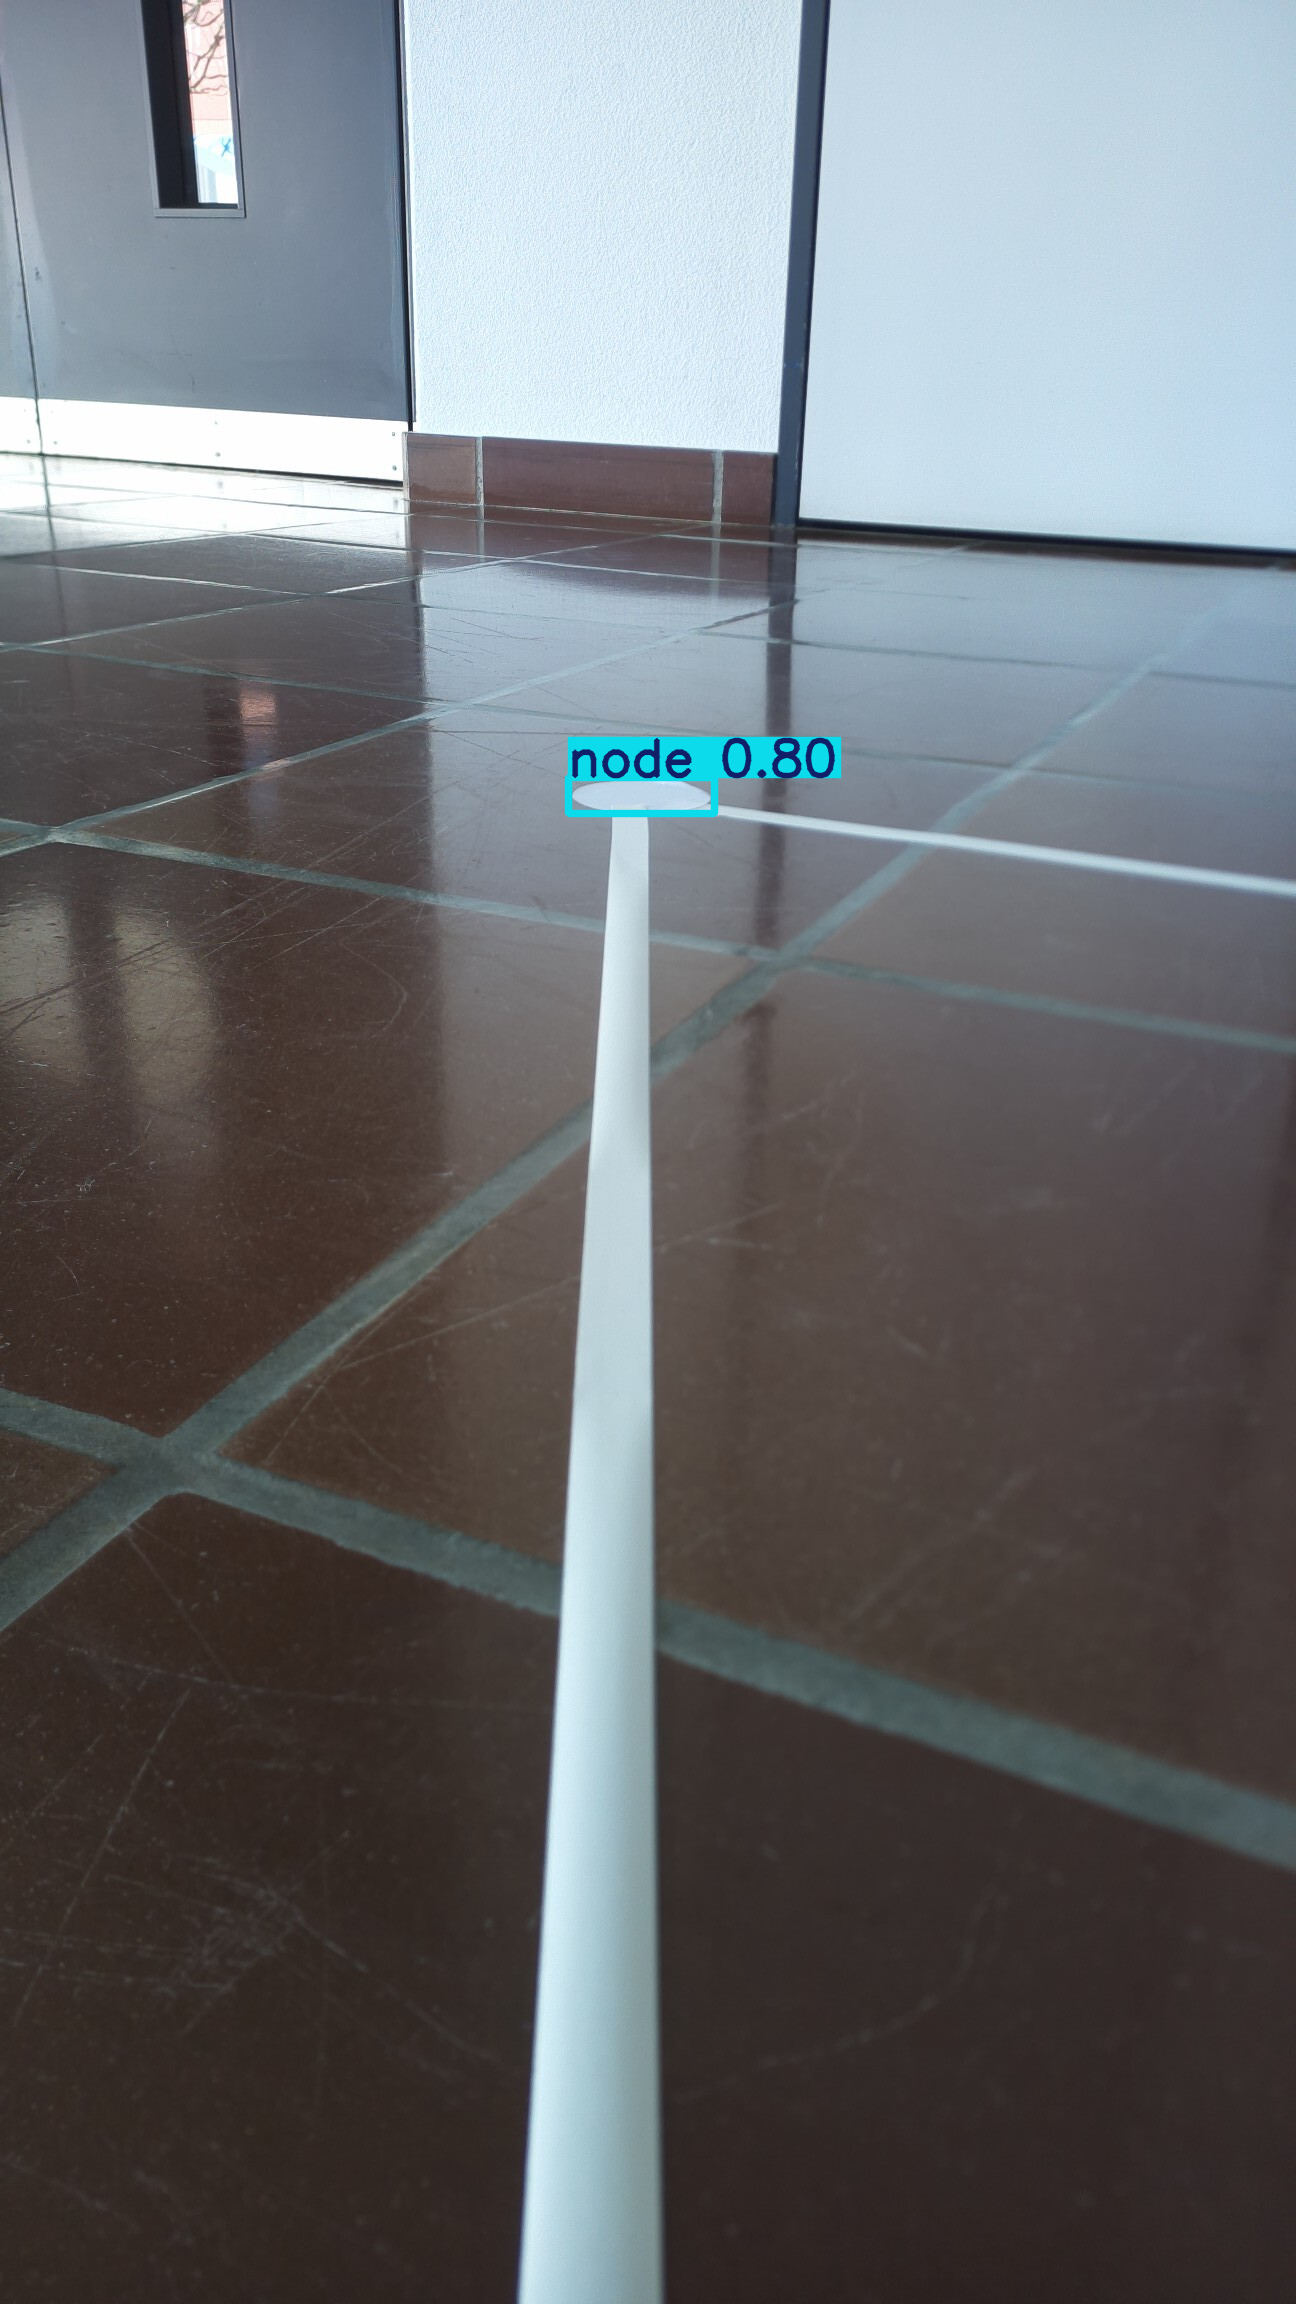
\includegraphics[width=\linewidth]{assets/IT/testing/yolo/node_annot.png}
\end{minipage}        
        &Knoten erkannt.&Knoten erkannt.& Erfüllt\\
        \hline

        3&
\begin{minipage}{.18\textwidth}
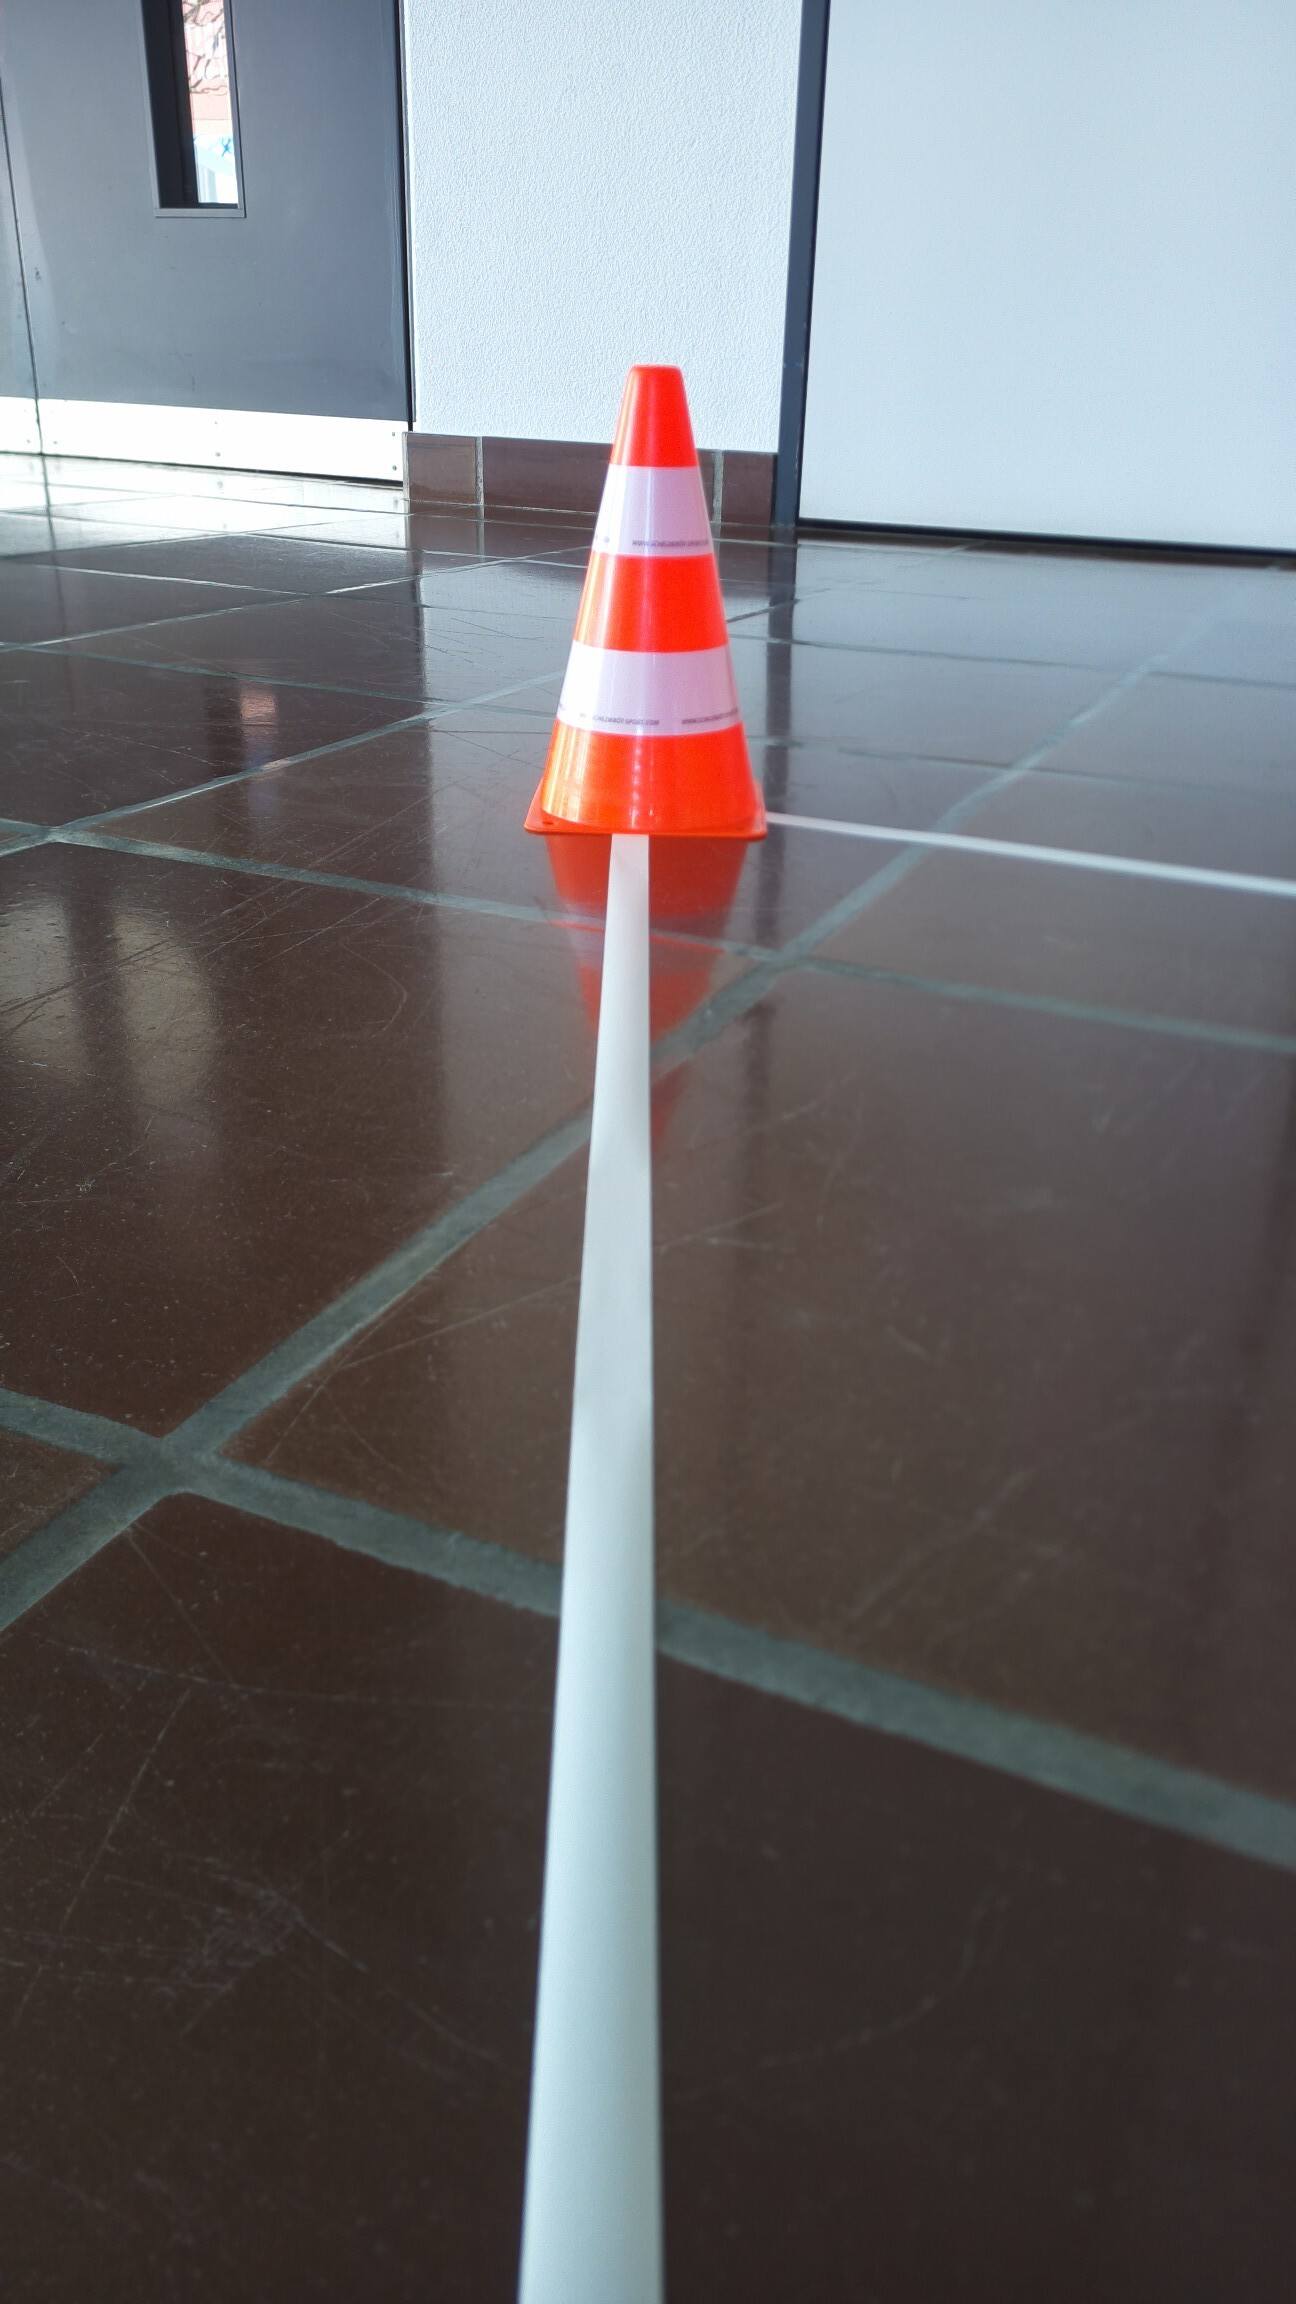
\includegraphics[width=\linewidth]{assets/IT/testing/yolo/pylon.jpg}
\end{minipage}
        &
\begin{minipage}{.18\textwidth}
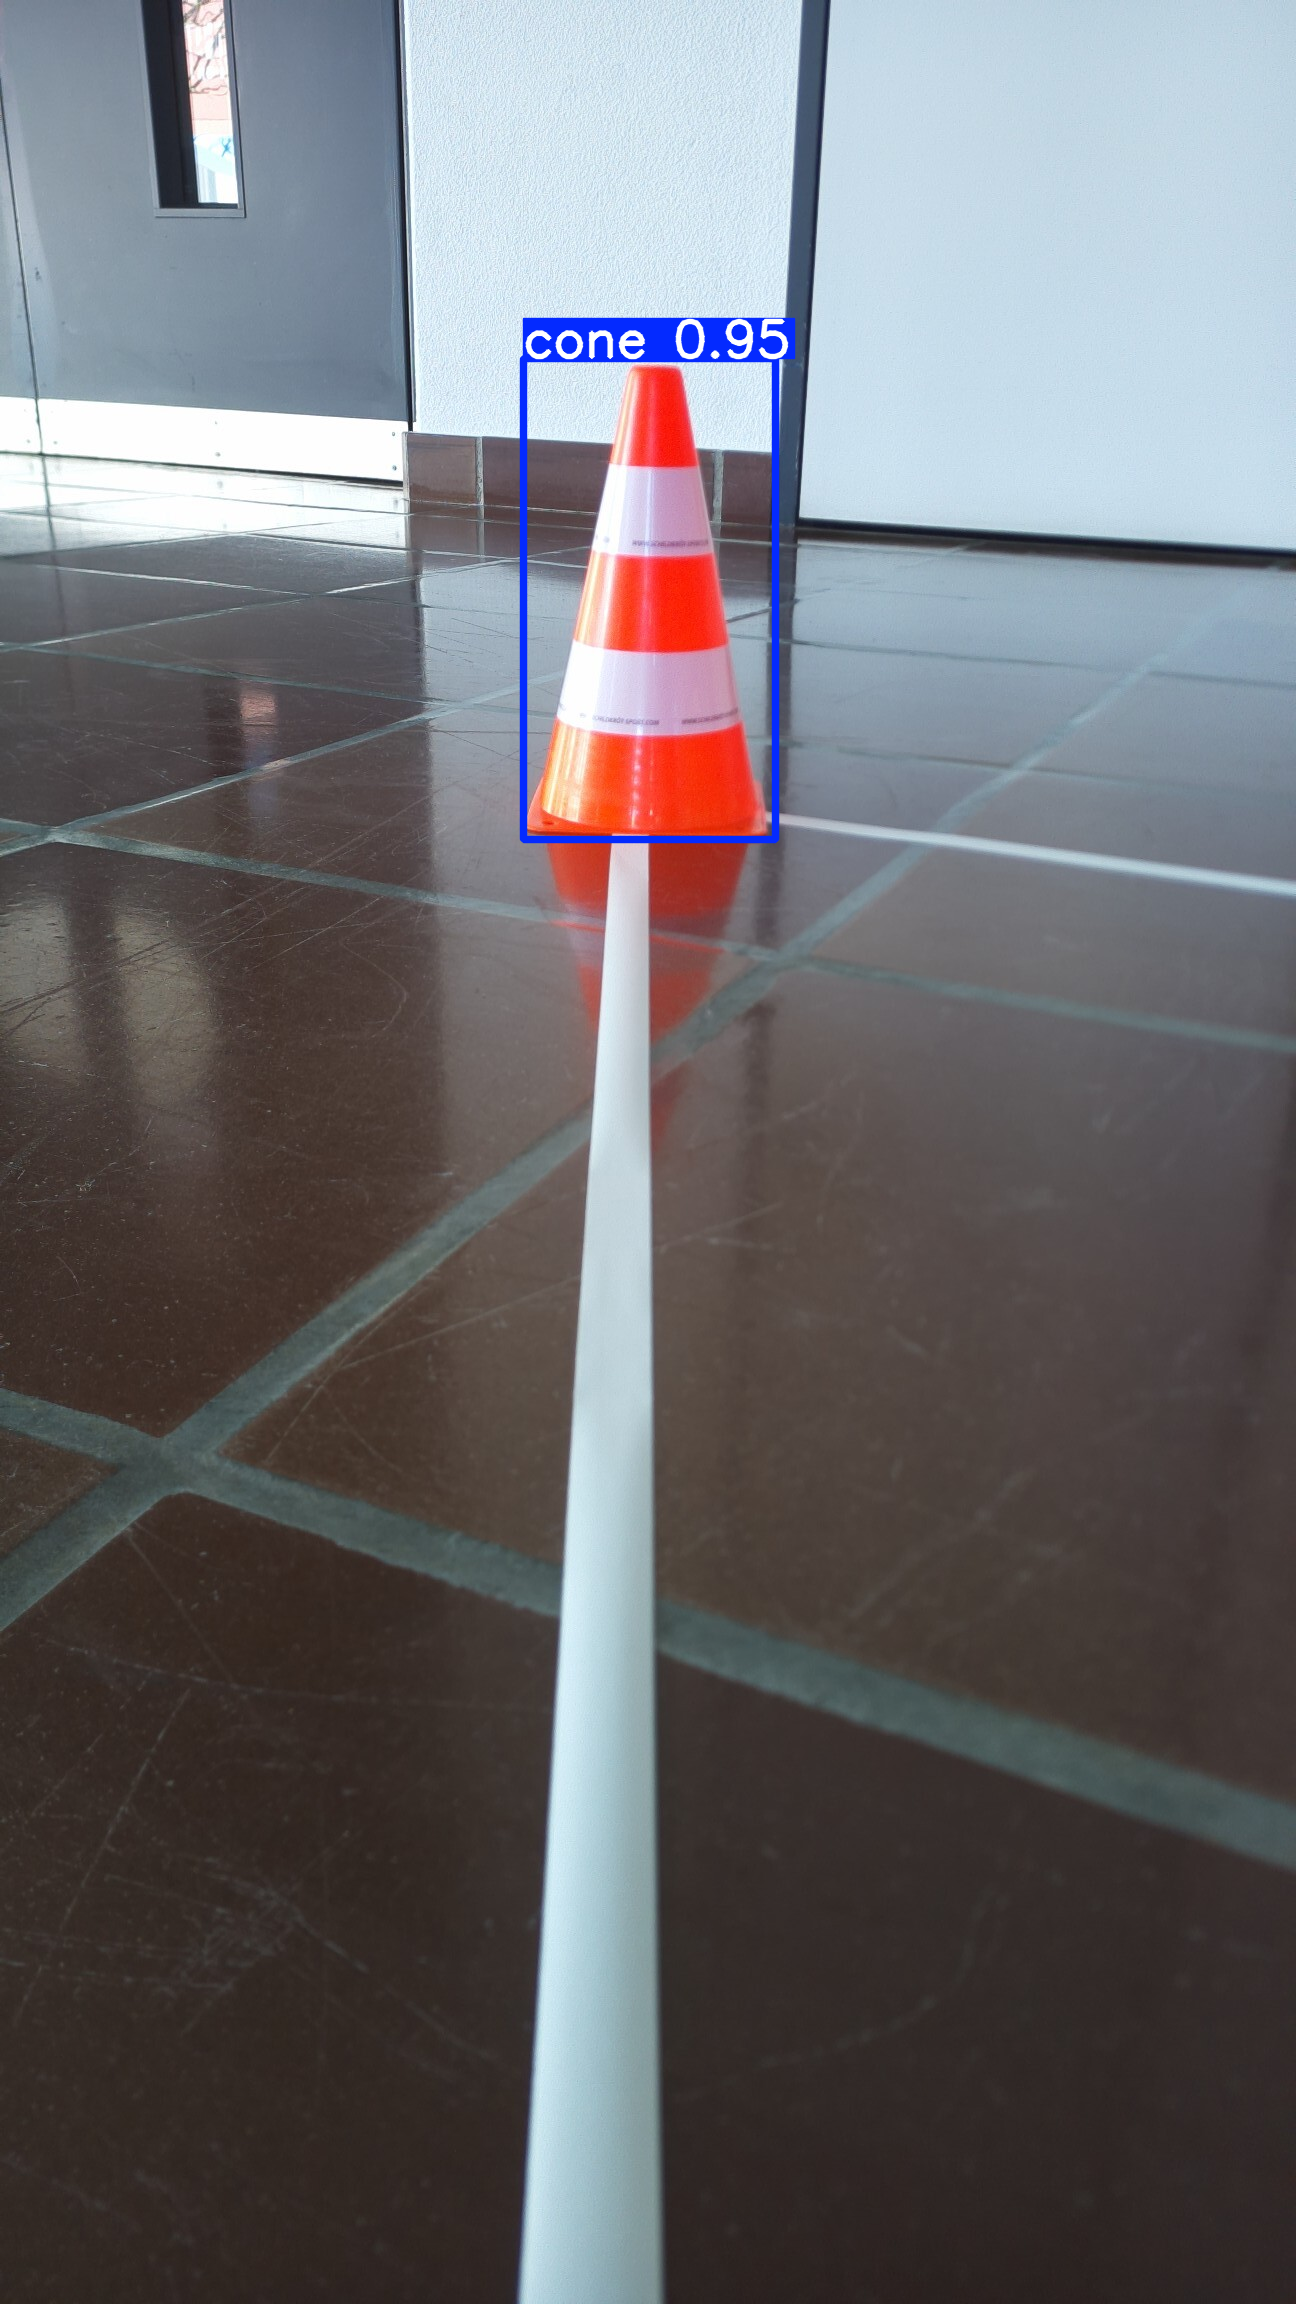
\includegraphics[width=\linewidth]{assets/IT/testing/yolo/pylon_annot.png}
\end{minipage}        
        &Pylone erkannt.&Pylone erkannt.& Erfüllt\\
        \hline


        4&
\begin{minipage}{.18\textwidth}
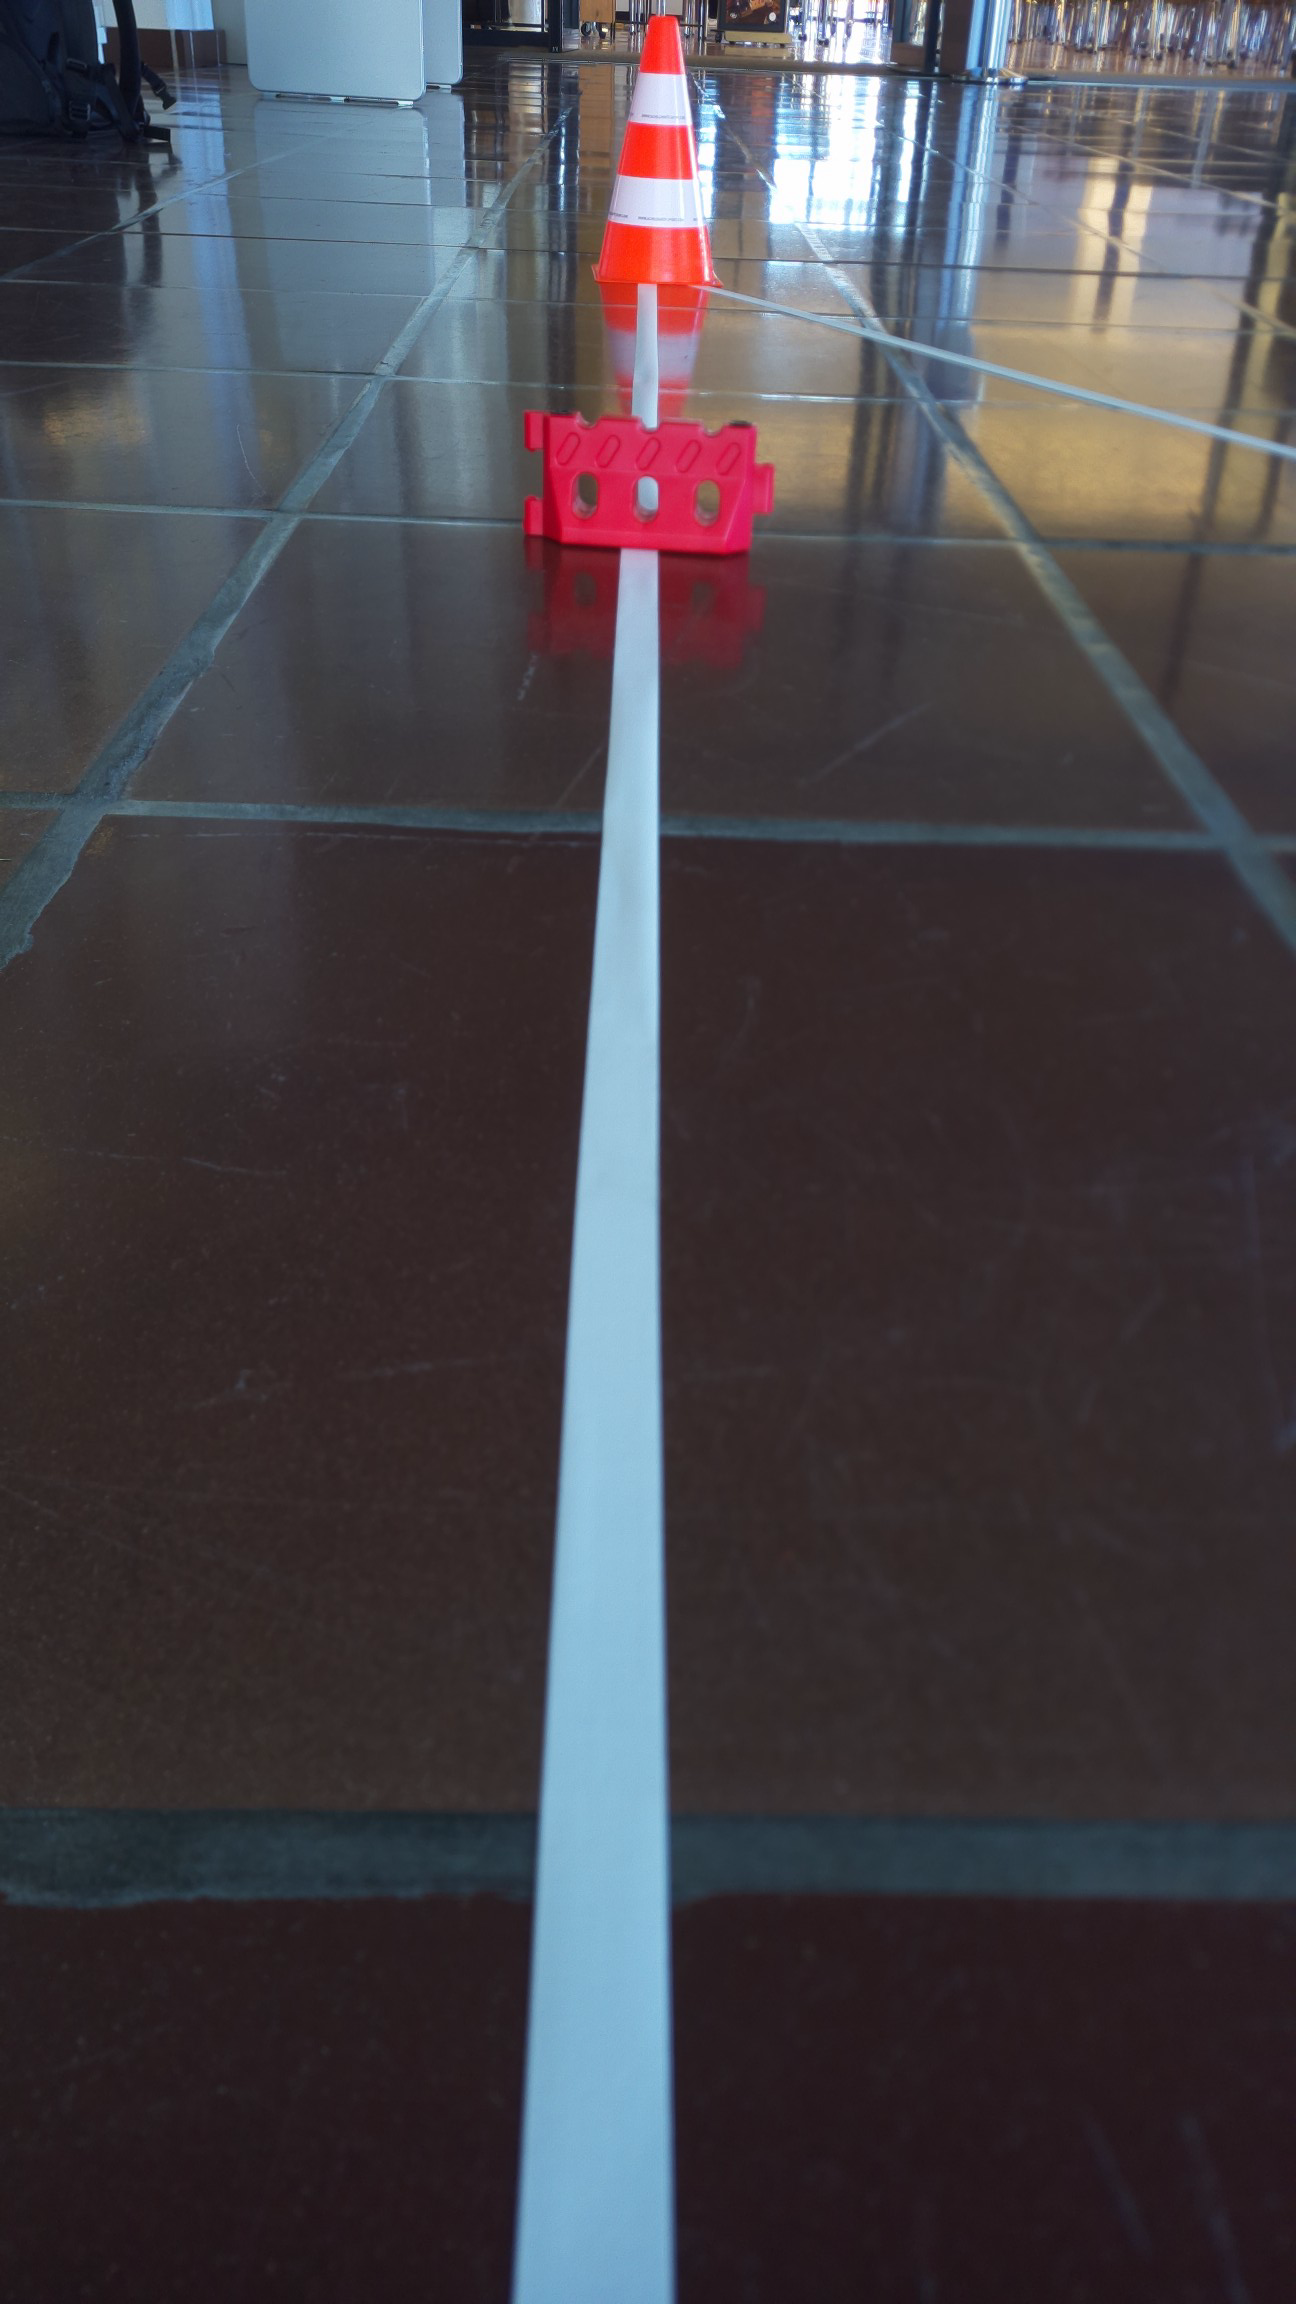
\includegraphics[width=\linewidth]{assets/IT/testing/yolo/pylon_behind_obst.png}
\end{minipage}
        &
\begin{minipage}{.18\textwidth}
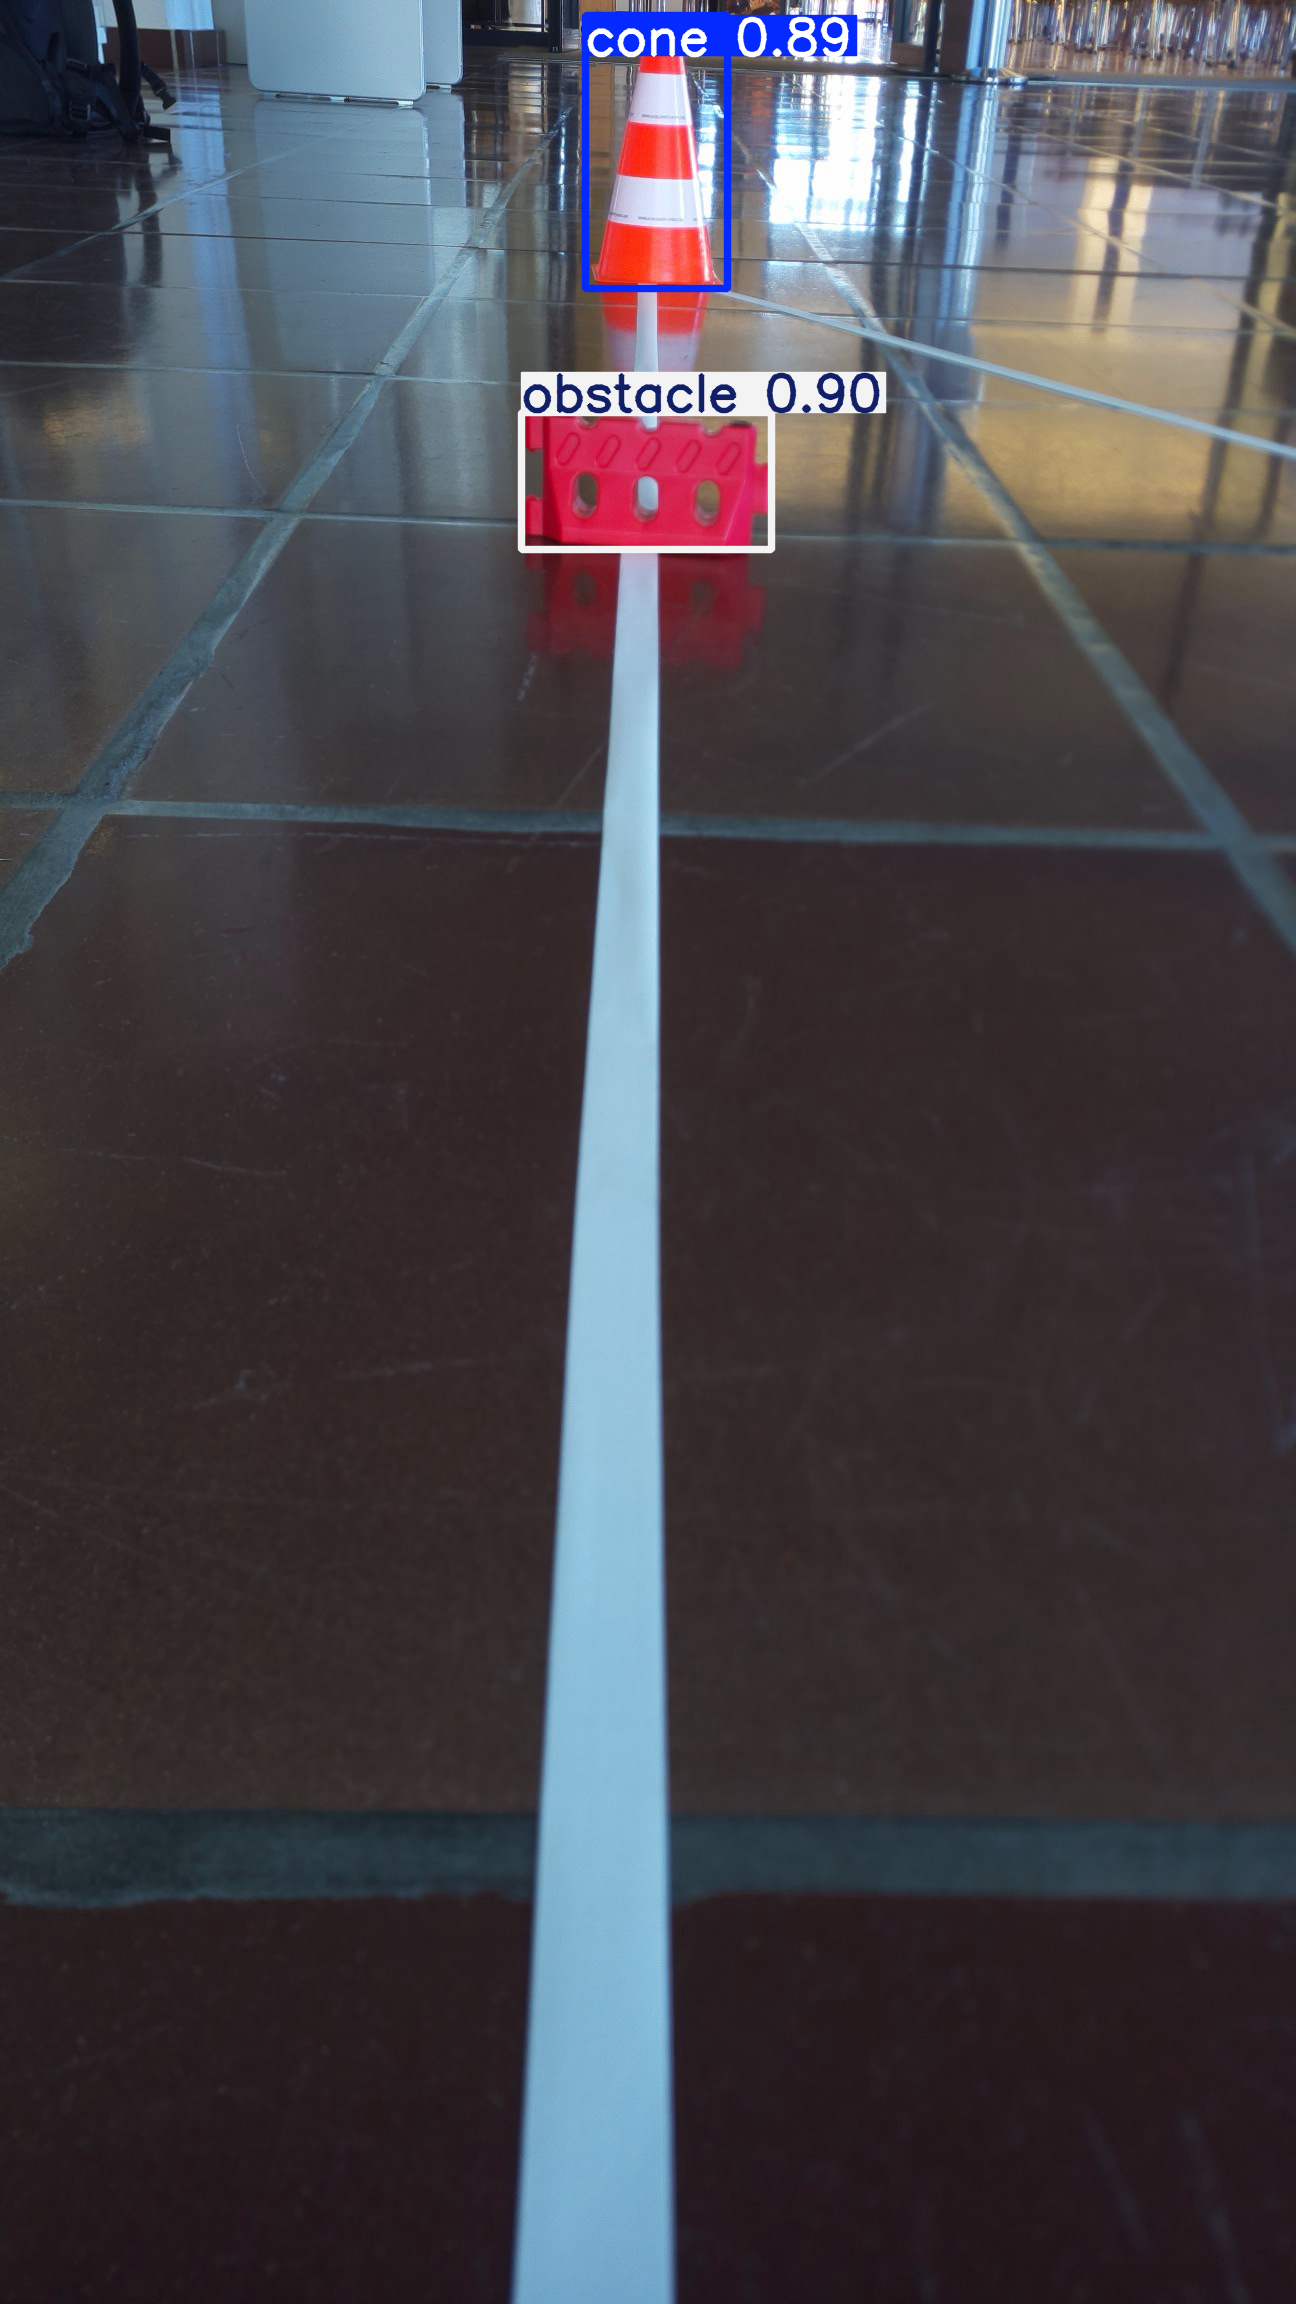
\includegraphics[width=\linewidth]{assets/IT/testing/yolo/pylon_behind_obst_annot.png}
\end{minipage}        
        &Pylone erkannt.&Pylone erkannt.& Erfüllt\\
        \hline

         \end{tabularx}
\end{table}

\newpage

\begin{table}[H]
\centering
\small
\begin{tabularx}\textwidth{|c | X |X | X | X | c | }
\hline
  \textbf{Nr} & \textbf{Bild} & \textbf{Annotiertes Bild} &\textbf{Soll} & \textbf{Ist} & \textbf{Resultat} \\
  \hline
        5&
\begin{minipage}{.18\textwidth}
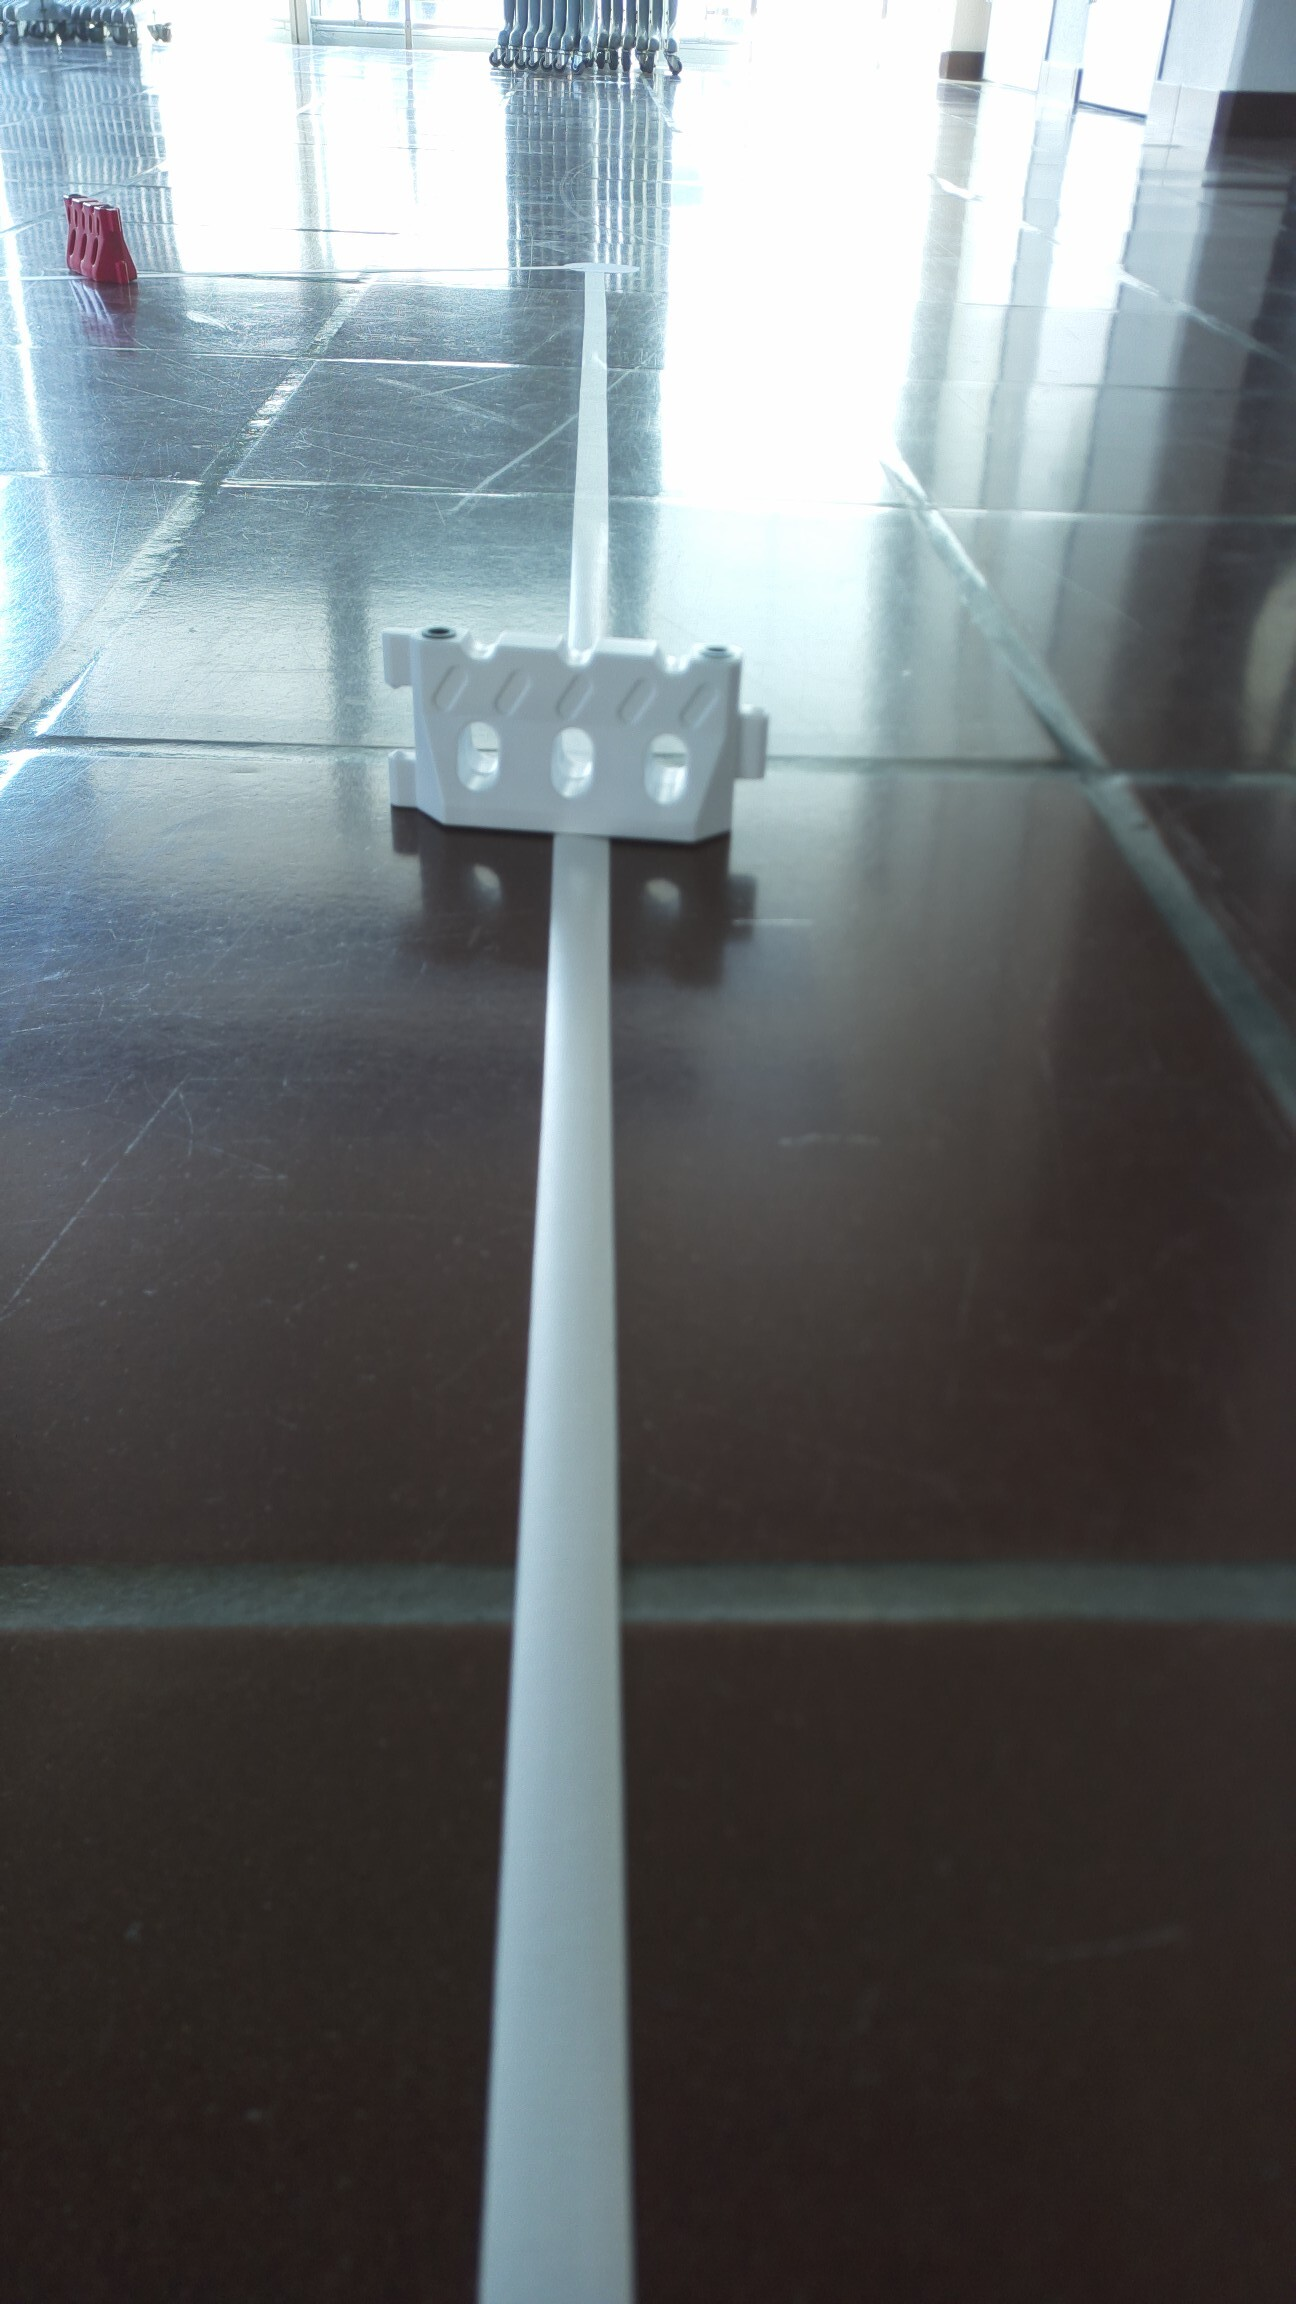
\includegraphics[width=\linewidth]{assets/IT/testing/yolo/2_barriers_1_node.jpg}
\end{minipage}
        &
\begin{minipage}{.18\textwidth}
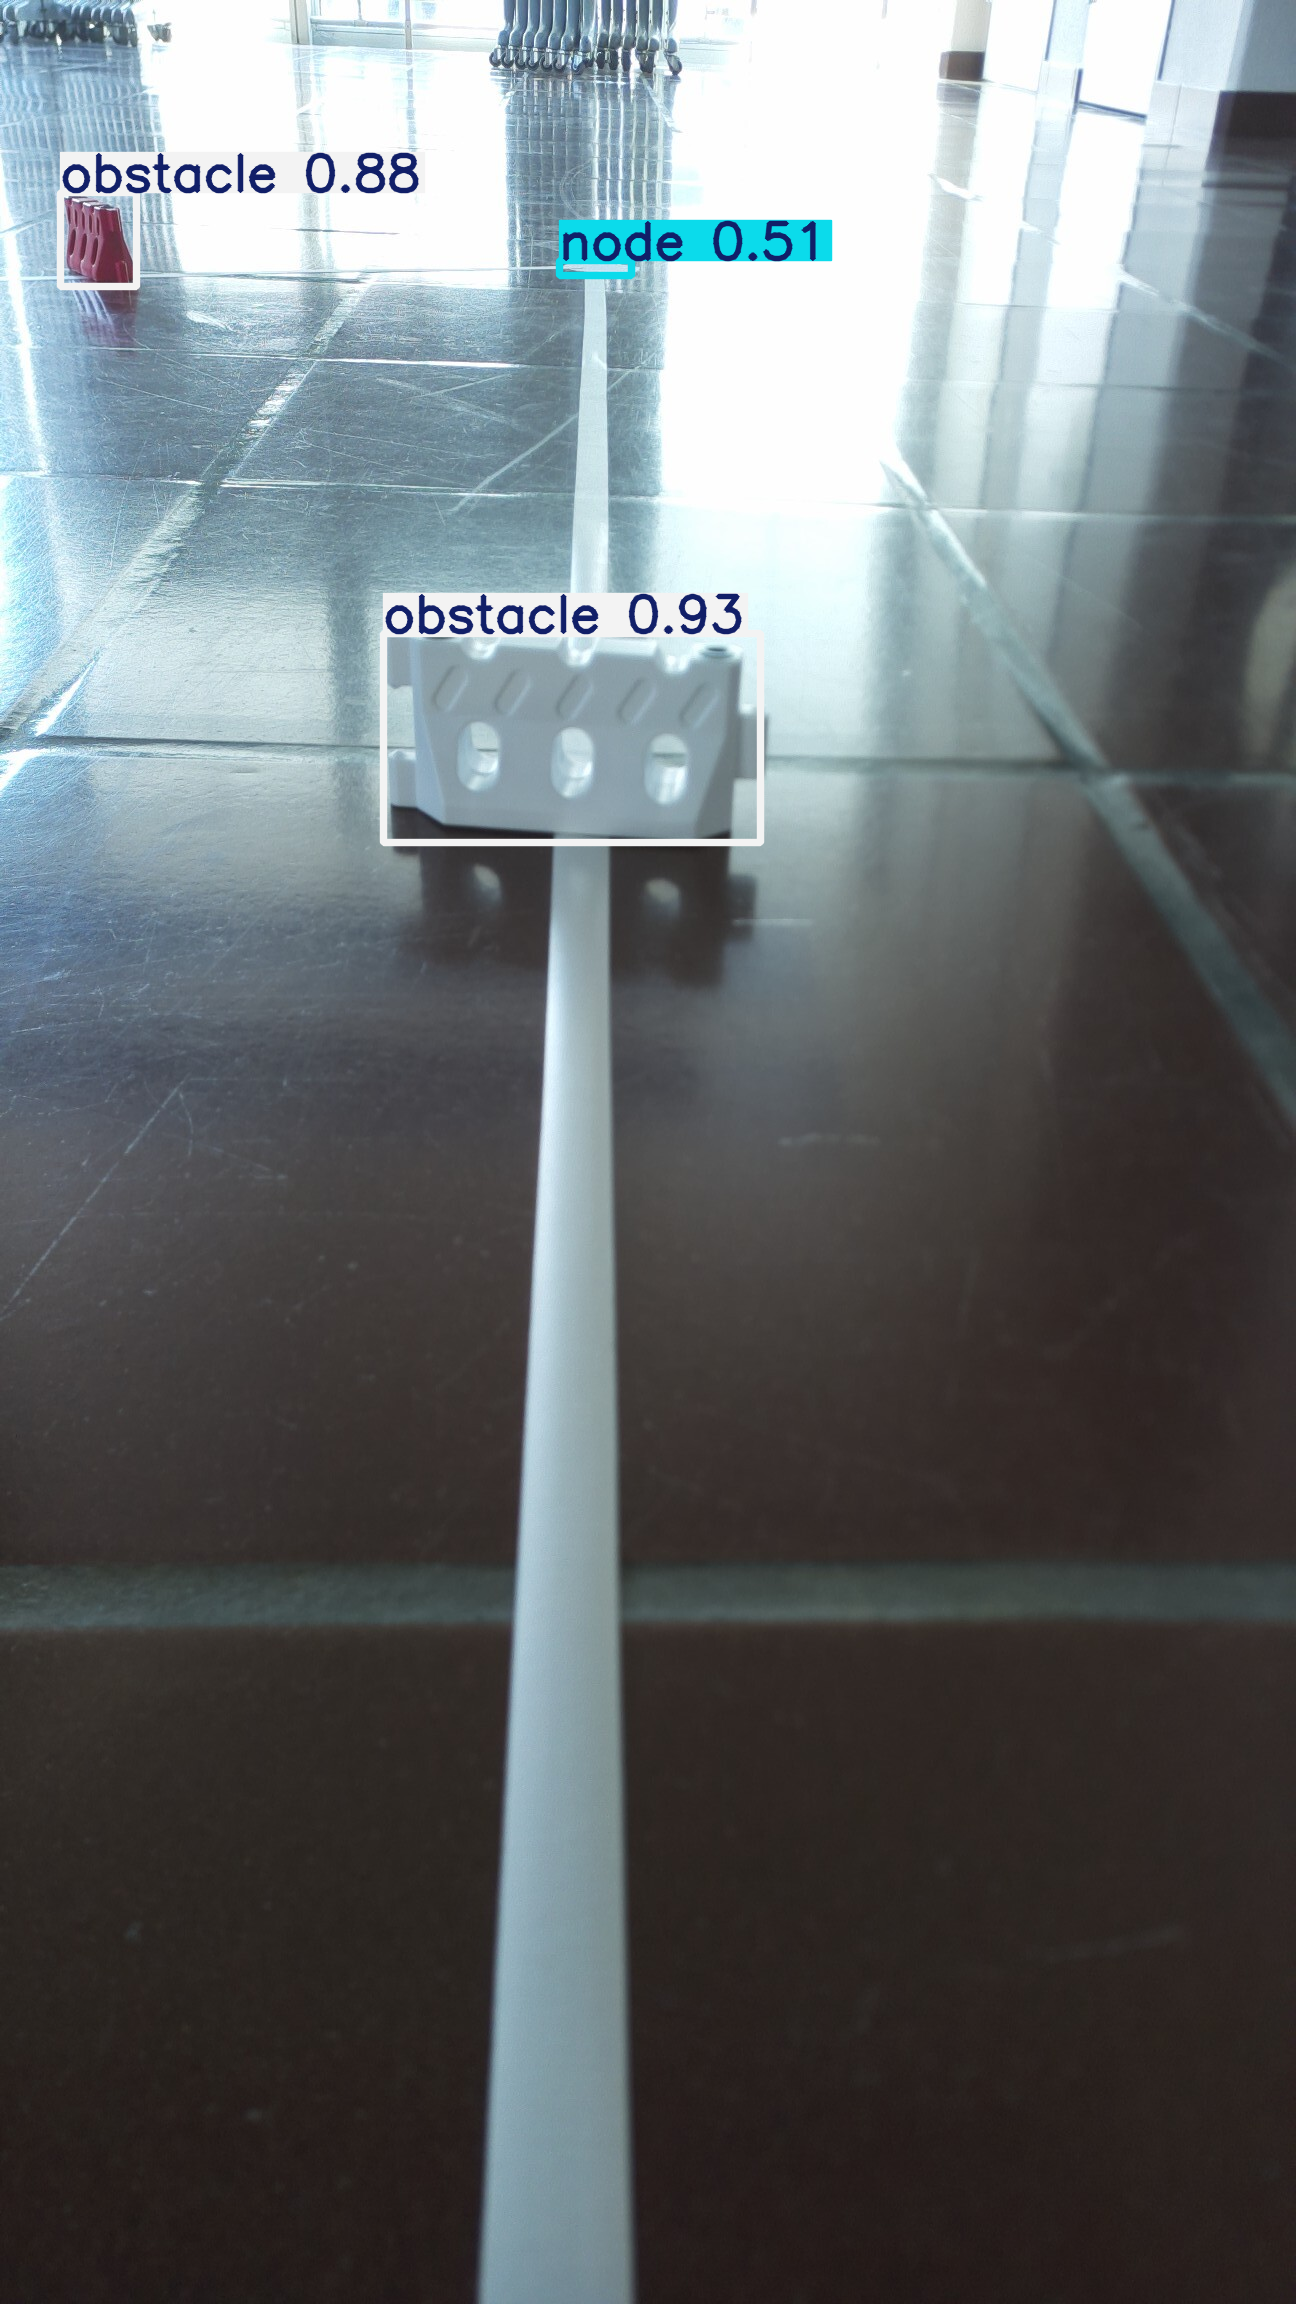
\includegraphics[width=\linewidth]{assets/IT/testing/yolo/2_barriers_1_node_annot.png}
\end{minipage}        
        &Barriere erkannt.&Barriere erkannt.&Erfüllt \\
        \hline
        6&
\begin{minipage}{.18\textwidth}
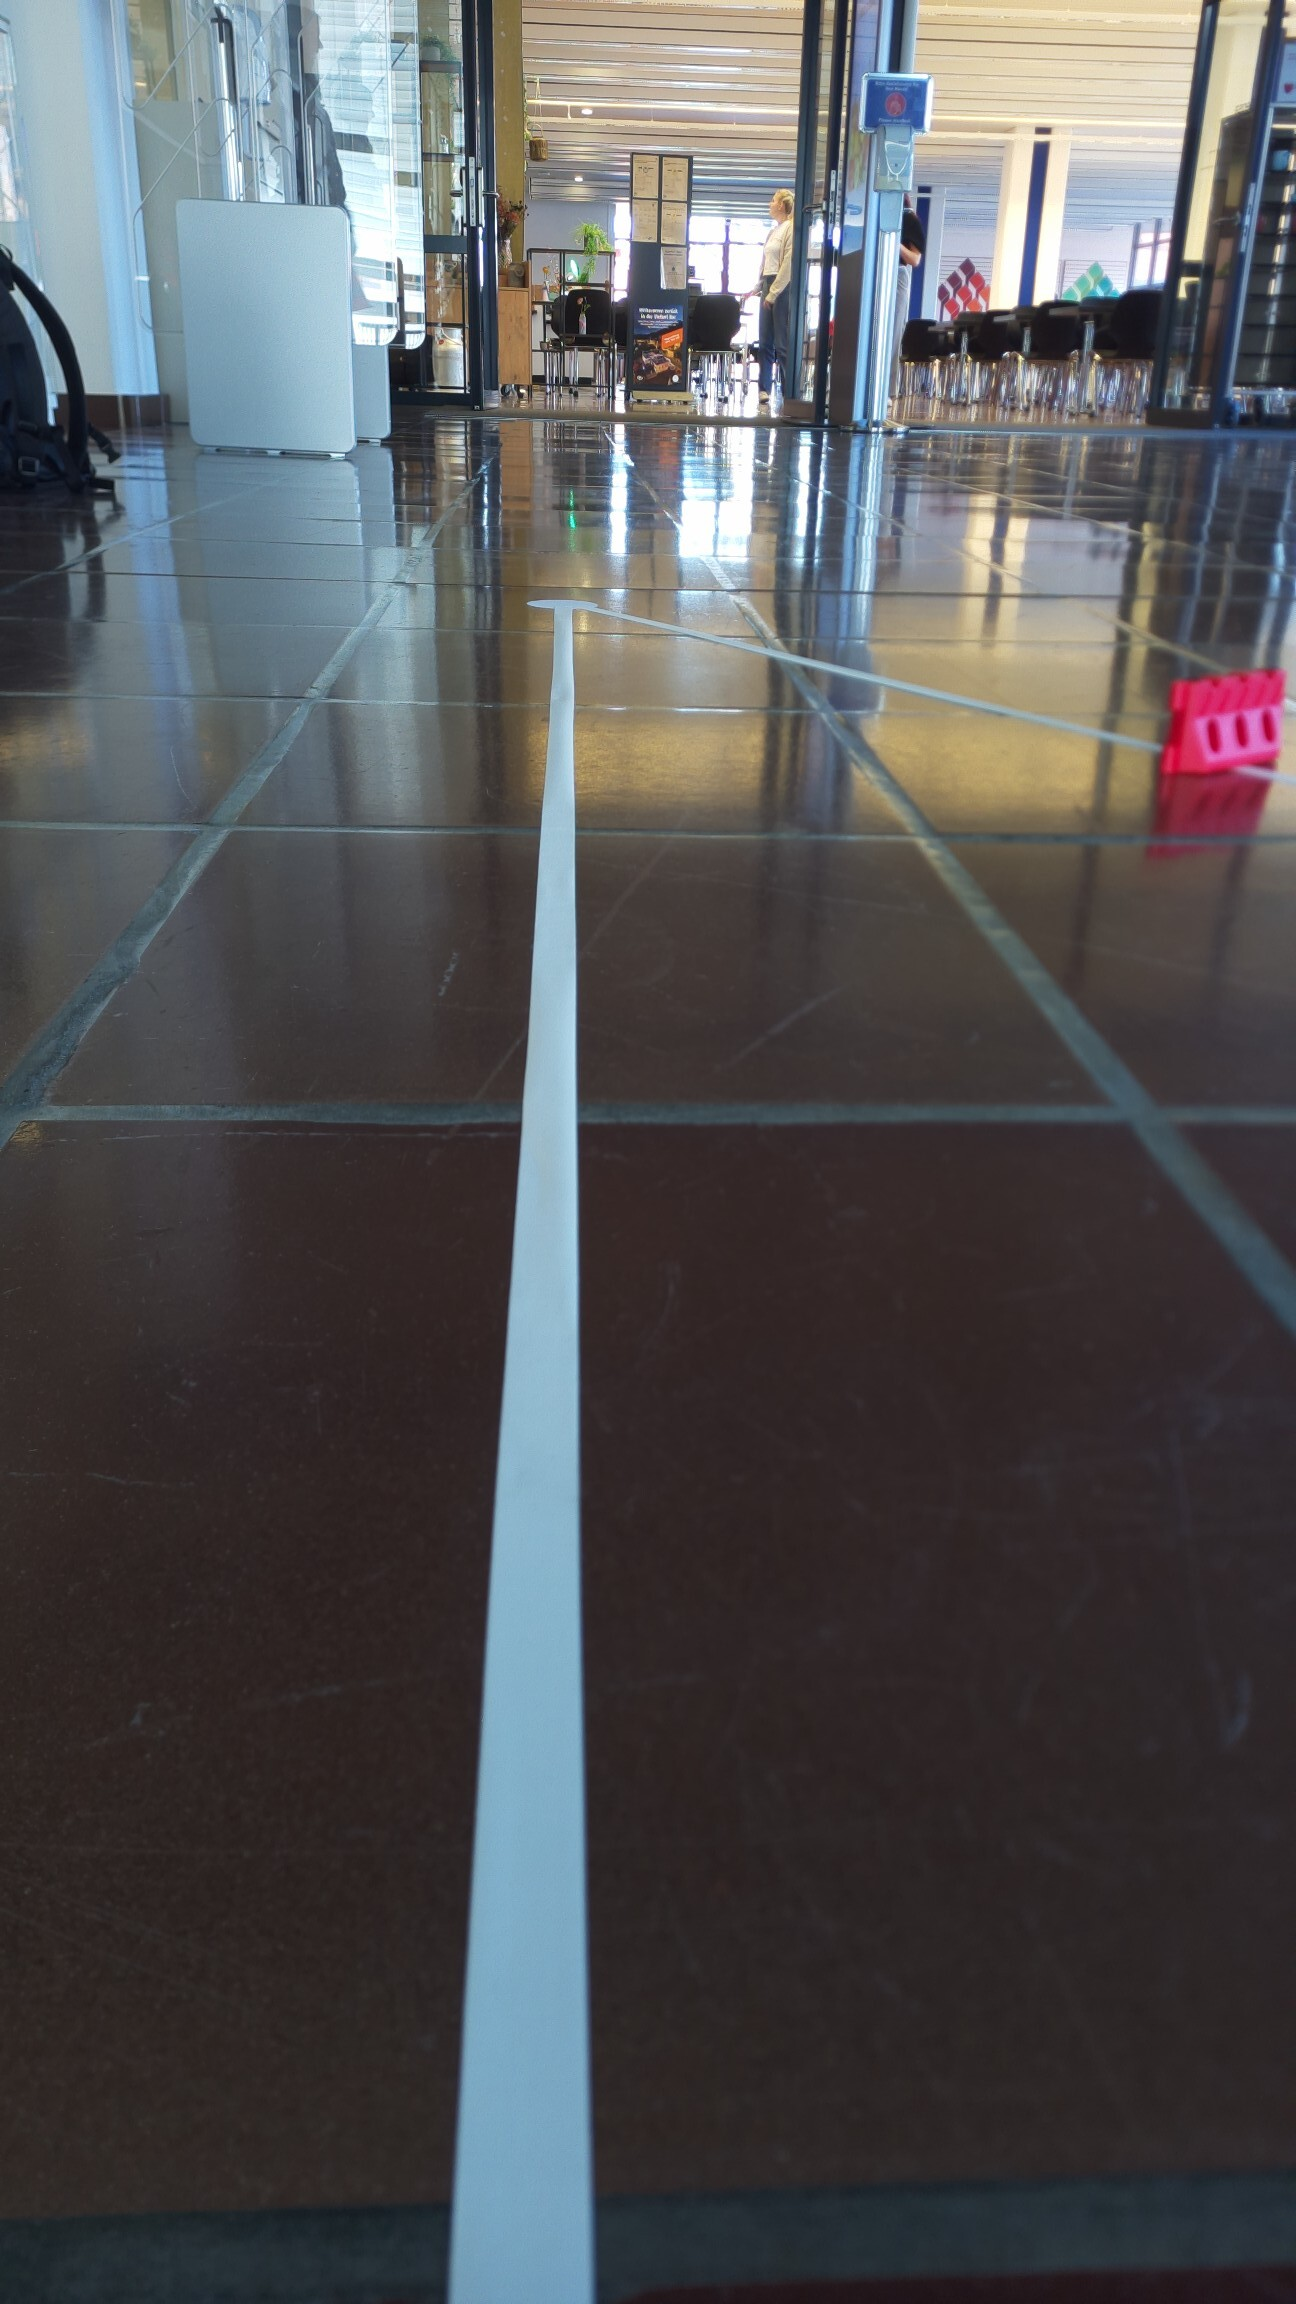
\includegraphics[width=\linewidth]{assets/IT/testing/yolo/node-obst-on-the-side.jpg}
\end{minipage}
        &
\begin{minipage}{.18\textwidth}
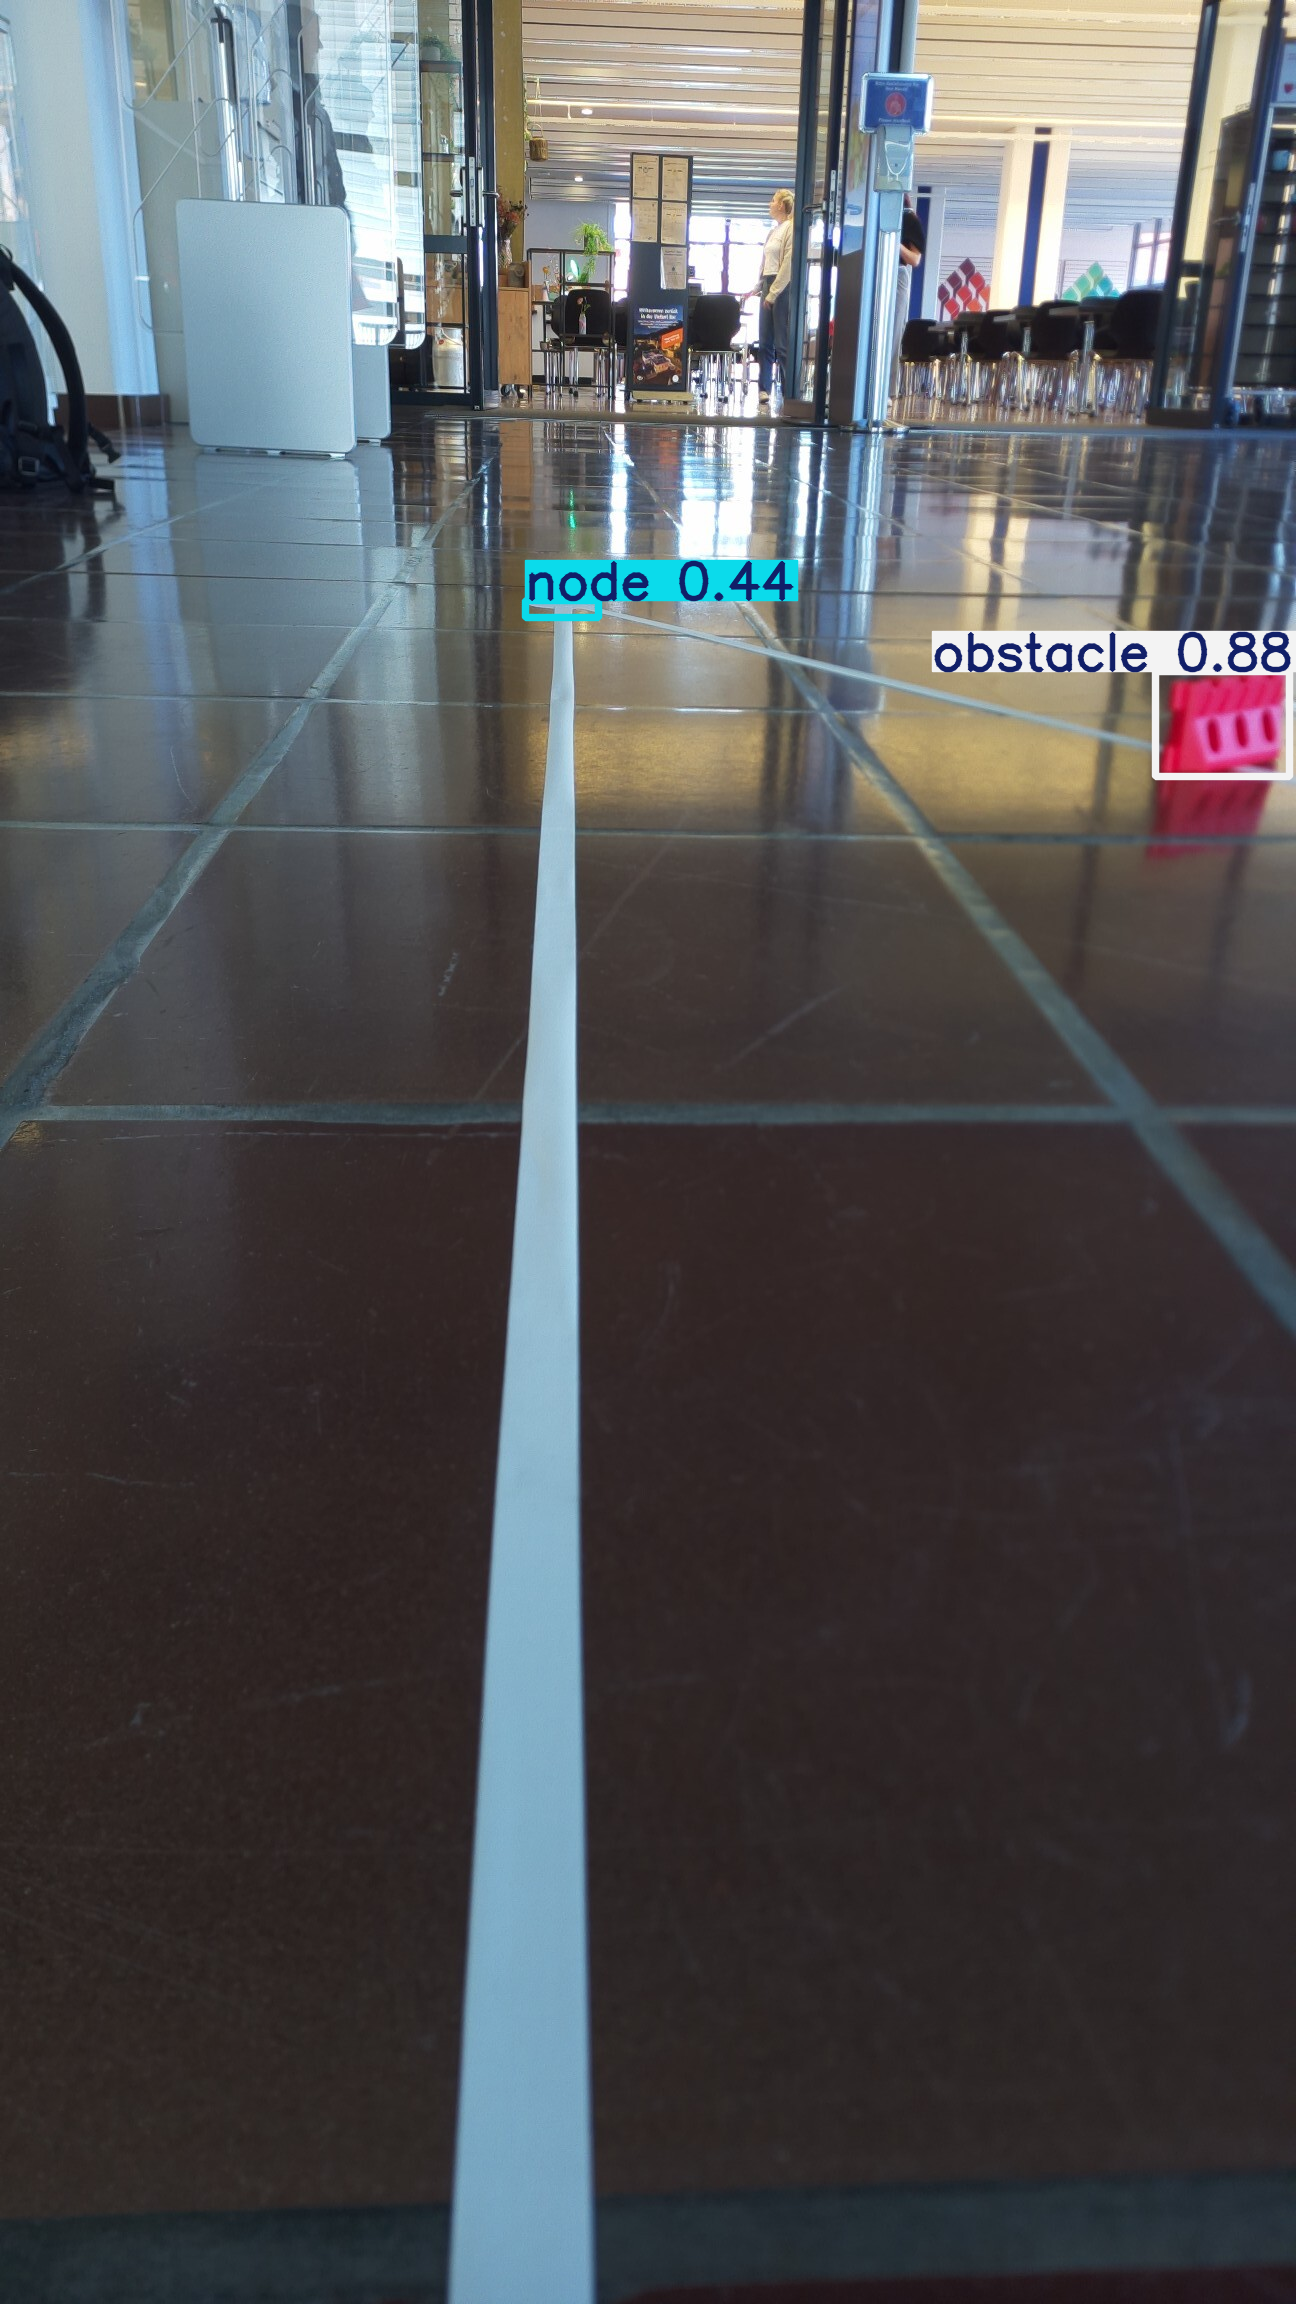
\includegraphics[width=\linewidth]{assets/IT/testing/yolo/node-obst-on-the-side_annot.png}
\end{minipage}
        &Knoten erkannt.&Knoten erkannt.& Erfüllt\\
  \hline


\end{tabularx}
\caption{Object Detector Testprotokoll}
\label{table:object-det-test}
\end{table}

Auf dem folgenden Bild \ref{img:object_detector_unittests} sind alle Unittests ersichtlich, die alle erfolgreich waren.

\begin{figure}[H]
\centering
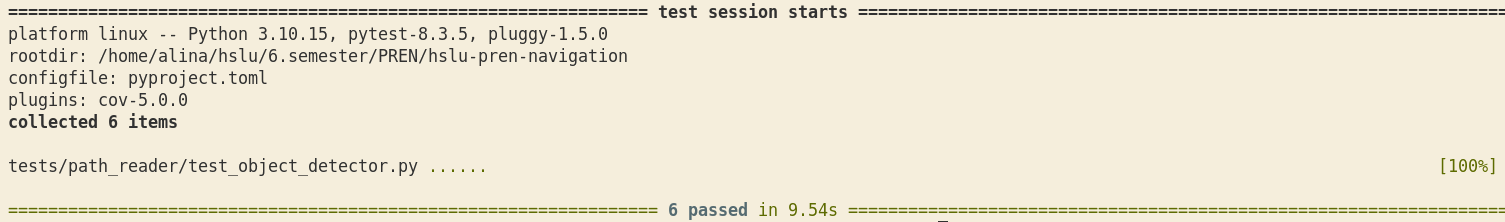
\includegraphics[width=\textwidth]{assets/IT/testing/yolo/object-detector-unittests.png}
\caption{Alle Object Detector Unittests}
\label{img:object_detector_unittests}
\end{figure}





%%%%%%%%%%%%%%%%%%%%%%% protocol opencv calibration %%%%%%%%%%%%%%%%%%%%%%%%

\addcontentsline{toc}
{subsection}
{Protokoll OpenCV Kalibration}
\label{opencv}

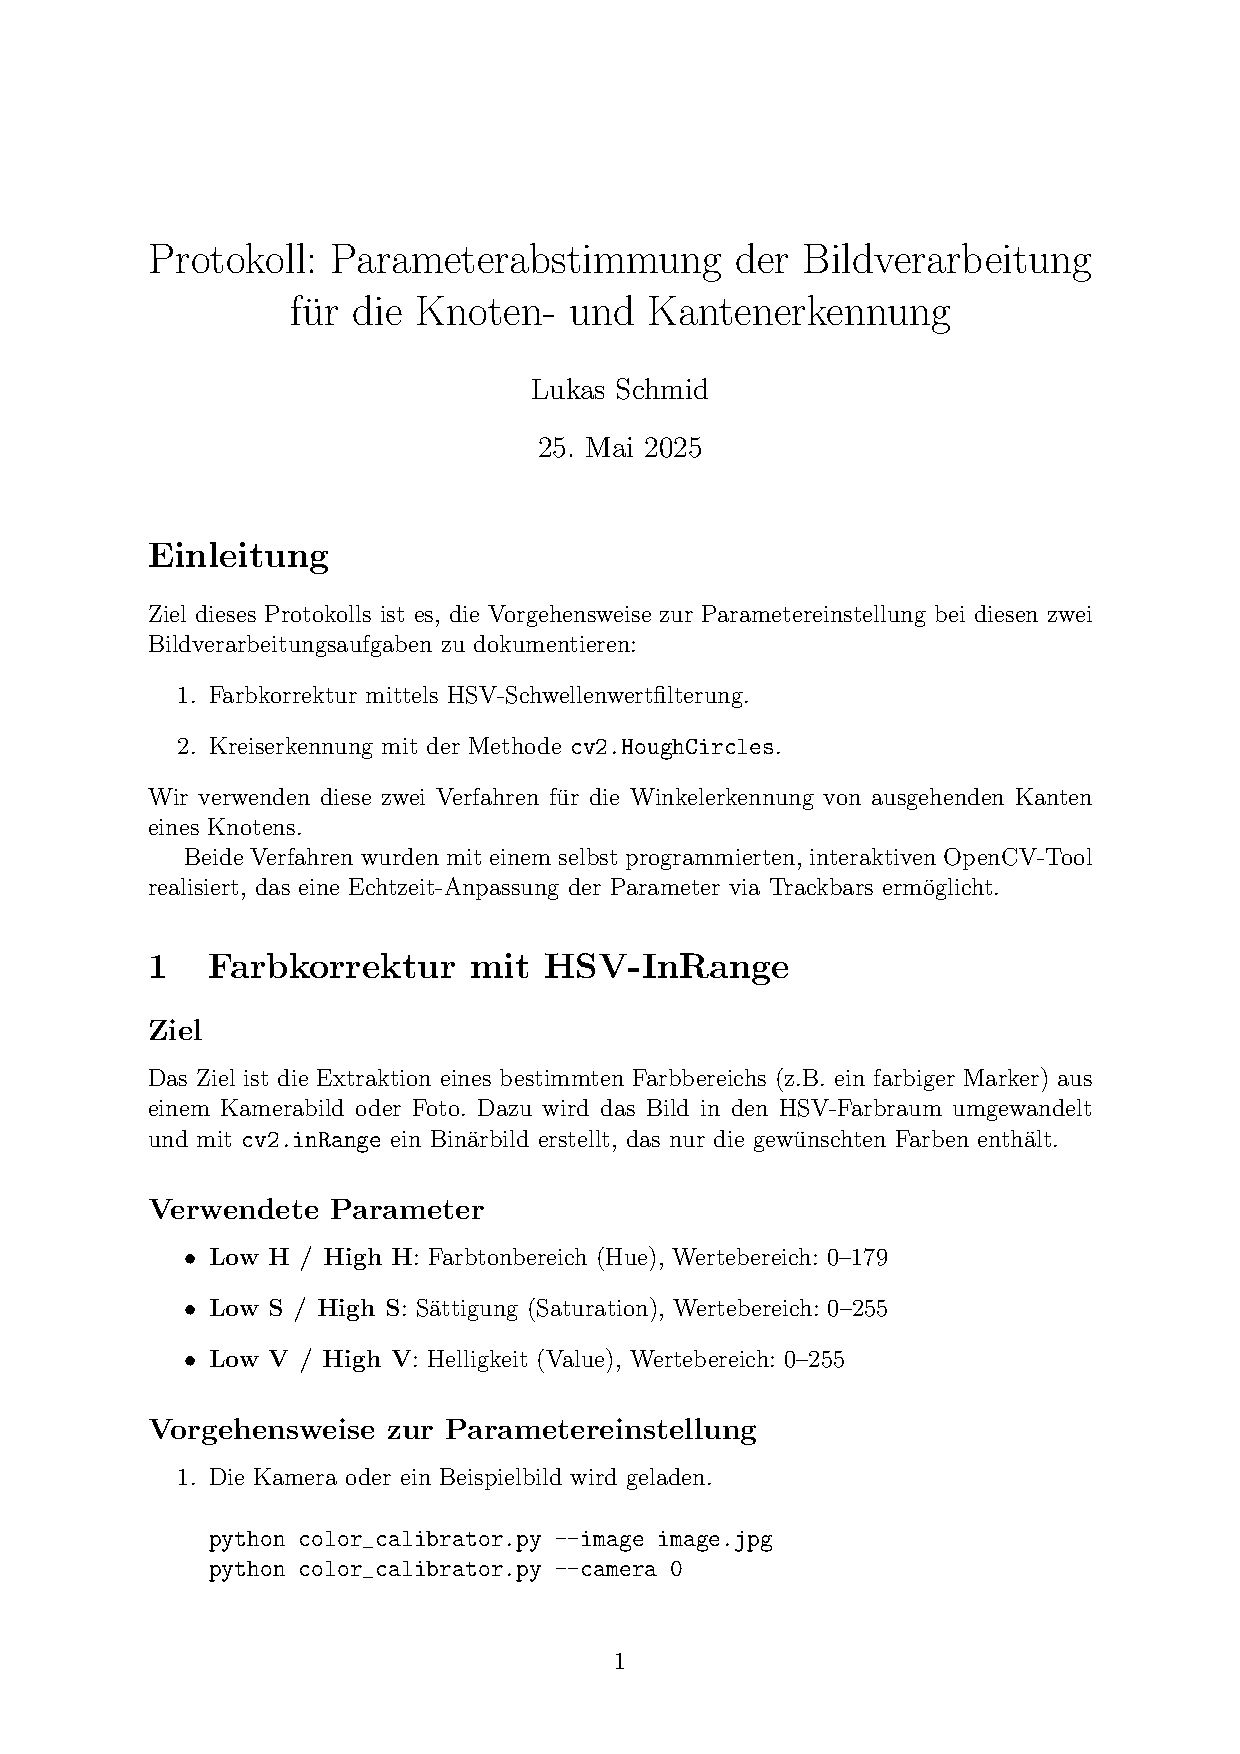
\includepdf[pages=-]{assets/IT/testing/protocol_opencv_calibration.pdf}


%%%%%%%%%%%%%%%%%%%%%%% testprocotol static node and edge detection %%%%%%%%%%%%%%%%%%%%%%%%

\addcontentsline{toc}
{subsection}
{Testprotokoll Ausgehende Kanten erkennen}
\label{outgoing-lines-test}

\includepdf[pages=-]{assets/IT/testing/testprotocol_static_node_edge_detection.pdf}


%%%%%%%%%%%%%%%%%%%%%%% testprocotol static node and edge detection %%%%%%%%%%%%%%%%%%%%%%%%

\addcontentsline{toc}
{subsection}
{Testprotokoll Statische Traversierung}
\label{statische-traver}

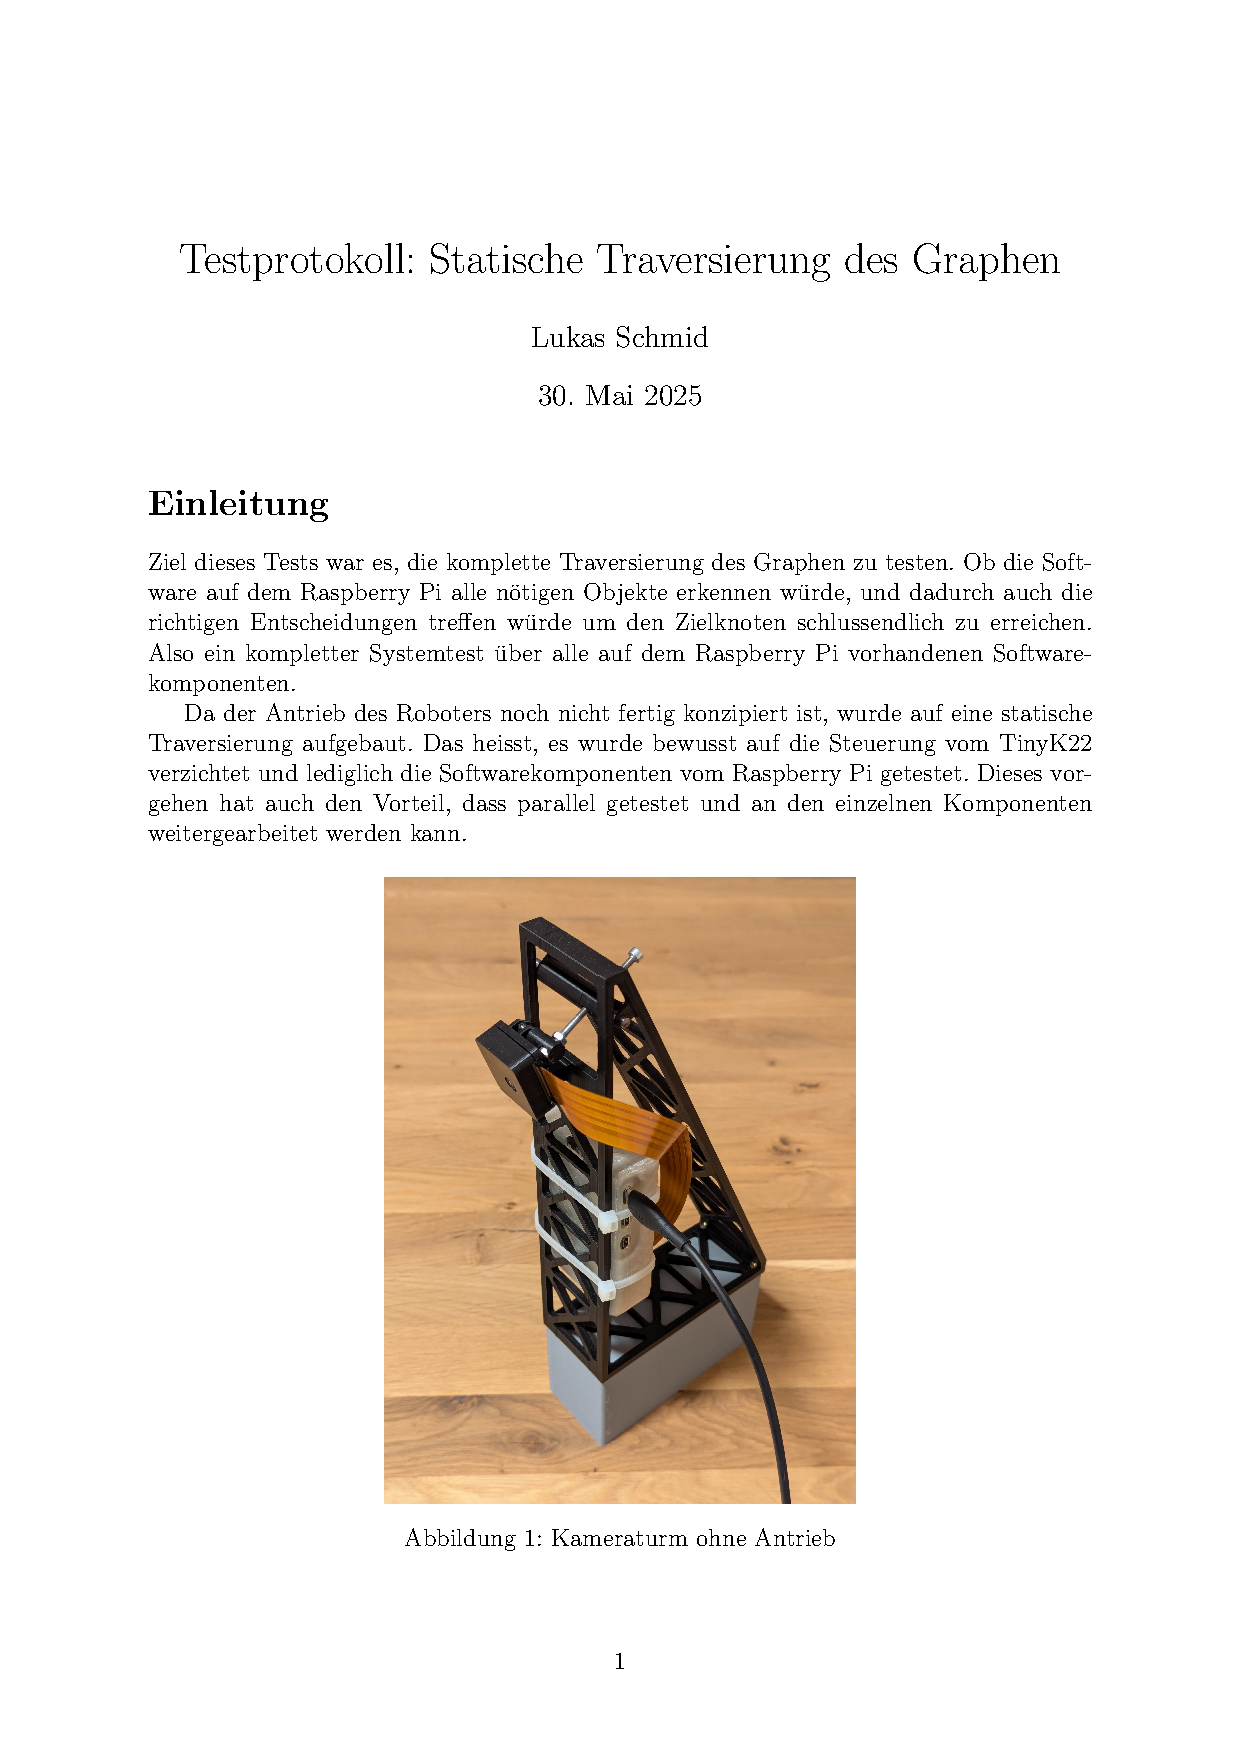
\includepdf[pages=-]{assets/IT/testing/testprotocol_static_traversal.pdf}

% \clearpage
% \phantomsection
% \addcontentsline{toc}{subsection}{Testprotokoll Statische Traversierung}
% \section*{Testprotokoll Statische Traversierung}
% \label{statische-traver}

% 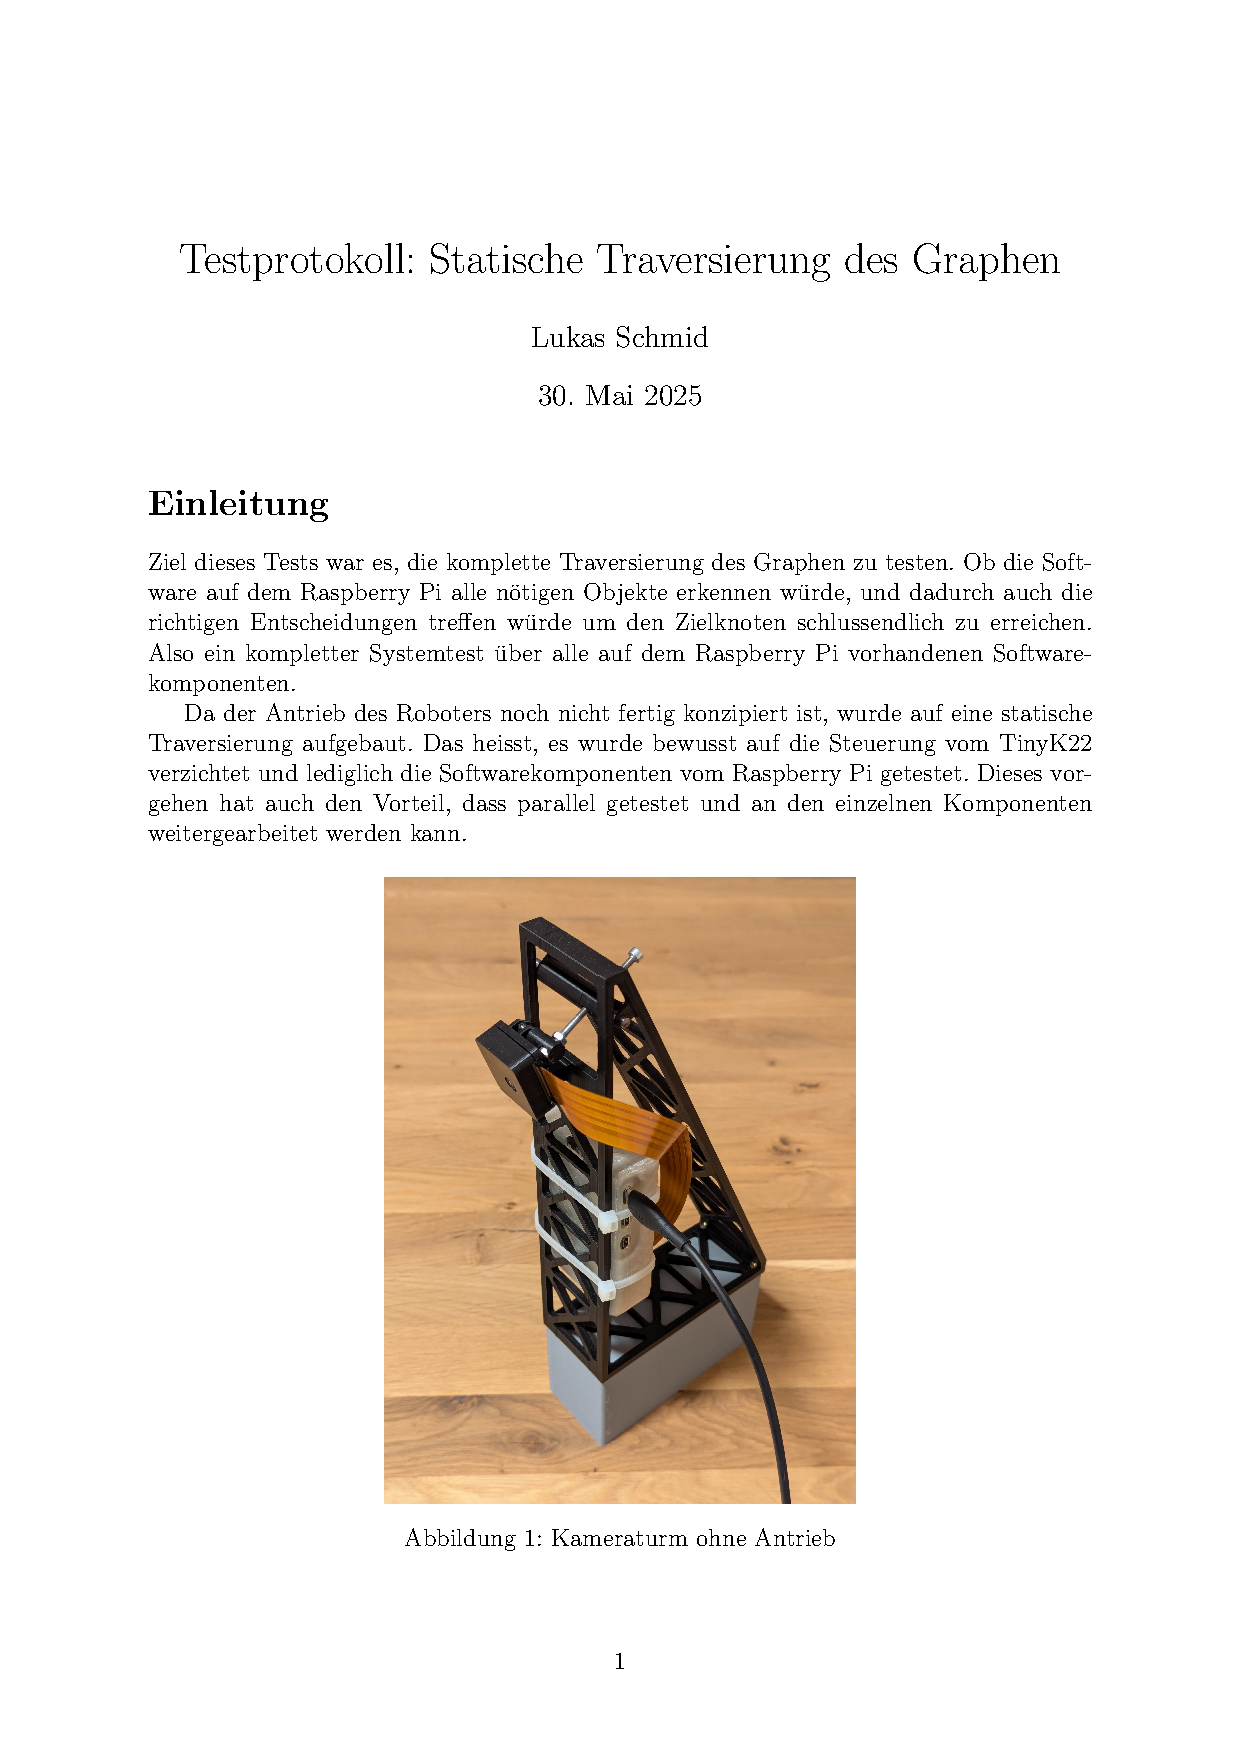
\includepdf[pages=-]{assets/IT/testing/testprotocol_static_traversal.pdf}


%%%%%%%%%%%%%%%%%%%%%%% testprocotol Fahrregelung mit Liniensensoren %%%%%%%%%%%%%%%%%%%%%%%%

\addcontentsline{toc}
{subsection}
{Testprotokoll Liniensensor}

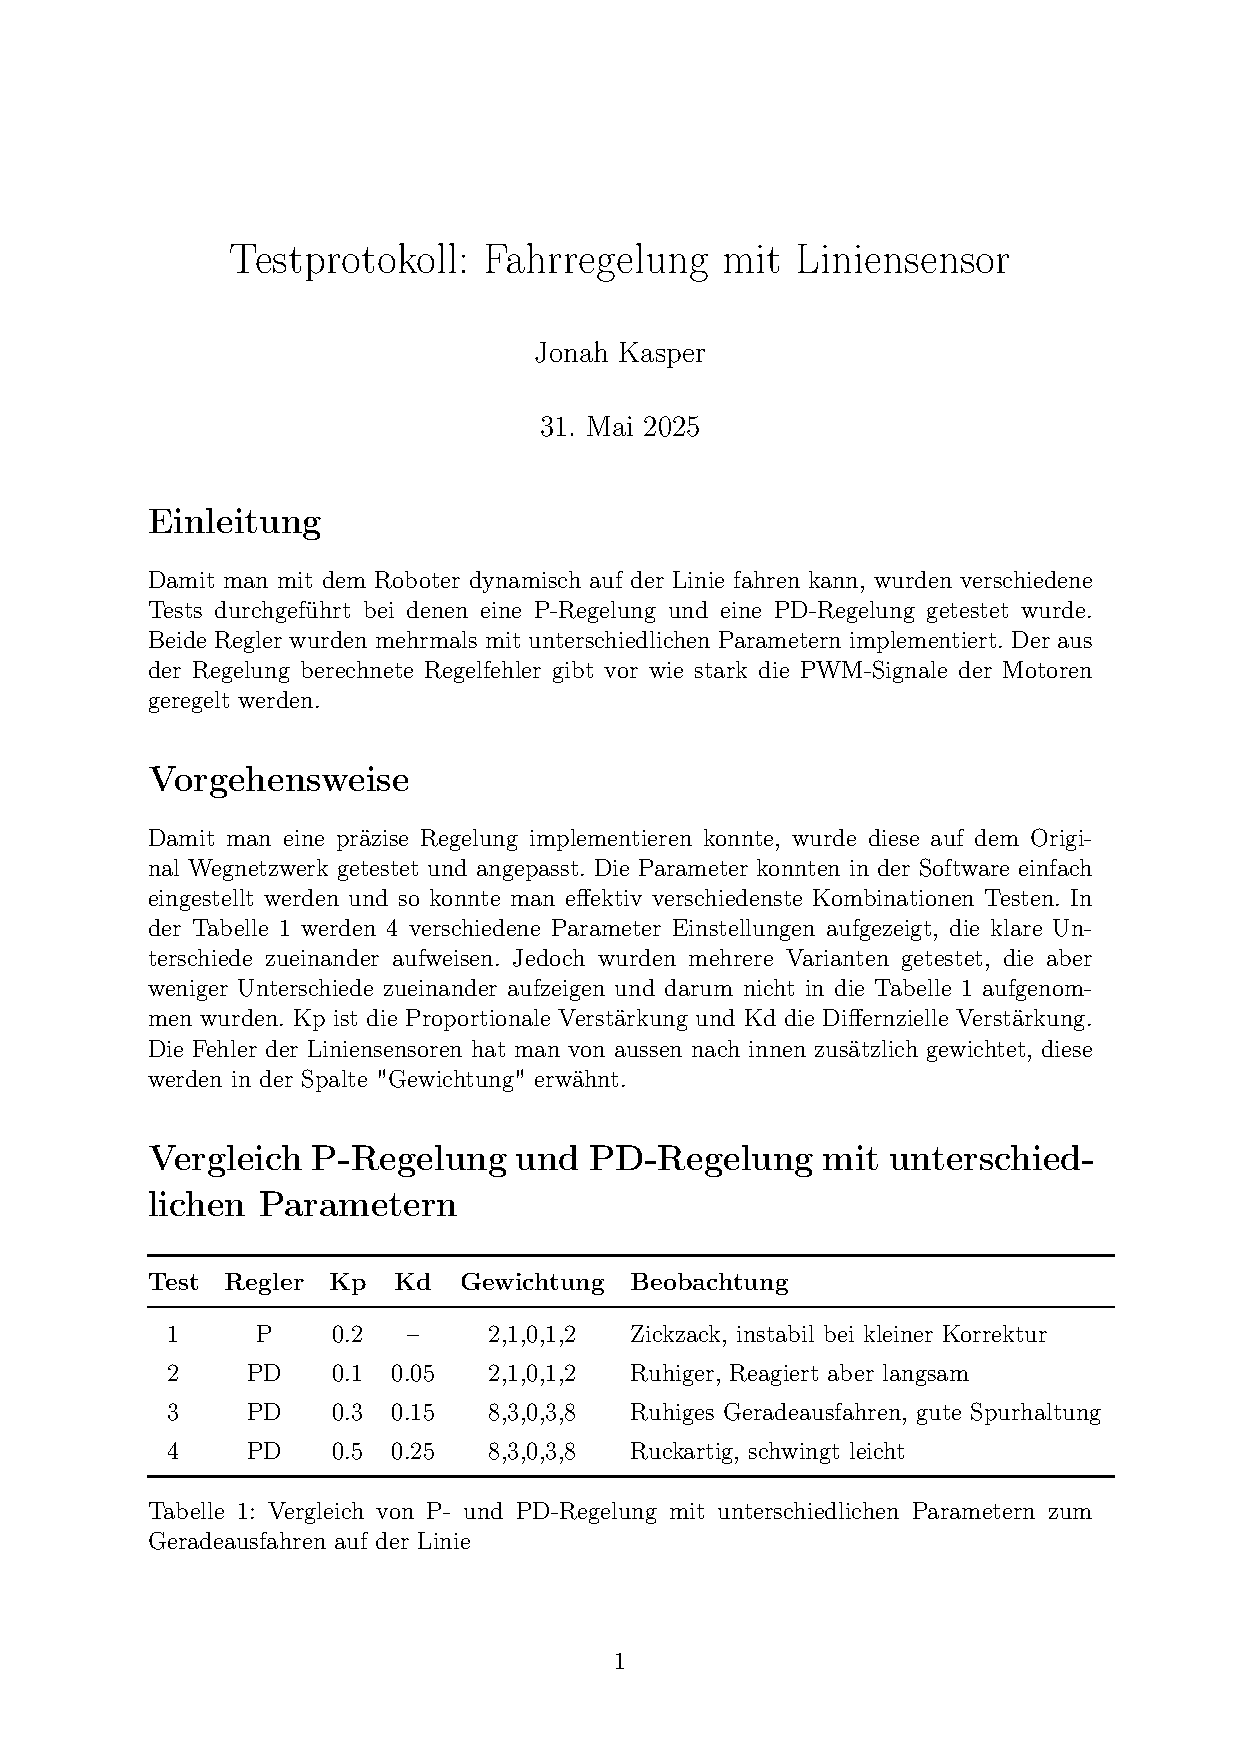
\includepdf[pages=-]{assets/ET/Testprotokolle/Testprotokoll_Regelung.pdf}



%%%%%%%%%%%%%%%%%%%%%%%5 drehen mit encoder %%%%%%%%%%%%%%%%%%%%%%%%5

\newpage
\subsection*{Untersuchung Drehen mit Encodern}\label{drehen-encoder}
  \addcontentsline{toc}
    {subsection}
    {Untersuchung Drehen mit Encodern}

Es gab Probleme mit dem Drehen. Der Winkel, der gedreht werden sollte, wurde sehr ungenau umgesetzt und es konnte kein Regelmässigkeit darin erkannt werden.

Die Hardware, sowie der zugehörige Code wurde auf Fehler überprüft. Mit dem Oszilloskop wurden die vom Encoder erzeugten Signale analysiert. Dabei zeigte sich ein hochfrequentes Rauschen, dessen Amplituden jedoch zu gering sind, um nennenswerte Fehler zu verursachen. Die Ursache des Rauschens konnte auf die verwendeten DC-Motoren zurückgeführt werden.

Anschliessend wurde ein Encoder mithilfe eines Frequenzgenerators simuliert, um das Zähleverhalten des implementierten Codes zu überprüfen. Die Taktfrequenz wurde auf 500 Hz eingestellt. Kanal 2 wurde mit einer Phasenverschiebung von 90\textdegree \ nacheilend konfiguriert. Unter diesen Bedingungen sollte der implementierte Zähler eine Inkrementierung vornehmen.

Das Taktsignal wurde für eine Dauer von 2 Sekunden angelegt, was direkt am Frequenzgenerator eingestellt wurde. Der erwartete Endwert des Zählers lag entsprechend bei etwa 1000.

\begin{table}[H]
\centering
\caption{Ergebnisse der aufgezeichneten Taktimpulse Decoder}
\label{tab:taktergebnisse_de}
\begin{tabular}{|c|c|}
\hline
\textbf{Messung} & \textbf{Aufgezeichnete Takte} \\
\hline
1 & 723 \\
2 & 1397 \\
3 & 1412 \\
4 & 655 \\
\hline
\end{tabular}
\end{table}

Wie aus Tabelle \ref{tab:taktergebnisse_de} ersichtlich ist, weichen die aufgezeichneten Werte um bis zu 41\% vom erwarteten Sollwert ab. Diese Abweichung ist zu gross, um eine präzise Regelung darauf aufzubauen.

Es wurde ebenfalls der Code des MCCAR untersucht. Der Code liest die Encoder auf eine andere Weise aus. Anstelle der integrierten Decoder, wurde ein eigener Decoder implementiert. Dazu wird das Input Capture verwendet. Dies hat den Vorteil, dass die Geschwindigkeit der einzelnen Räder berechnet werden kann.

\begin{table}[H]
\centering
\caption{Ergebnisse der aufgezeichneten Taktimpulse Input Capture}
\label{tab:taktergebnisse_im}
\begin{tabular}{|c|c|}
\hline
\textbf{Messung} & \textbf{Aufgezeichnete Takte} \\
\hline
1 & 902 \\
2 & 1252 \\
3 & 842 \\
4 & 876 \\
\hline
\end{tabular}
\end{table}

Die Abweichung beim Input Capture ist geringer als bei den integrierten Decodern, liegt jedoch immer noch bei etwa 25\% (siehe Tabelle \ref{tab:taktergebnisse_im}). Dies ist zu viel. Die Encoder können nicht verwendet werden um sich genau zu drehen.


%%%%%%%%%%%%%%%%%%%%%%%%%%%%%%%%%%%%%%%%%% drehehn gyro %%%%%%%%%%%%%%%5

\newpage
\subsection*{Tests mit Gyroskop}\label{drehen-gyro}
  \addcontentsline{toc}
    {subsection}
    {Tests mit Gyroskop}

Die ersten Tests mit dem Gryskop wurden mit einem Bread Board durchgeführt und wurde mit einem Tiny K22 verbunden. Auf diese Weise kann das Gyroskop isoliert von den anderen Komponenten getestet werden. Damit das Gyroskop möglichst gerade sind konnte, wurde es aufgestellt. Durch die bereits angebrachten Widerstände konnte es nicht hingelegt werden. Das Setup ist ersichtlich auf Abbildung \ref{img:gyro-tests-1}.

\begin{figure}[H]
\centering
\includegraphics[width=10cm]{assets/ET/Gyroskop/gyro-breadboard.jpg}
\caption{Erste Gyroskop Tests}
\label{img:gyro-tests-1}
\end{figure}

Zuerst wurde ein simples Programm geschrieben, um die Werte über UART1 im Terminal auszulesen. Das Gyroskop gibt 16-Bit-Messwerte für jede Achse (X, Y und Z) im Big-Endian-Format aus, wobei das höchstwertige Byte zuerst übertragen wird. Da der Prozessor des TinyK22 im Little-Endian-Format arbeitet, müssen diese Bytes nach dem Empfang zuerst noch korrekt konvertiert werden.\footnote{https://wraycastle.com/de/blogs/knowledge-base/big-endian-little-endian}

Als nächstes wurde ein Programm geschrieben, das erwartet, dass das Gyroskop sich um einen bestimmten Winkel (in den folgenden Tests 90\textdegree) dreht und sobald der Winkel erreicht wird, wird eine Nachricht dafür ausgegeben. Dafür wurde das Breadboard in verschiedenen Geschwindigkeiten um 90\textdegree \ gedreht, bis die Nachricht erschien. Die Messung war in allen Geschwindigkeiten sehr genau. Der Wert war immer zwischen 90.0\textdegree \ und 90.5\textdegree.

Die folgenden Bewegungen wurden durchgeführt mit dem Gyroskop: 

\begin{figure}[H]
  \centering
  \begin{minipage}[b]{0.29\textwidth}
    \centering
    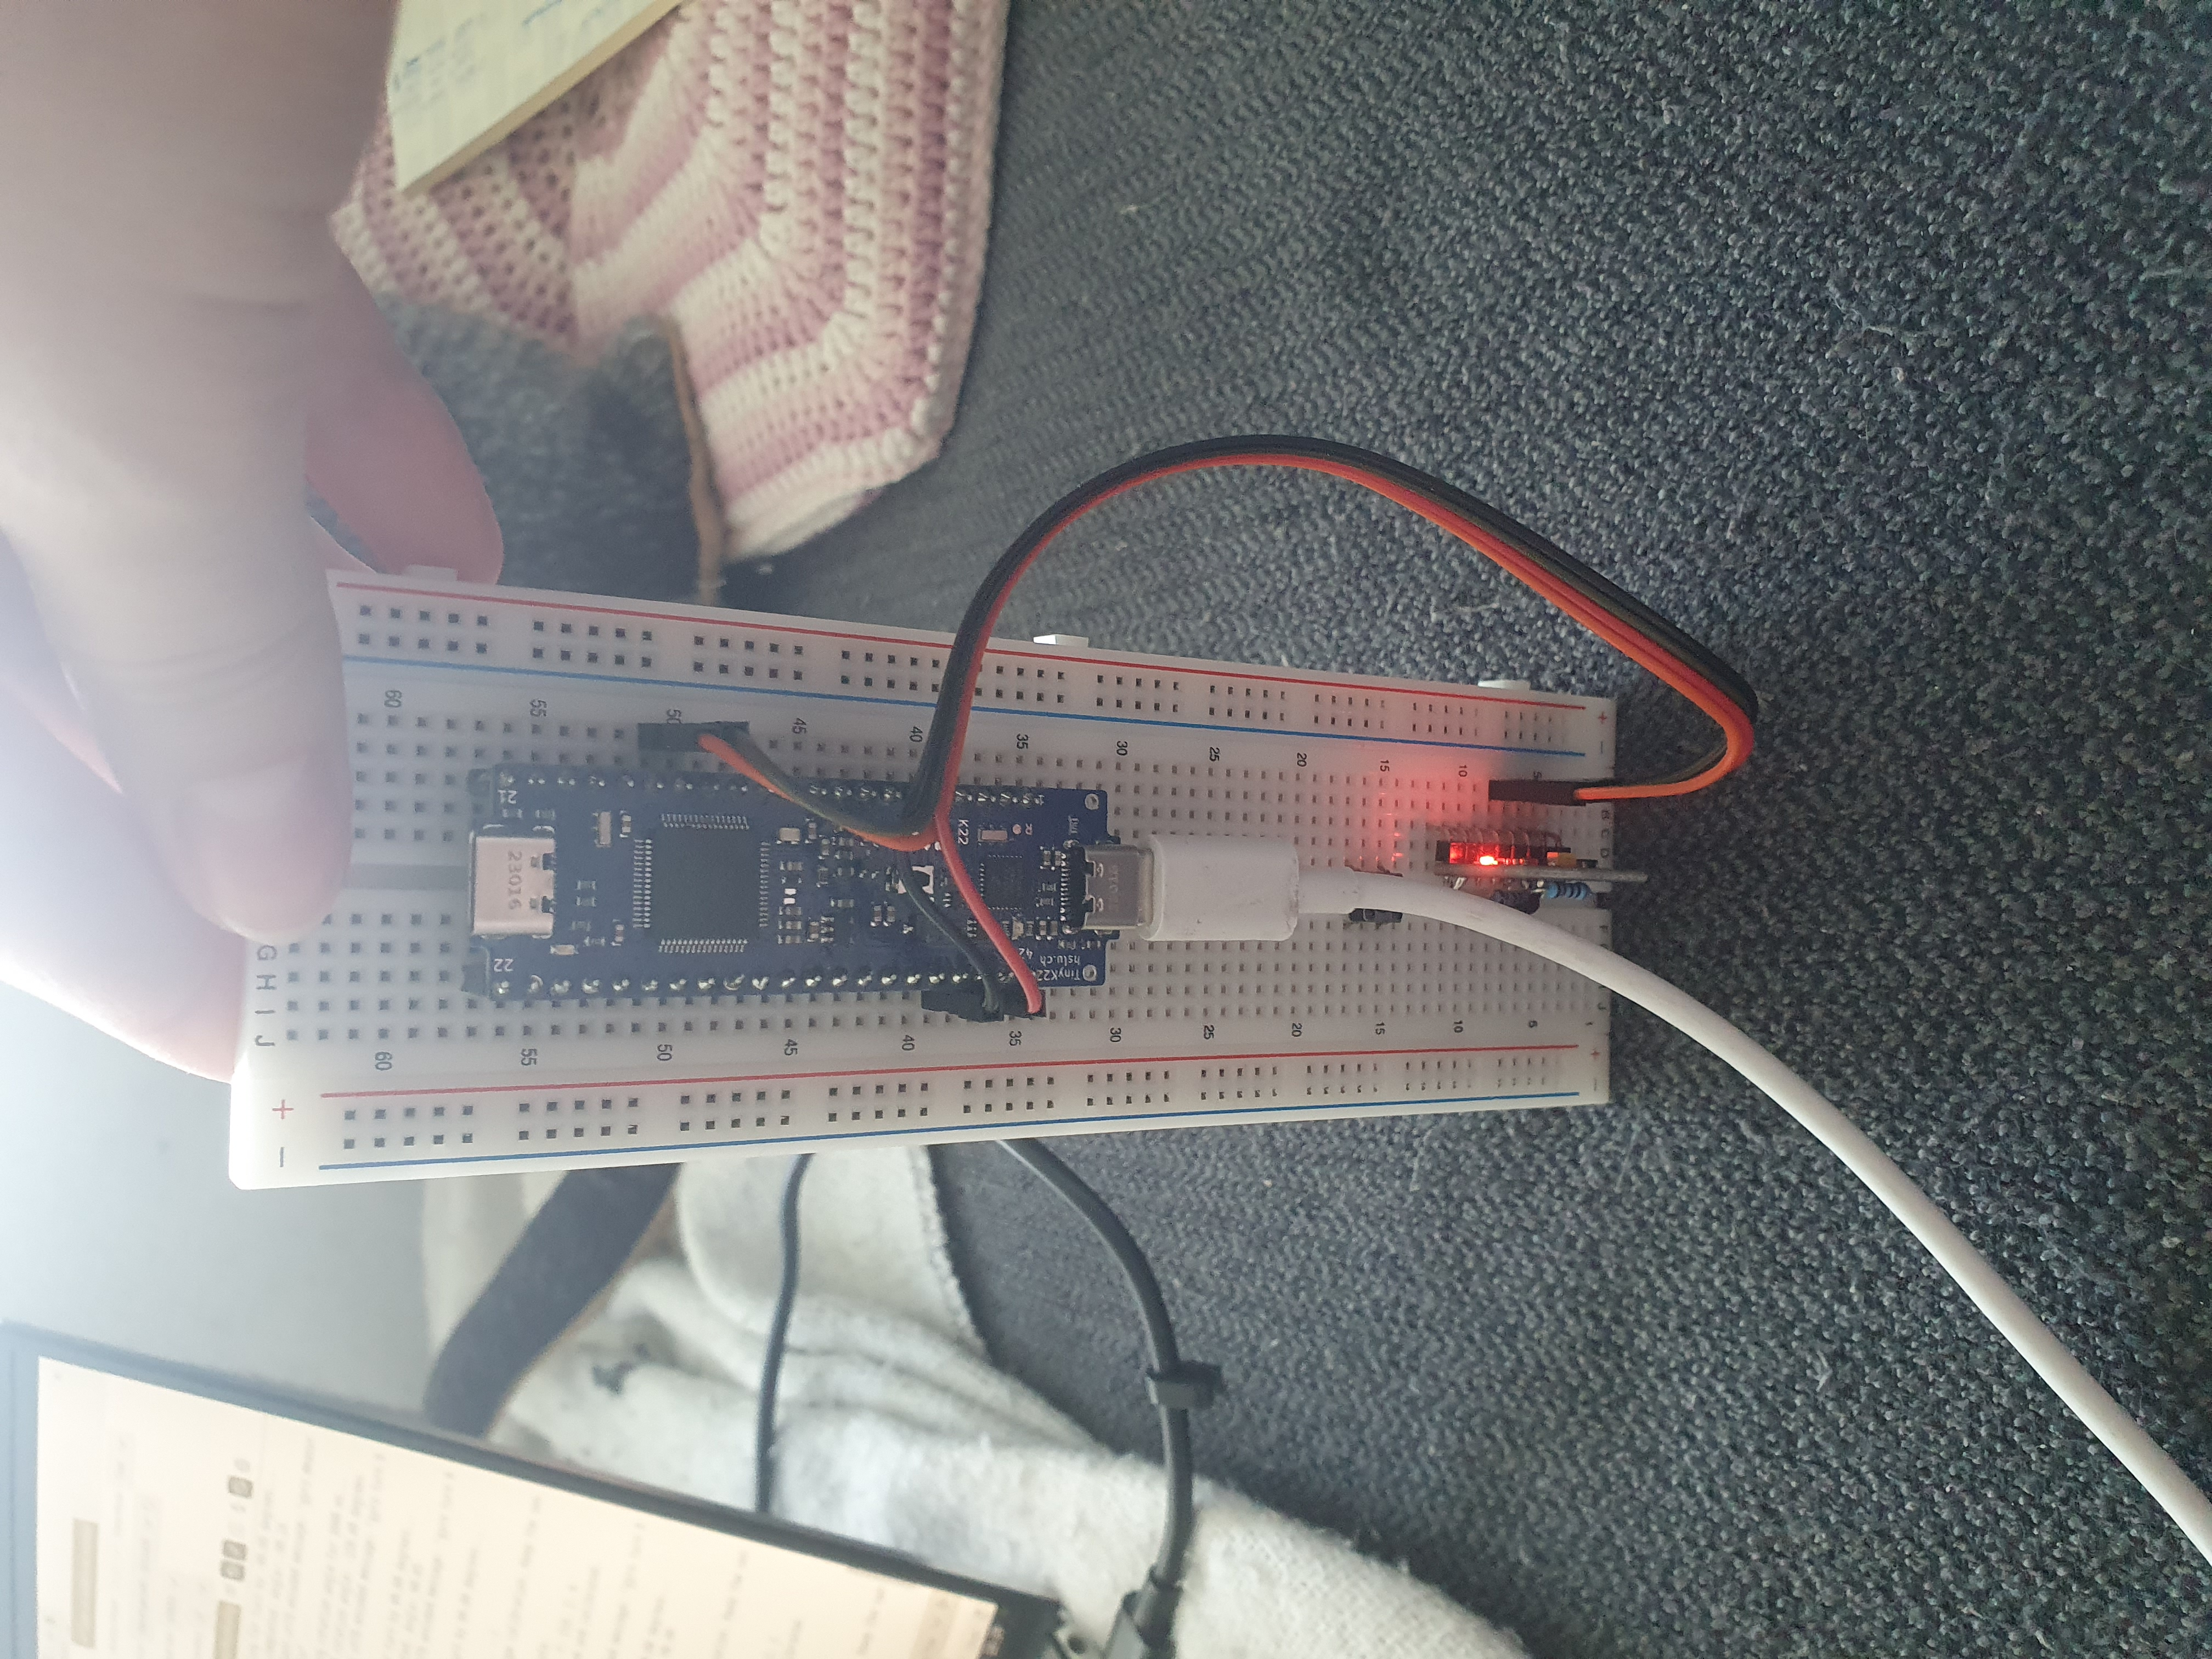
\includegraphics[width=\textwidth, angle=-90]{assets/ET/Gyroskop/gyro-0-deg.jpg}
    \caption{0 Grad}
    \label{fig:gyro-0}
  \end{minipage}
  \hfill
  \begin{minipage}[b]{0.29\textwidth}
    \centering
    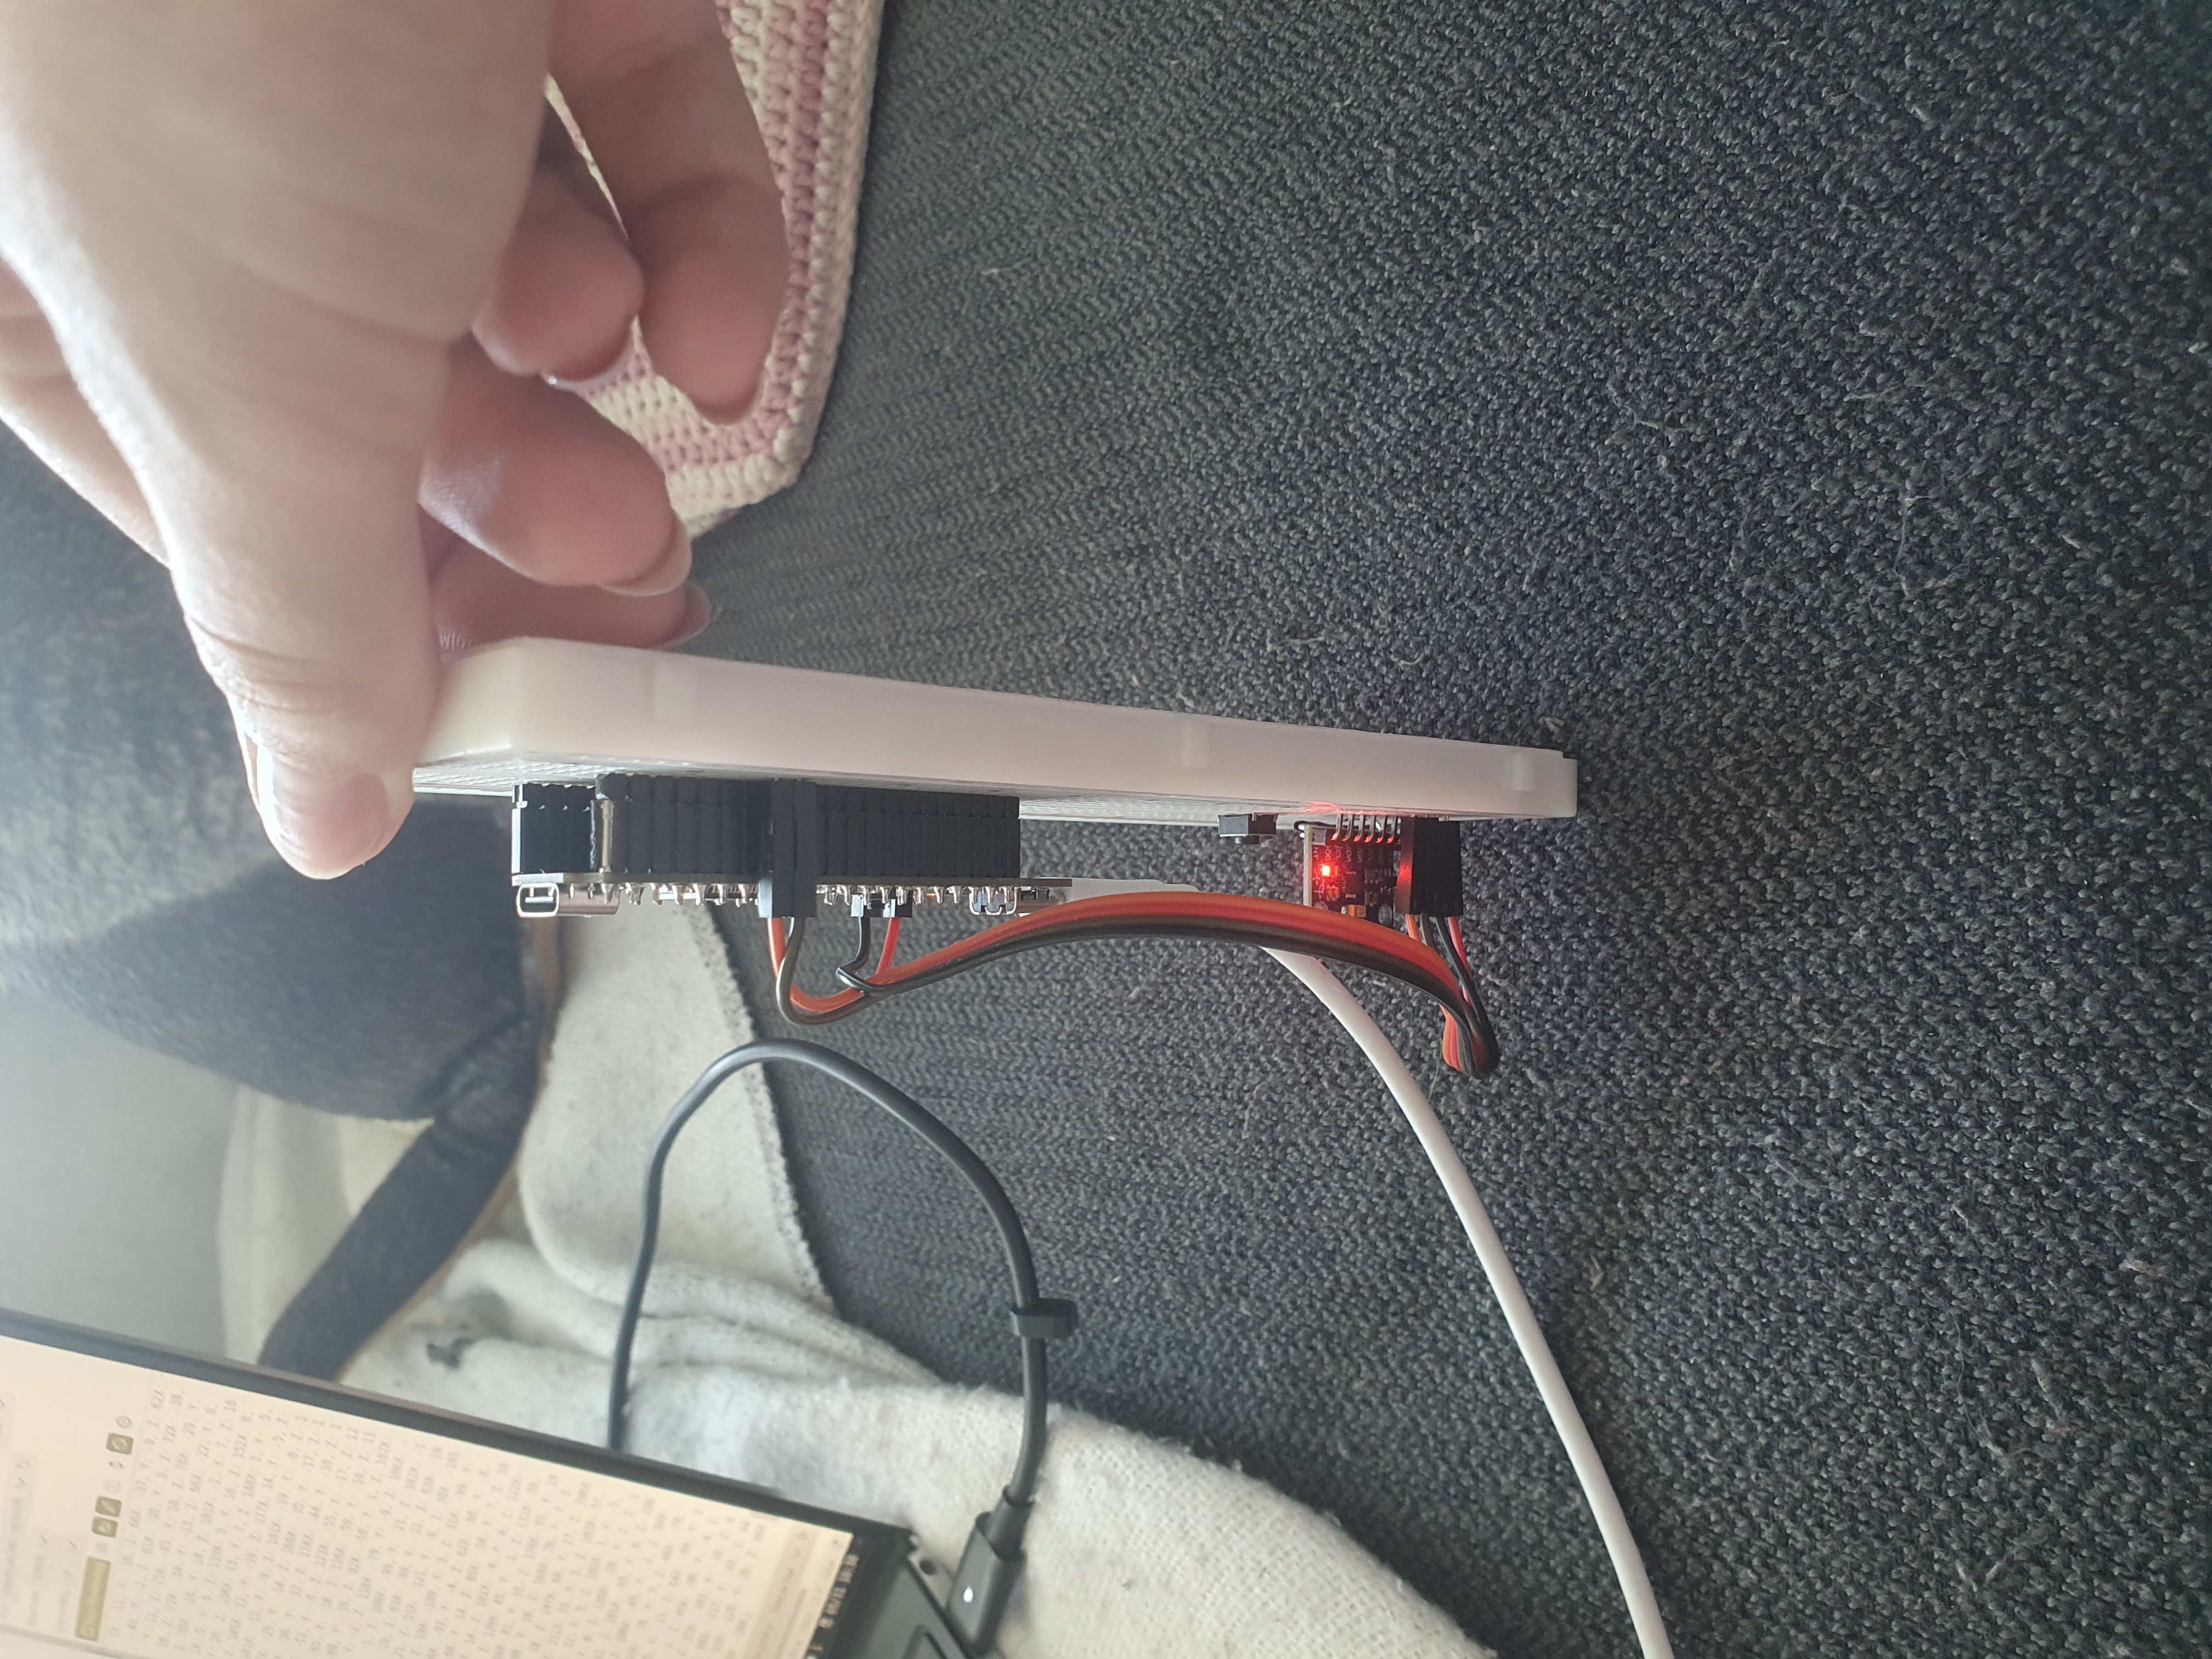
\includegraphics[width=\textwidth, angle=-90]{assets/ET/Gyroskop/gyro-90-deg.jpg}
    \caption{+90 Grad}
    \label{fig:gyro--90}
  \end{minipage}
    \hfill
  \begin{minipage}[b]{0.29\textwidth}
    \centering
    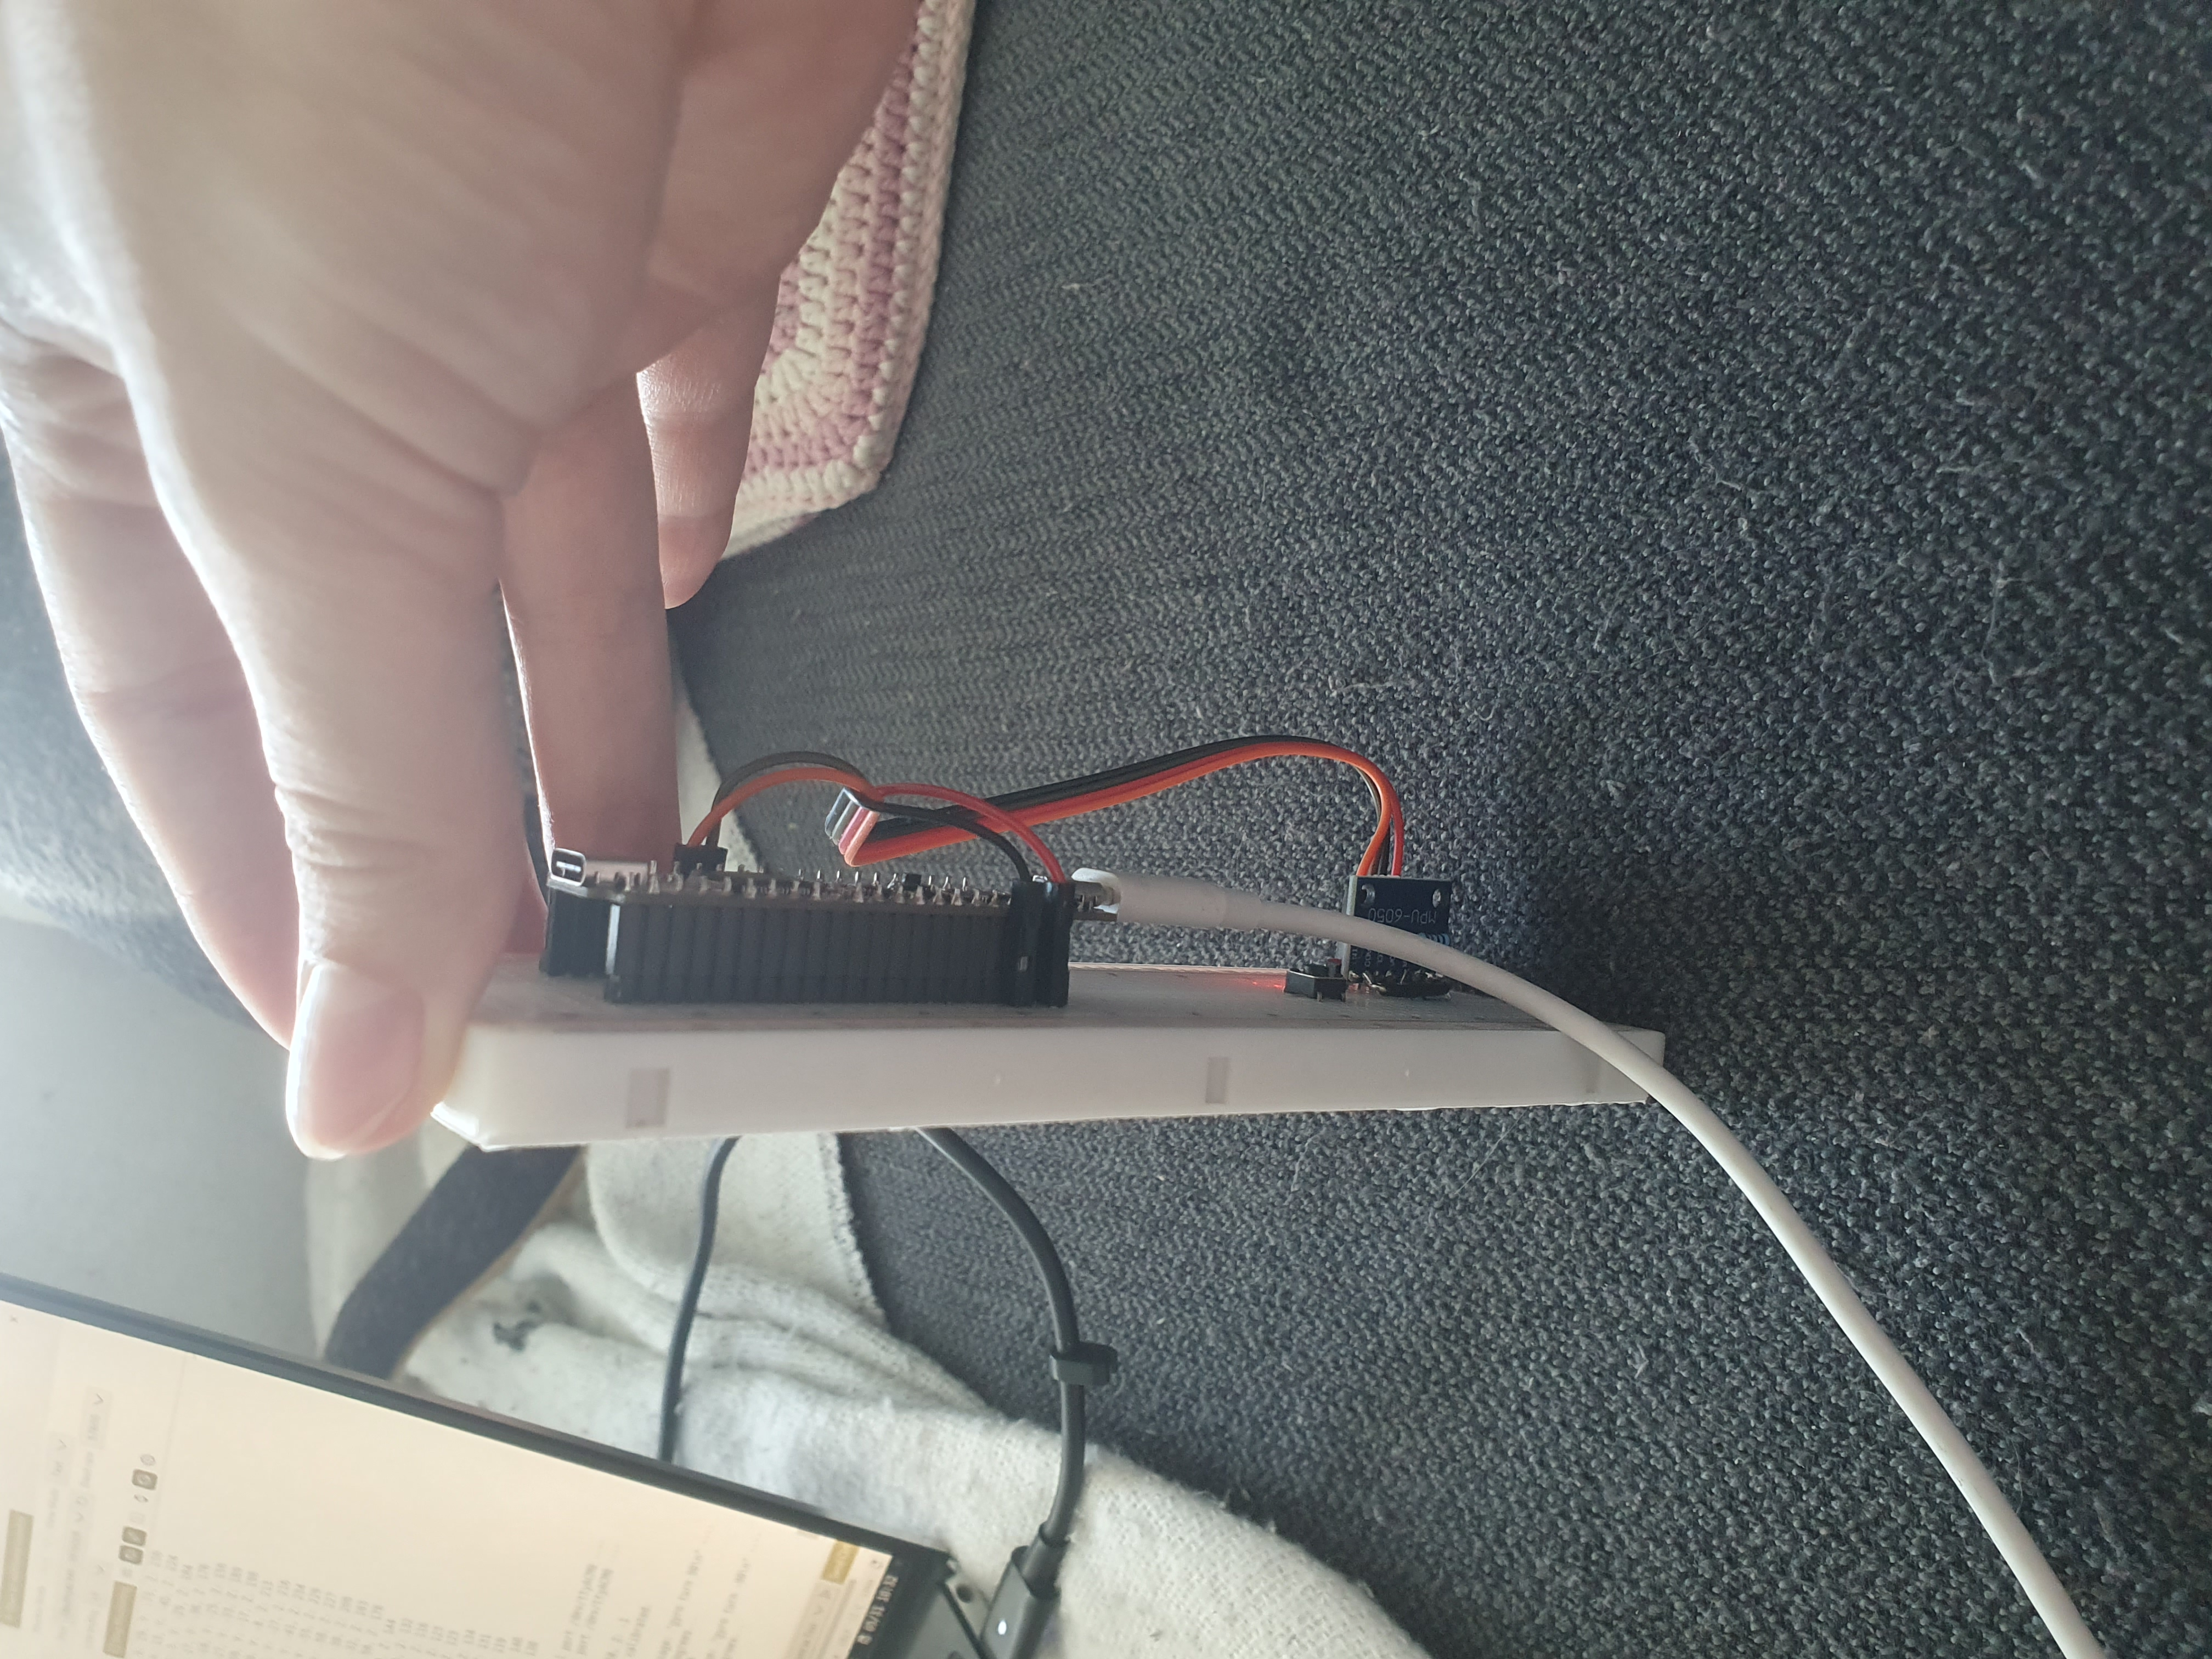
\includegraphics[width=\textwidth, angle=-90]{assets/ET/Gyroskop/gyro-90-deg2.jpg}
    \caption{-90 Grad}
    \label{fig:gyro-90}
  \end{minipage}
\end{figure}

Dazu gab es folgende Ausgabe des Testprogrammes:

\begin{figure}[H]
\centering
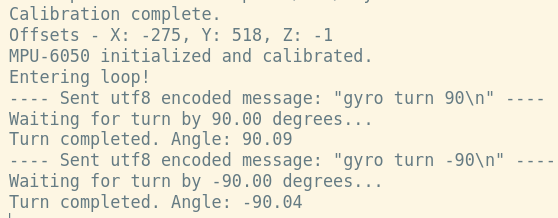
\includegraphics[width=10cm]{assets/ET/Gyroskop/GyroTest.png}
\caption{Ausgabe 90 Grad Drehung}
\label{img:gyro-tests-base}
\end{figure}

Da aus Platzgründen das Gyroskop vertikal angebracht werden muss, werden die Werte der Y-Achse ausgelesen um die Drehung des Roboters zu messen.

Nachdem das Gyroskop angebracht wurde, wurden die Tests von zuvor wiederholt, indem der Roboter von Hand gedreht wurde, um sicherzustellen, dass die richtige Achse ausgelesen werden. Erst dann wurde der Motor für die Drehung verwendet. Sobald der definierte Winkel erreicht wurden, stoppt der Roboter. Dies funktionierte ebenfalls. Dabei wurde die Drehung jedoch etwas ungenauer. Der Roboter dreht sich ungefähr 10\textdegree \ zu weit, da die Motoren zu langsam ausgeschaltet werden. Dies wird jedoch akzeptiert, da es sich nur um eine kleine Ungenauigkeit handelt, die vom Liniensensor beim Losfahren wieder korrigiert wird.


%%%%%%%%%%%%%%%%%%%%%% nachkorrektur wert hindernis %%%%%%%%%%%%%%%%%%%%%%%%%
\newpage
\subsection*{Hindernis umplatzieren - Nachkorrekturwert}\label{hindernis-nachkorrektur}
  \addcontentsline{toc}
    {subsection}
    {Hindernis umplatzieren - Nachkorrekturwert}

Damit der Nachkorrekturwert, der gefahren werden muss, damit das Hindernis am selben Ort abgestellt werden kann, ermittelt werden kann, werden 10 Testdurchläufe durchgeführt. Dabei wird wiederholt der Roboter das Hindernis aufheben, sich 180\textdegree \ drehen und dann dort wo er ist, das Hindernis wieder hinstellten. Dies jeweiligen Abstellorte wurden mit Postit Zetteln markiert (siehe Abbildung \ref{fig:abstellorte}). Die Mitte von jedem Postit korrespondiert mit der Mitte der Barriere. Auch der ursprüngliche Ort der Barriere wird markiert (siehe Abbildung \ref{fig:roboter-grefit-martkier}). Die Distanzen zwischen dem Abstellort und dem ursprüngliche Ort der Barriere wird gemessen. 

Ein blaues Postit, das den Abstellort markiert, ist 12mm breit. Die Distanz von dem Rand des blauen Postit, das sich am weitesten weg von der Barriere befindet, zu der Mitte der Barriere beträgt 153 mm.

\begin{figure}[H]
  \centering
  \begin{minipage}[b]{0.49\textwidth}
    \centering
    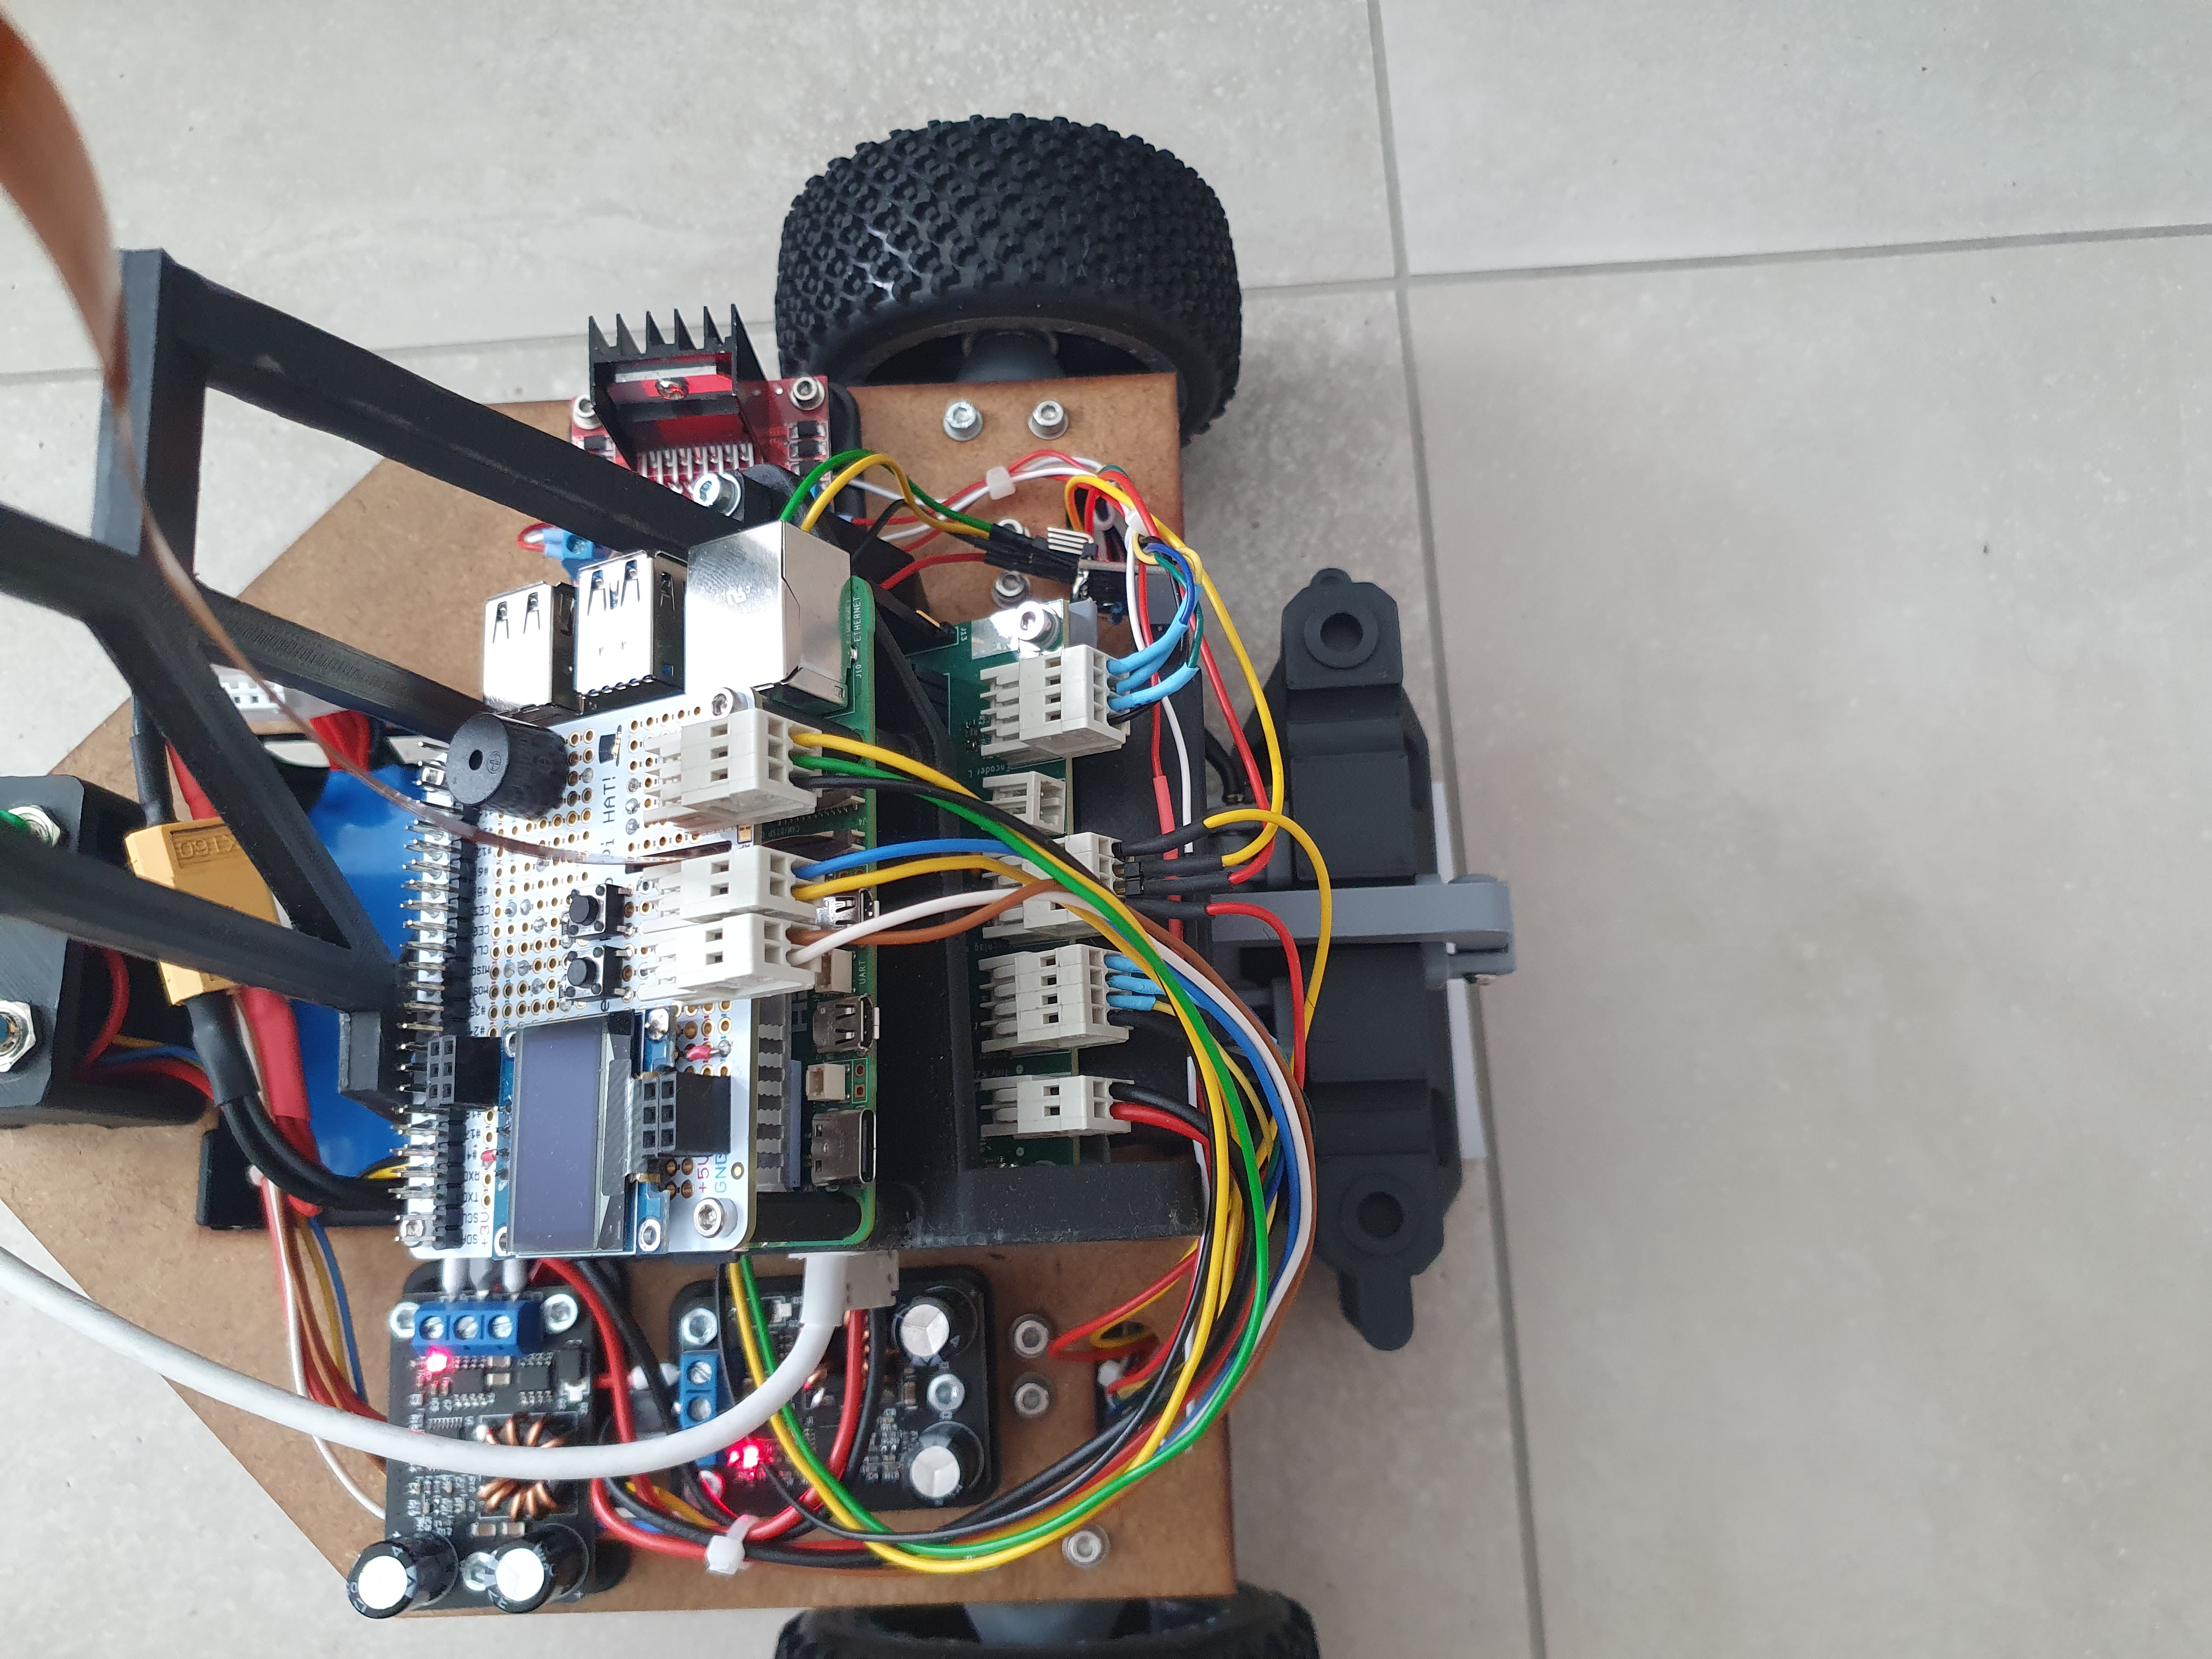
\includegraphics[width=\textwidth]{assets/ET/ultraschall/greifen.jpg}
    \caption{Roboter greift Barriere von markierten Ort}
    \label{fig:roboter-grefit-martkier}
  \end{minipage}
    \hfill
  \begin{minipage}[b]{0.49\textwidth}
    \centering
    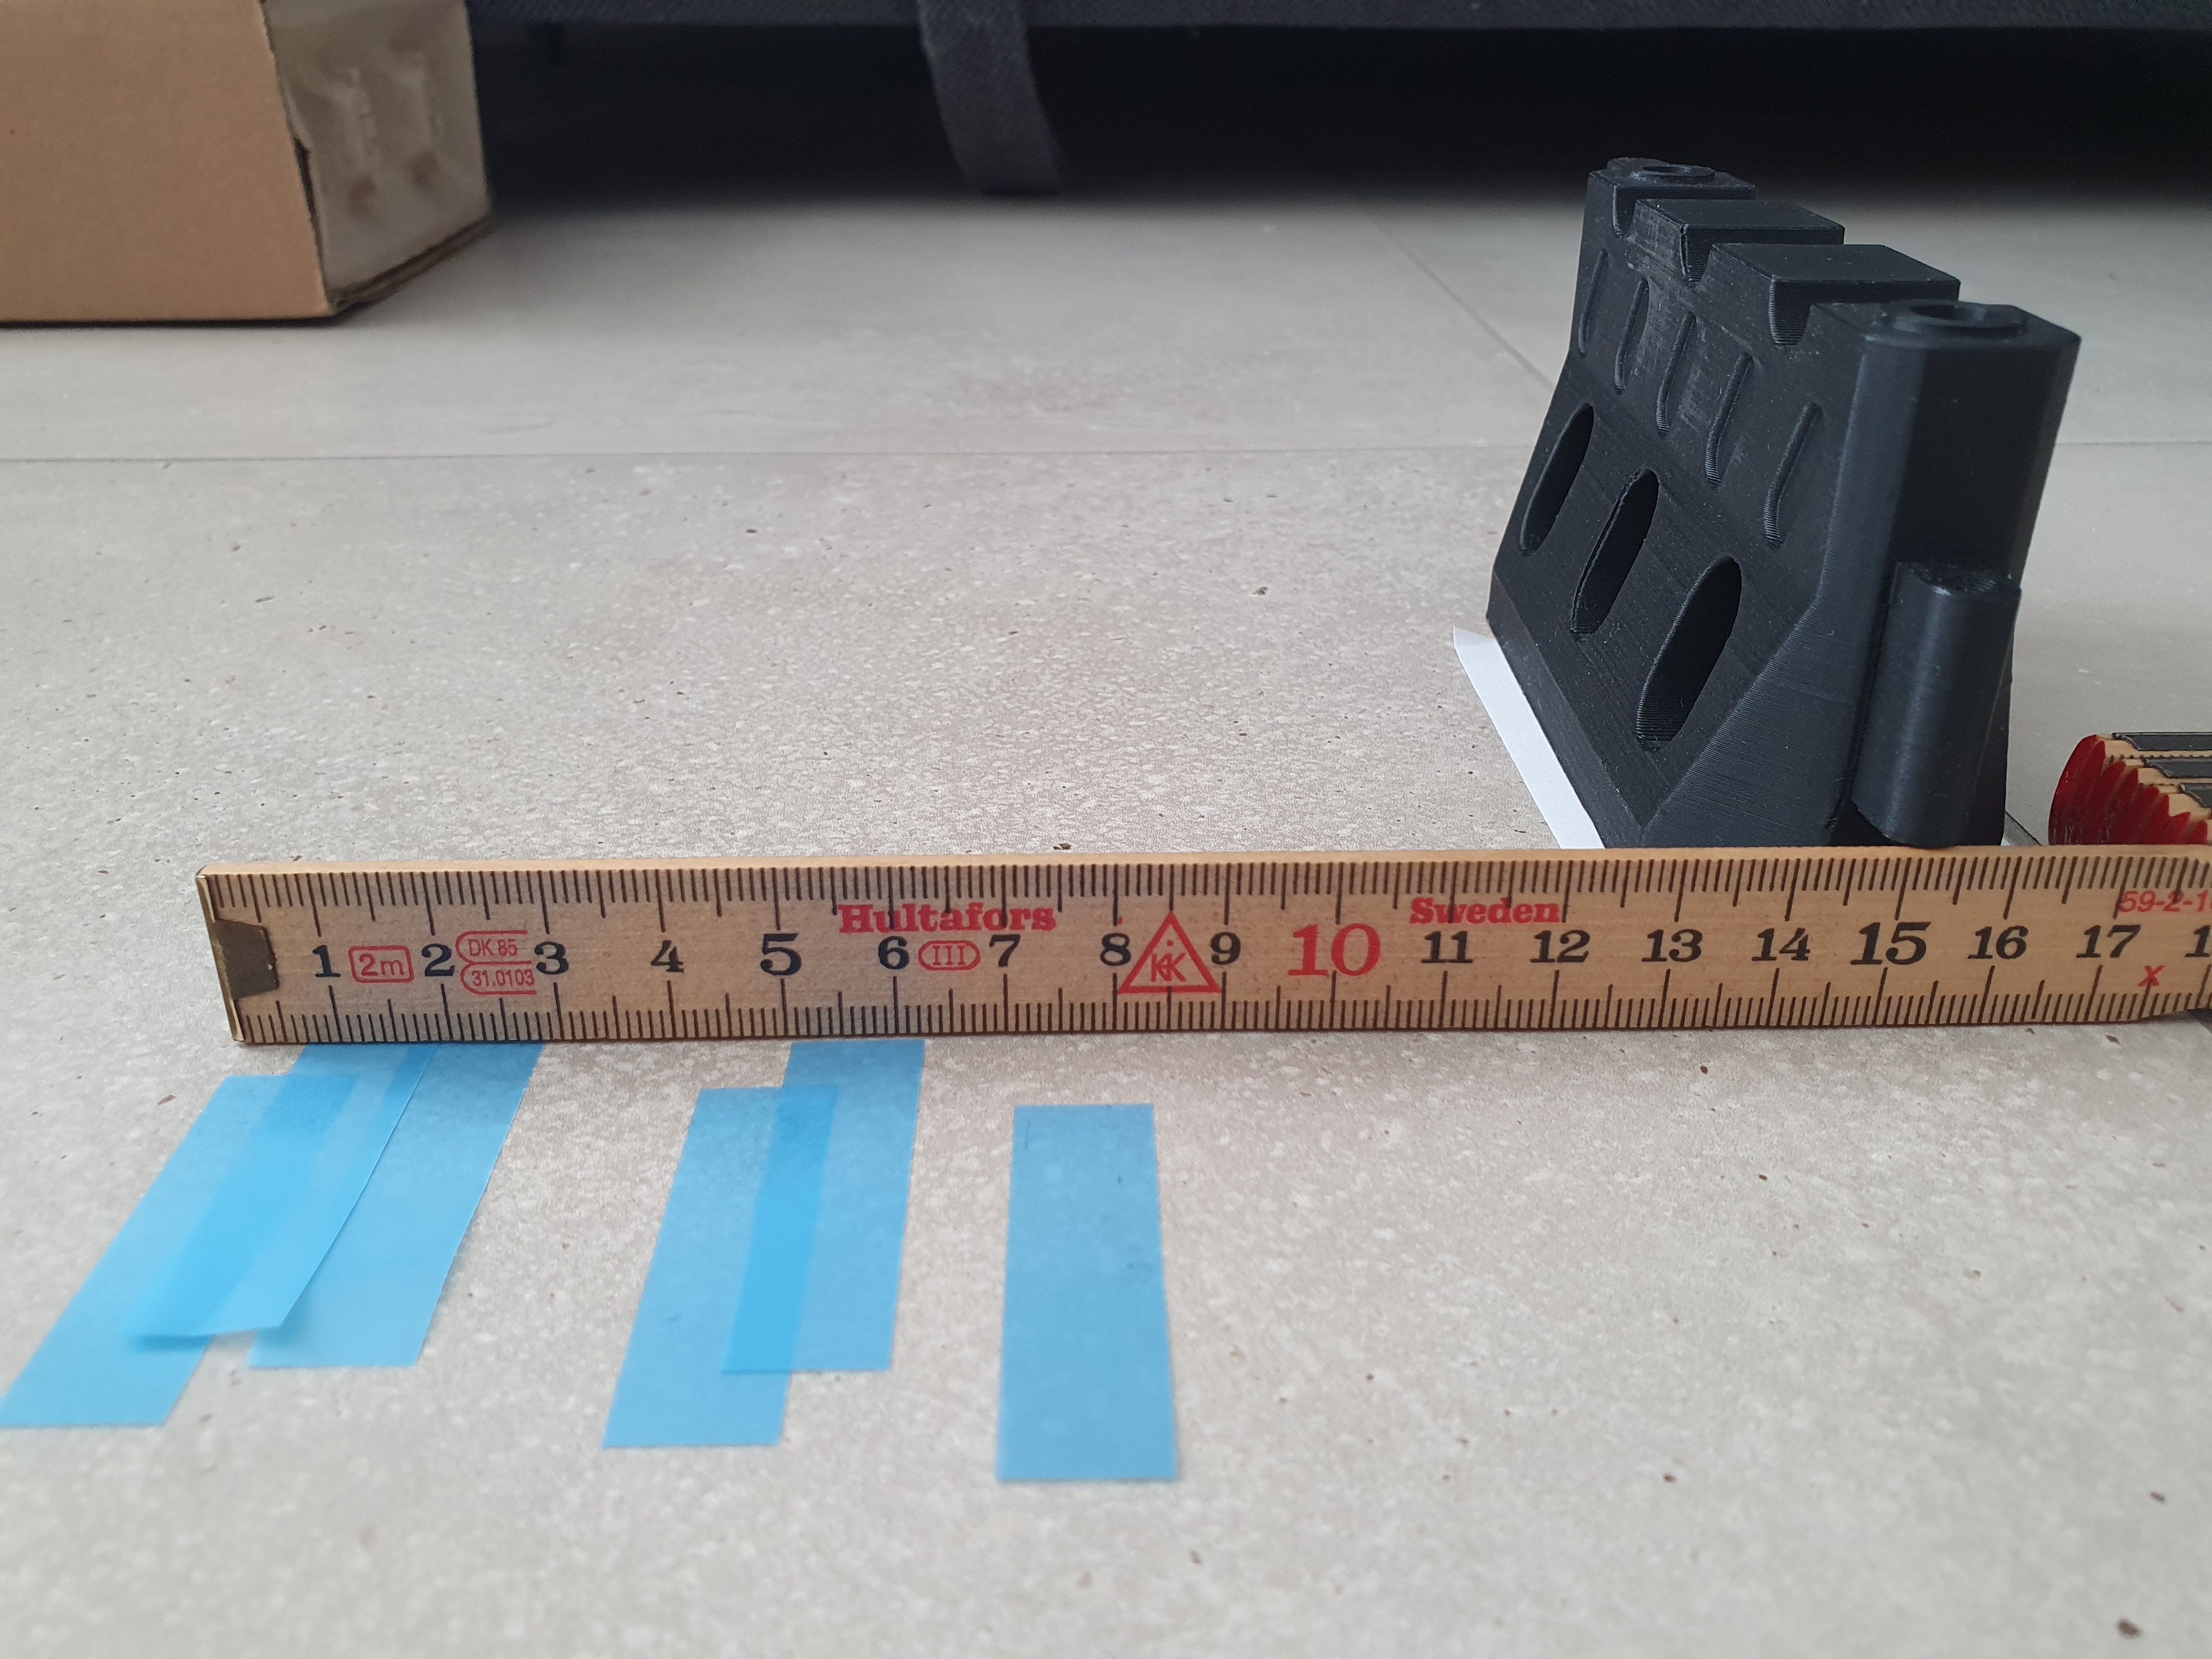
\includegraphics[width=\textwidth]{assets/ET/ultraschall/nachkorrektur.jpg}
    \caption{Alle Abstellorte bei den Testversuchen in blau}
    \label{fig:abstellorte}
  \end{minipage}
\end{figure}

Die Werte aus, die auf dem Bild abgelesen werden können sind hier aufgelistet.

\begin{itemize}
    \item 153mm - 6mm = 147mm
    \item 153mm - 13mm = 140mm (2x)
    \item 153mm - 22mm = 131mm(3x)
    \item 153mm - 50mm = 103mm (2x)
    \item 153mm - 56mm = 97mm 
    \item 153mm - 76mm = 77mm
\end{itemize}

Der Durchschnitt dieser Werte beträgt 120mm. Der Nachkorrekturwert wird auf 120mm gesetzt.


